
This review is based on your 'First version of the Note'. Please put a date on 
successive versions (on the web page as well as on the Note cover page). You 
will find hereafter the comments from the three reviewers (after a round of 
discussions among us). There are some overlapping comments. We left them as 
such on purpose to reinforce the idea, but you may refer to an earlier answer 
in your answer to another reviewer.\\

There are many points to be addressed, but most of them should not take too 
much time. In short, what seems of particular importance to us is:\\
- A better explanation of the RTPC drift speed calibration and track 
reconstruction, and this may entail some rewriting.\\
- Explain from the start what the RTPC gain calibration is or is not used for 
and remove the first method which is not used in the end (or just allude to 
it).\\
- In several instances raised by the three reviewers, check results with 
tighter cuts. It does not necessarily mean that the end results should use 
tighter cuts (e.g. in z-vertex), but that this is a way to study systematic 
effects.\\
- The validity of some 'early' pid cuts (Cerenkov, z-vertex, ...) should be 
checked after exclusivity cuts (for both coherent and incoherent).\\
- The question of accidentals (especially in e-4He coincidences) needs to be 
addressed.\\
- The question of physical background other than exclusive pi0 should be 
discussed, at least qualitatively.\\
This is not to say that the other points are to be dismissed ....

\section*{\centering{$1^{st}$ reviewer}}

~~~~I first have to say that this is of course an unusually complicated and 
difficult analysis (even by CLAS standards) because of the many idiosyncrasies 
concerning the RTPC. Many students and other members of the EG6 collaboration 
have spent an enormous amount of time trying out all kinds of improvements and 
analysis methods, so it would seem like double jeopardy to also insist on an 
equally voluminous tome to describe the analysis. However, I do feel that the 
present version is missing quite a few details that are important for us to 
fully understand what was done, to assess whether it was done 'well enough' and 
to give our green light to the analysis.\\



1) Eq. 2.1, p.16: The second row is missing the charge, q, in front of Bz. This 
is not trivial, as the next 3 lines contain numerical examples that seem to be 
wrong. For instance, the range in $r_{0}$ quoted for DVCS is 20 - 45 mm - but I 
find a radius of 100 mm for 260 MeV/c 4He nuclei going radially (q = 2e). Even 
at some angle, 20 mm is impossible - such a track would never make it through 
the drift region. (Fig. 2.7 shows a minuscule pedestal below $r_{0}$ = 25 mm, but 
this must be due to some spurious effect - I don't see how you can reconstruct 
any tracks with $r_{0}$ < 30 mm). Is this mistake in your software as well (see 
horizontal scale in Fig. 2.7)?\\
\textcolor{blue}{
   In equation 2.1, the charge of the particle (q) is indeed missing. Regarding the 
numerical calculations of $r_0$ for the elastic and the DVCS $^4$He, the 0.3 
factor is missing only in these calculations while the charge issue is taken 
into account. In the reconstruction software, both issues are properly 
implemented. (For example, In a magnetic field of 4.5 T, the recoil 4He nuclei 
from DVCS (elastic) reaction have kinetic energies in the range [10, 25] ([17, 
35]) MeV, from momenta of [260, 450] ([360, 550]) MeV and $r_0$ [70, 150] 
([130,180]) mm.) }\\

2) Section 2.2: The RTPC calibration procedure is described in 2 steps: Event 
selection (2.2.1) and actual calibration (2.2.2 - 2.2.4) plus noise rejection 
(2.2.5). However, the event selection contains cuts on $r_0$, chi2, z etc.  
which in turn presuppose some initial calibration already. In other words, the 
process MUST be iterative - but I couldn't find a clear summary how this 
iteration was executed (i.e., what was used for the first iteration, how many 
iterations total, etc.). There is a short mention at the bottom of p. 27, but 
no details.\\
\textcolor{blue}{The drift paths and drift speed were first extracted using the 
MAGBOLTZ Monte Carlo simulation. One can find the detailed procedure of 
a similar extraction in the BoNuS analysis note 
(https://www.jlab.org/Hall-B/secure/bonus/publication/BonusAnal110117.pdf).  
Then, we proceeded to derive empirical improvements with many iterations after 
each change that would affect the drift paths, such as the beam-offset
 and gain calibrations of the RTPC. Moreover after each pass, the number of
elastic events used for calibration increased. Overall, this was a long 
process that evolved and improved over the years and we concentrated in the 
note on the description of the final iteration.}\\

3) 2.2.1.1 It would be helpful to have some more background information: What 
is the longest drift time (from the inner radius) for a good track? What kind 
of momentum gives you only 4 hits, and are those events important? (see further 
down, under Fig. 3.19) What is the timing offset between the trigger and the 
shortest drift time (outer radius RTPC)? What is the average drift velocity and 
Lorentz angle? Conversion TDC-> time is given p. 15, but it would be much more 
helpful to have all these basic parameters collected in a single place: 2.1.1 - 
2.1.3 are all good places to summarize these parameters.\\
\textcolor{blue}{
  The longest drift time depend on $z$ but is typically around 6.6 $\mu$s. 
  Four is the number of the active pads for a track, not the number of hits.  
  This value has been found to be reasonable from simulation, it mainly help 
  clean the sample and plays very little role after other cuts. The time offset 
  is 15 TDCs (1 TDC= 114 ns), the average drift velocity is 6.14 $\mu$m/ns and 
  we did not extract the Lorentz angle, but MAGBOLTZ indicated about 20 
  degrees.}\\

4) 3rd bullet: There should also be an upper limit on $r_0$, since it is 
actually $r_0$ = +infinity that is indistinguishable from $r_0$ = -infinity 
(i.e., charge will be unknown). For the same reason, it would be nice to have a 
plot of $1/r_0$ instead of or in addition to Fig. 2.7 \\
\textcolor{blue}{Figure \ref{fig:1overr0} shows the 1/$r_0$
   distribution for a sample of the 1.2 GeV data for all the reconstructed 
   tracks without any requirement. Figure \ref{fig:good_r0} presents the same 
   distribution after requiring reading from at least 4 pads, $sdist$ and 
   $edist$ cuts. We see in figure \ref{fig:good_r0} that selecting 
   $r_0>0$ is already cutting the tail of the distribution. Applying a cut for 
   large $r_0$ would correspond to applying a cut at a larger $1/r_0$. Based on this
   distribution, we do not see any motivation for this. In particular since exclusivity
   cut will eventually clean all unphysical results.}\\


\begin{figure}[tbp]
\hspace{-1cm}
\begin{minipage}[c]{.46\linewidth}
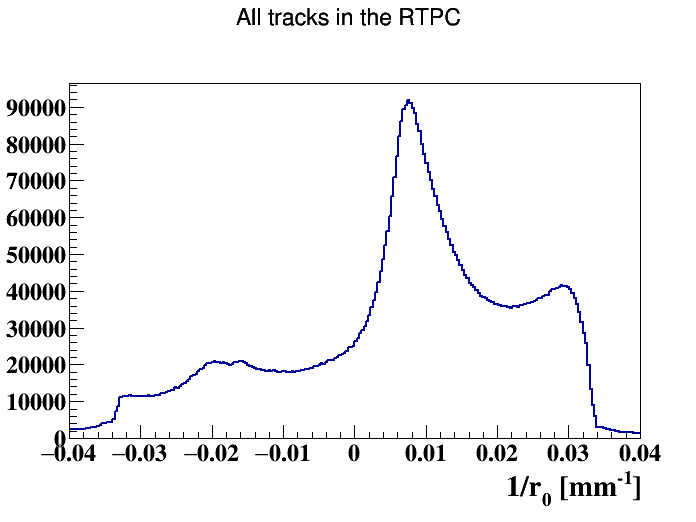
\includegraphics[height=6.5cm]{fig/rtpc_1overr0_all_before.png}
\caption{1/$r_{0}$ for all the reconstructed tracks in the RTPC using 1.2 GeV 
electron beam.}
\label{fig:1overr0}
\end{minipage} \hfill
\begin{minipage}[c]{.46\linewidth}
\hspace{-0.1in}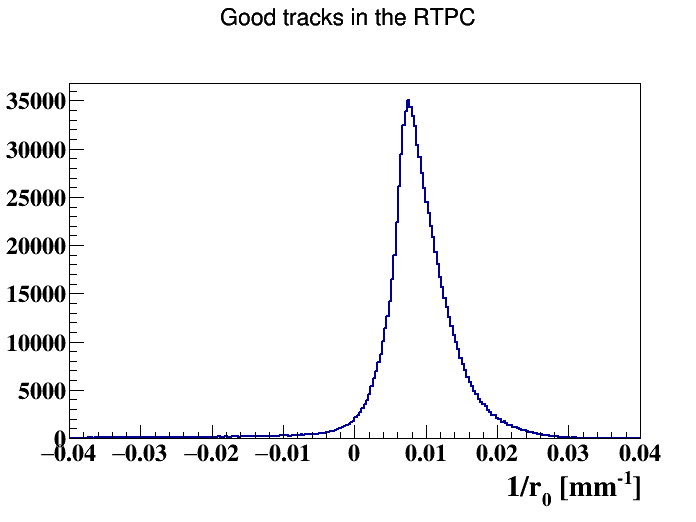
\includegraphics[height=6.5cm]{fig/rtpc_1overr0_all.png}
\caption{1/$r_{0}$ for tracks that passed the requirements: reading from at 
least 4 pads, $sdist$ and $edist$.}
\label{fig:good_r0}
\end{minipage}
\end{figure}


5) 4th bullet: How are the points $r^{helix}$, $\phi^{helix}$ and $z^{helix}$ 
determined?  Somehow, you have to identify points on a continuous line that are 
closest to (perhaps) the hits? How are the uncertainties (sigmas) in  
$\chi^{2}$ determined?  Are those the final values AFTER calibration? If so, 
how do you select your sample initially? (See above - it must be an iterative 
process).  \\
\textcolor{blue}{$(r^{helix},\phi^{helix},z^{helix})$ is the point
on the helix that is closest to the reconstructed hit position.
The values of the uncertainties are intrinsic detector properties depending
primarily on the size and configuration of the readout pads. These 
uncertainties, $(\sigma_{r}, \sigma_{\phi}, \sigma_{z}) = (0.53 mm, 2^{\circ}, 
1.2 mm)$, were not derived from our data and were held fixed over all 
calibration itterations.} \\
\textcolor{blue}{Equation 2.2 needs the beam-spot constraint added in
quadrature $\left(\frac{DOCA}{\sigma_r}\right)^2$ as follows (changed in 
the note as well): }\\

\textcolor{blue}{
\begin{equation}
   \chi^{2} = \frac{\displaystyle \left(\frac{DOCA}{\sigma_r}\right)^2 
       + \sum_{i = 1}^{ N_{pts}} \left(\frac{r^{pt}_{i} 
      - r^{helix}_{i} }{\sigma_{r}}\right)^{2}  + \left( \frac{\phi^{pt}_{i} - 
      \phi^{helix}_{i} }{\sigma_{\phi}}\right)^{2} + \left( \frac{z^{pt}_{i} - 
   z^{helix}_{i} }{\sigma_{z} } \right)^{2}}{N_{pts} - 4}
\end{equation}
}\\



6) 5th bullet: Again, $sdist$ and $edist$ already pre-suppose a timing 
calibration.  For assessing possible accidental coincidences (see more below), 
it would be useful to know what time spans correspond to the limits chosen on 
them.\\
\textcolor{blue}{ $sdist$ limits span a drift time equal to 0.68 $\mu s$, while 
$edist$ limits span 1.03 $\mu s$.}\\

7) Finally, I'm puzzled by the large positive limit on $edist$ - supposedly this 
quantity is easier to measure (shortest 'drift' time), yet there is clearly a 
tail towards positive $edist$ (towards smaller radii??) superimposed on an 
otherwise sharp peak. Wouldn't you want to cut that tail at least for the 
purpose of calibration, to make sure you only look at 'golden tracks'? Is it 
specific to higher momenta? \\
 \textcolor{blue}{
The positive long tail on $edist$ distribution is made of hits out of time 
mostly due to electronic noise. However, if we do not apply any constraint on 
$edist$ and $sdist$ variables and select the elastic He-4 tracks with the other 
cuts, we observe that most of the tails are removed as can be seen in the 
figure~\ref{fig:sdist} and \ref{fig:edist}. Therefore, making tighter cuts 
would not cause changes in the calibration as the tracks in the tail regions 
are cleaned by the other cuts.  No correlations was observed between the tails 
and the momentum, as can be seen in figure~\ref{fig:edistp}.}\\

\begin{figure}[!h]
\begin{minipage}[c]{.46\linewidth}
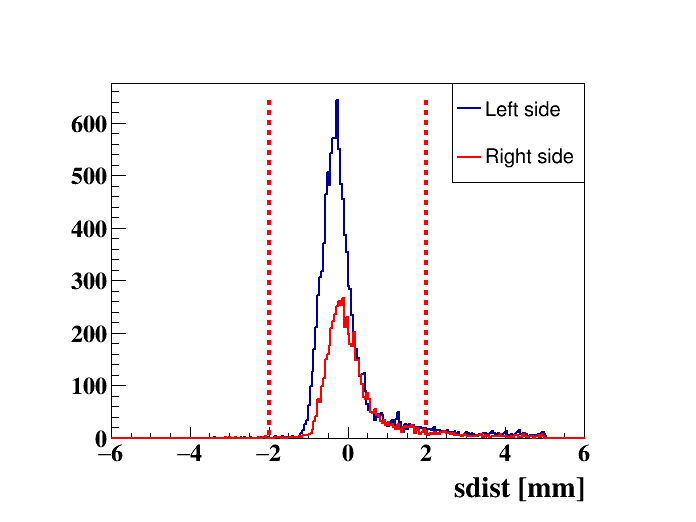
\includegraphics[height=6.5cm]{fig/sdist_elastic_1p2GeV.png}
\caption{sdist distribution for the selected elastic $^{4}$He tracks.}
\label{fig:sdist}
\end{minipage} \hfill
\begin{minipage}[c]{.46\linewidth}
\hspace{-0.1in}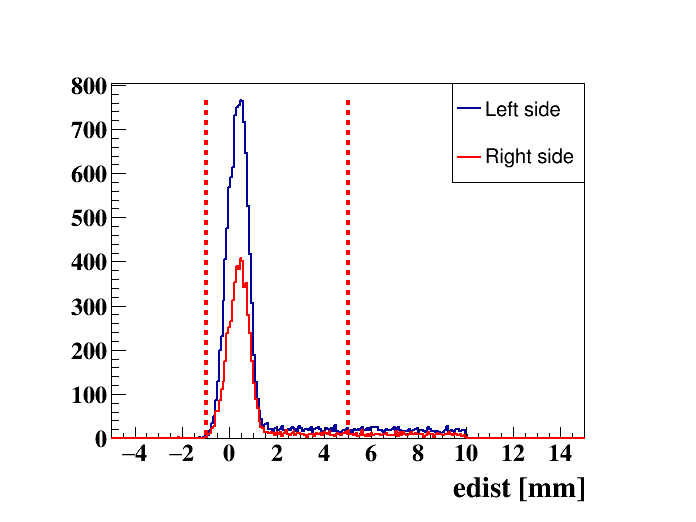
\includegraphics[height=6.5cm]{fig/edist_elastic_1p2GeV.png}
\caption{edist distribution for the selected elastic $^{4}$He tracks.}
\label{fig:edist}
\end{minipage}
\end{figure}

\begin{figure}[!h]
\centering
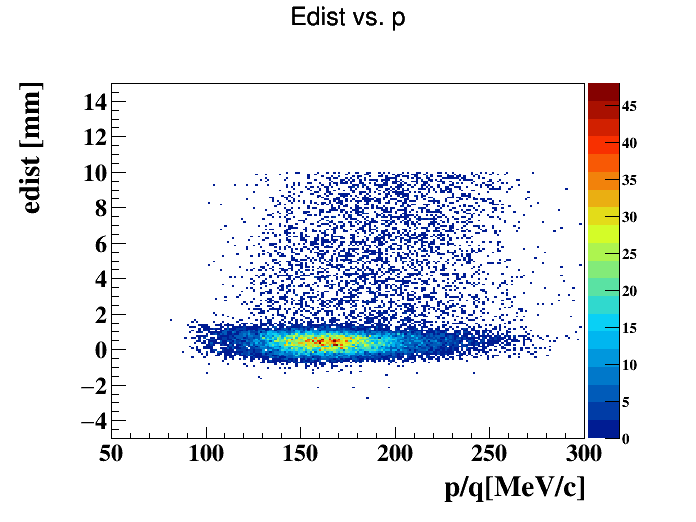
\includegraphics[height=6.2cm]{fig/edist_poverq_elastic_1p2GeV.png}
\caption{edist as a function of the measured p/q for the selected elastic 
tracks.}
\label{fig:edistp}
\end{figure}


8) Last bullet: Again, what are the initial choices on this cut to select 
calibration tracks? What do you use for the $z_0$ of the simulated track?  \\
\textcolor{blue}{
   We used similar cuts for all the calibration iterations. $z_0$ of the 
simulated $^{4}$He is set to be the z-vertex of the scattered electron. The 
2$\sigma$ cut corresponding to $\approx$ 20 mm.  }\\

9) 2.2.1.2 Again, these cuts already pre-suppose (good enough) initial tracks.  \\
\textcolor{blue}{Yes}\\

 10) Fig. 2.11: Do we understand why $\Delta z$ is not constant? Is this before 
or after the RTPC alignment (alluded to but not explained)? Is the resolution 
shown the final result after optimizing the calibration? The exact same 
questions also arise for Fig. 2.12. \\
\textcolor{blue}{
  The presented $\Delta z$ and $\Delta\phi$ distributions are after all the 
calibration and detector alignments (RTPC alignment is described in CLAS-NOTE-2013-008).
The observed remaining dependences are not fully understood and probably arise
from field misalignement and variations in the electric and magnetic fields
within the chamber.} \\


11) Eq. 2.4: It is much better to use a cut on the reconstructed beam energy 
from the measured angles $\theta_e$ and $\theta_{He}$, since momenta are less 
precisely measured by CLAS than angles. Peter Bosted has used this method very 
effectively. Indeed, Fig. 2.13 shows a rather broad distribution, with a cut 
that barely has any effect. (This is a side comment, not meant to require 
additional work).\\
\textcolor{blue}{We are indeed aware of this and we do use a $\Delta \theta$ cut
as our main selection for this reason, which we believe is equivalent to your
proposition. Note also that $\Delta\phi$ and 
$\Delta z$ cuts have already been applied in Figure 2.13's $\Delta\theta$.}\\

12) Fig. 2.14: It's curious that the W distribution 'for the right RTPC module' 
is wider than on the lhs, given that nothing measured by the RTPC enters this 
quantity. However, it might be that the corresponding sectors in CLAS have 
different resolution, as well.\\
\textcolor{blue}{
Yes, this is related to the different resolutions of the corresponding CLAS sectors. 
This effect is large because, the reaction products are emitted back to back 
resulting in small regions of overlapping acceptances of the RTPC and CLAS.  
In figure \ref{fig:W_sec}, we plot $W$ distributions corresponding to the 
different sectors in CLAS, one can immediately see the differences of resolution.}\\

\begin{figure}[!h]
   \centering
   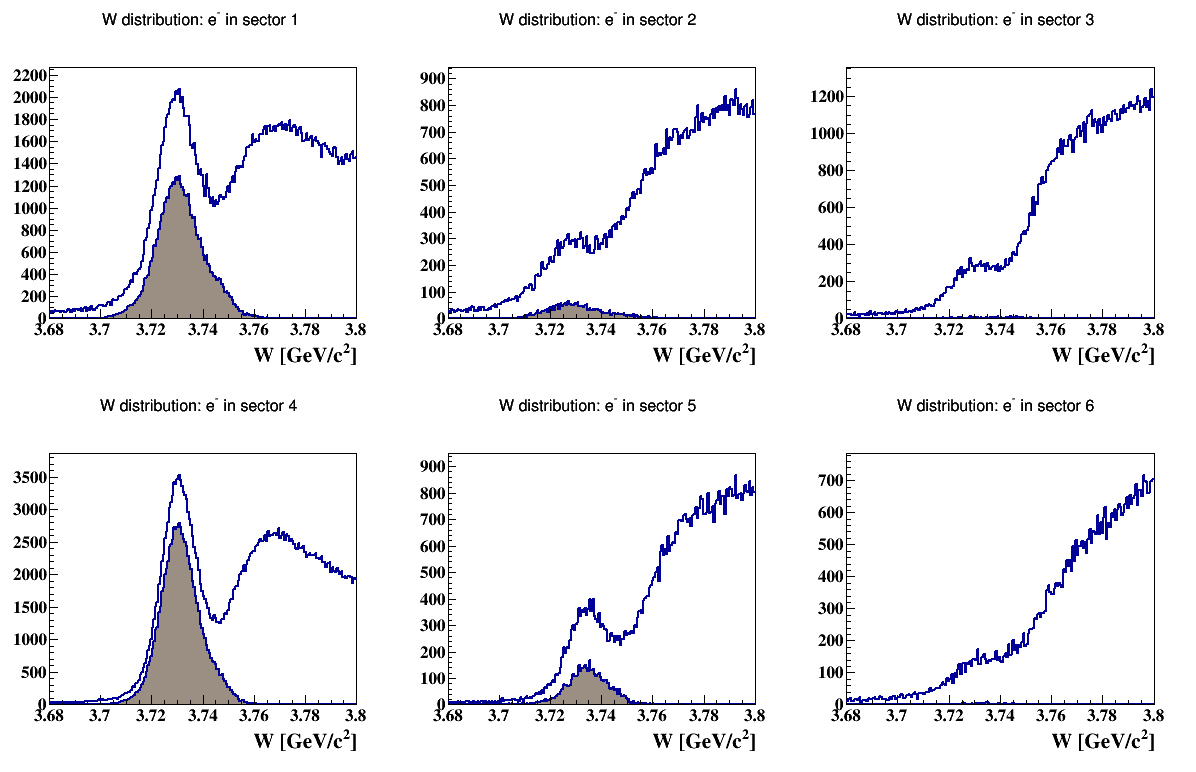
\includegraphics[height=10.5cm]{fig/W_dis_sectors.png}
   \caption{W distributions for the identified good tracks (in blue) and 
   elastic events (in shaded brown) where the electron scattered in the 
different sectors of CLAS.}
   \label{fig:W_sec}
\end{figure}


- 2.2.2 2nd paragraph: Due to the varying B(z) and therefore the varying 
Lorentz angle, the drift path is NOT the same for all electrons at all z.  
(Corrected in the 3rd paragraph.)
More importantly, all times are given in TDC units instead of $\mu$s- we must 
know the conversion factor and the offset! (Is it the same for all TDC 
channels?)\\
\textcolor{blue}{1 TDC = 114 ns, the time offset is TDCmin (= 15 TDCs) and is 
the same for all the readout channels.}\\

13) Fig. 2.19: I can't figure out what exactly is plotted here (in particular 
on the z-axis). If I understand Eq. 2.8 correctly, then R is simply deduce from 
TDC for the real data - so no surprise to see a straight line. How is this then 
linked to the simulated track?\\
\textcolor{blue}{Here R is from simulation and TDC is from real data. This 
figure is indeed here only to illustrate the Eq 2.8 and allows to associate
simulated hits with measured ones. The text is modified to clarify this 
point.}\\


14) Figs. 2.20-22: Again, more detail needed to understand what's plotted and 
how it is calculated. Why is Delta-phi not zero for TDC = 15 (which corresponds 
to the outer radius of the drift region)?- Eq. 2.9: A (brief) derivation would 
help a lot here.\\
\textcolor{blue}{
$\Delta \phi$ at the anode (TDC = 15) is not equal to zero because there is a 
drift in $\phi$ between the anode (the first GEM layer at radial distance equal to 
60 mm) and the readout pads (at radial distance equal to 69mm). Regarding the 
derivation, figure \ref{fig:drift_derive} shows a simple drawing explaining how 
Eq. 2.9 can be derived.}\\

\begin{figure}[!h]
   \centering
   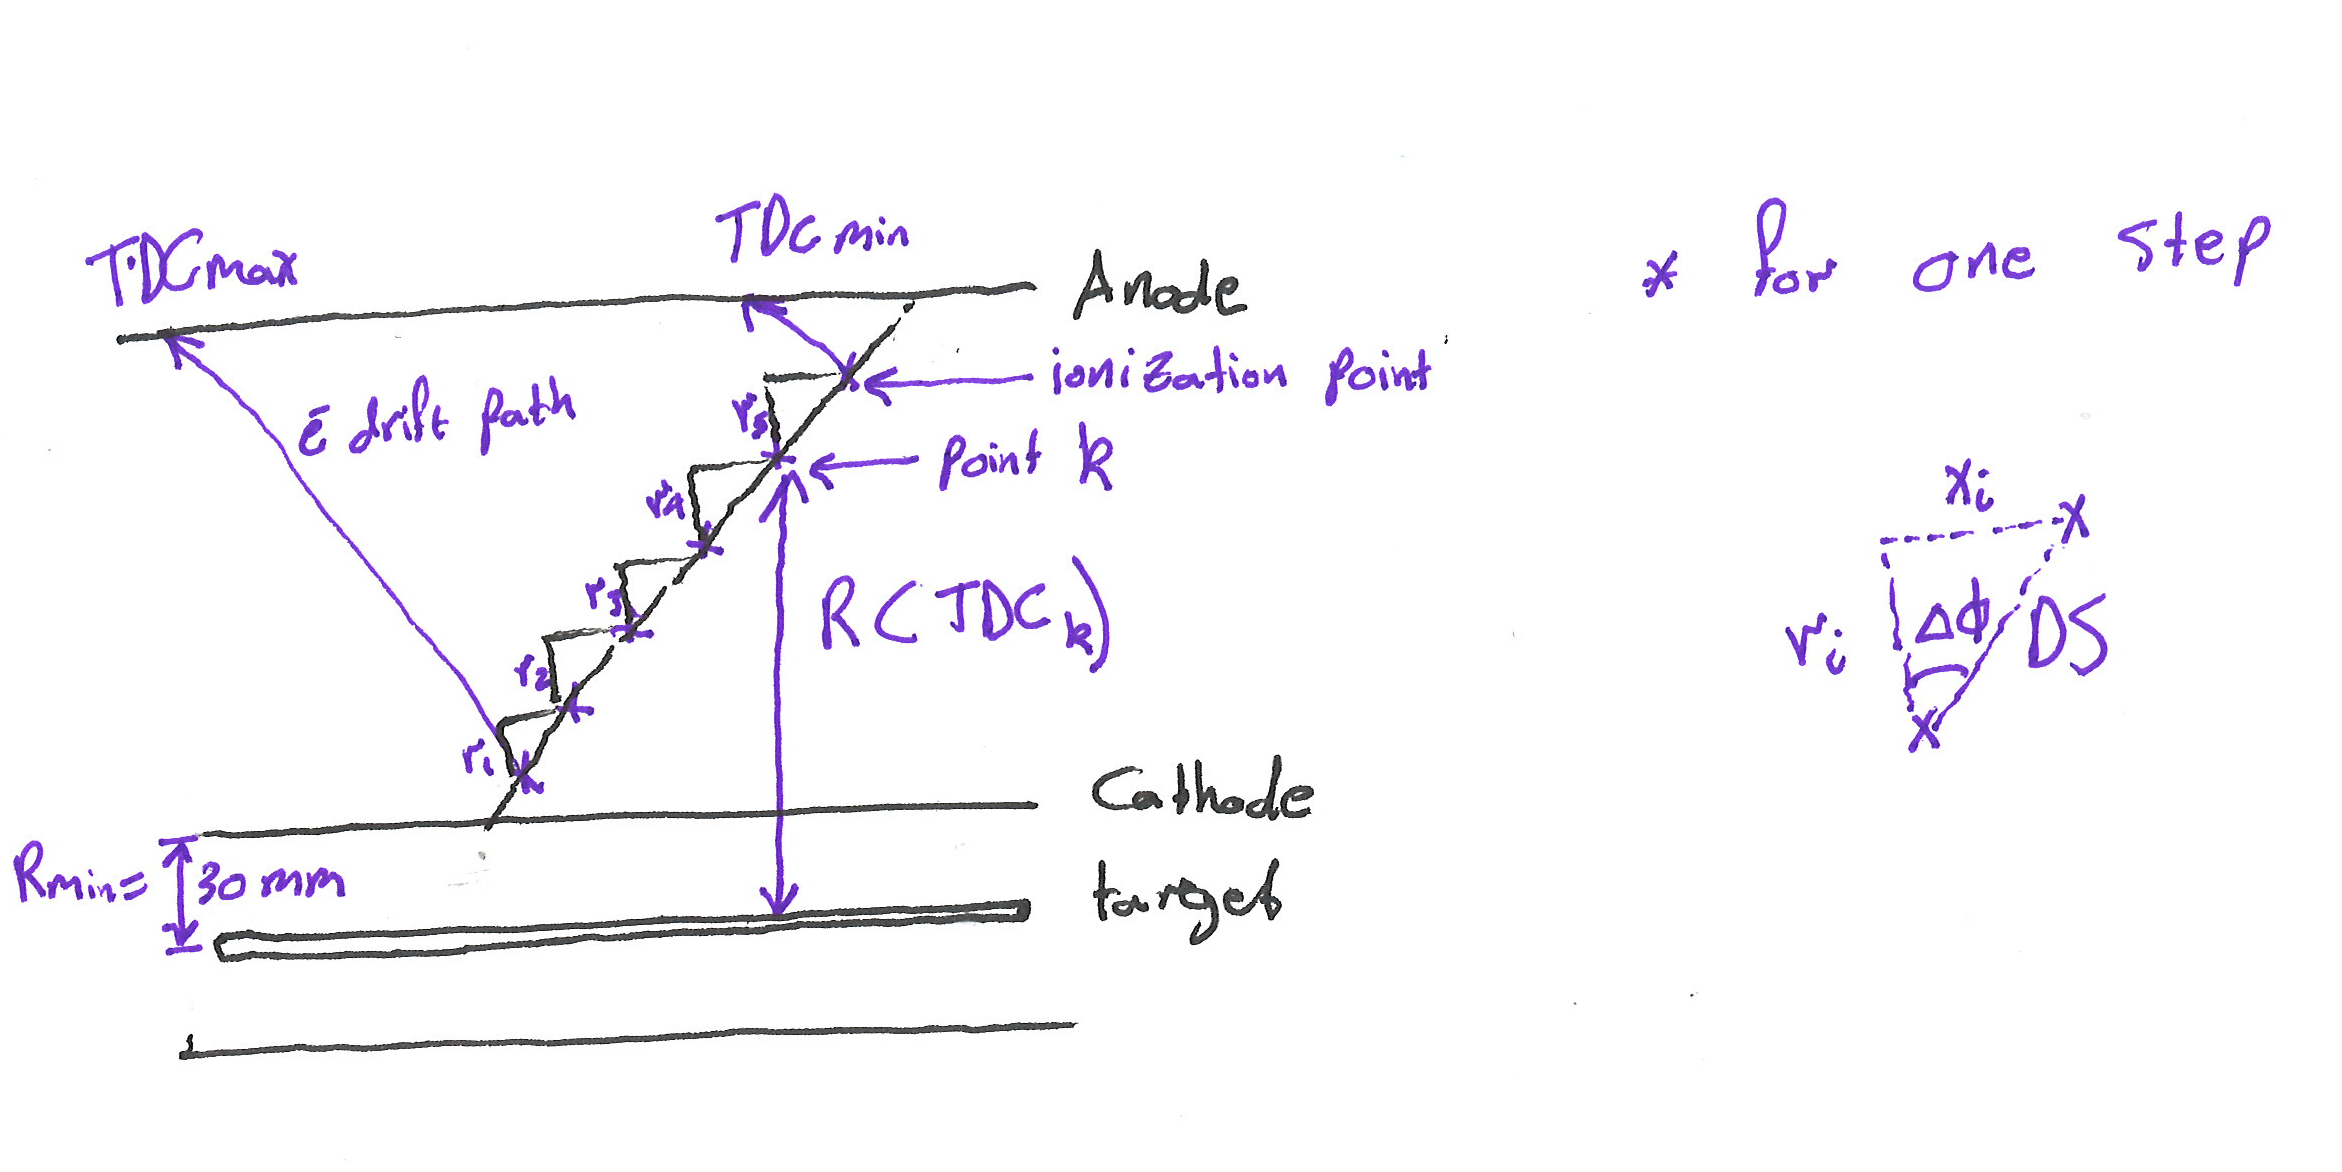
\includegraphics[height=6.5cm]{fig/deriv_R_drift.png}
   \caption{Schematic drawing shows how the radius of emmision (R) at each 
   ionization point is calculated from the drift paths ($\Delta \phi$) and the 
drift speed ($DS$).}
   \label{fig:drift_derive}
\end{figure}
\textcolor{blue}{In figure \ref{fig:drift_derive}, the radial distance of the 
   ionization point $k$, $R(TDC_{k})$, is equal to to the radial distance from 
   the target to the cathode, $R_{Min}$, plus the radial distances ($\sum 
   r_{i}$) that are caused by the drift from the first point of ionization at 
   $TDC_{max}$ to the point $k$. In each TDC bin, the radial drift distance 
($r_{i}$) is calculated as:}

   \begin{equation}
      r_{i} = \sqrt{DS^{2} - r_{i-1}  \bigg(\frac{\partial \Delta \phi} 
      {\partial TDC}(TDC_i) \bigg)^{2} }
\end{equation}
\textcolor{blue}{Adding all the terms, $R(TDC_{k})$ is formulated as:}
\begin{equation}
   R (TDC_{k}) = R_{min} + \sum\limits_{i=TDC_{Max}}^{TDC_{k}} r_{i}
\end{equation}

15) 2.2.4: Eq. 2.12 is differential, while Eq. 2.14 is integrated over the 
whole track. Do you integrate Eq. 2.12? Otherwise, it probably doesn't work all 
that well. Maybe this is the reason why the bands visible in Fig. 2.29 are not 
well represented by the superimposed curves? BTW, what is the vertical scale on 
Fig. 2.29?\\
\textcolor{blue}{Eq. 2.14 represents the average energy loss per unit of length in the 
track, $vtl$ being the visible track length. Assuming the energy loss in the 
drift region small, the two can be easily compared. Indeed at the lowest energy 
this assumption is not true anymore. But the difference between instantaneous 
and average $\frac{dE}{dx}$ is expected to be small compared to our 
resolution except very close to threshold (see right panel of Figure 
\ref{fig:energylosscorrection}).} \\
\textcolor{blue}{In Fig. 2.29 the lines are just there to guide the eye. Since the
vertical scale has never been carefully calibrated, we always present it in
arbitrary units. To have a feeling of the units, we have extracted an over all 
conversions from comparing real data to simulation, where 1 ADC is equal to 17 eV 
(21 eV) deposited in the left (right) module of the RTPC.} \\


16) p. 29, 2nd to last paragraph: I THINK I understand the Landau fit (over 
many tracks, no?) for each channel. But I don't understand the last step - why 
is it needed? What does it accomplish? For sure more details (and a plot) are 
needed.\\
\textcolor{blue}{
Yes, the gain ratio of each readout pad is calculated from comparing all the 
experimental elastic tracks to their corresponding tracks obtained from 
simulation. These ratios give us a first gain for each readout pad. However, 
we noticed that some pads record lower ADCs than expected (issue shown in 
figure 2.28) and sometime noise. For these reasons, we wanted to make sure that the recorded 
ADCs by a given pad are similar to the recorded ADCs recorded by another pad in 
the same track. In figure~\ref{fig:dedxre}, one can see improvements obtained
by using this method to fine tune the gains obtained previously.} \\

\begin{figure}[!h]
\hspace{-0.5 cm}
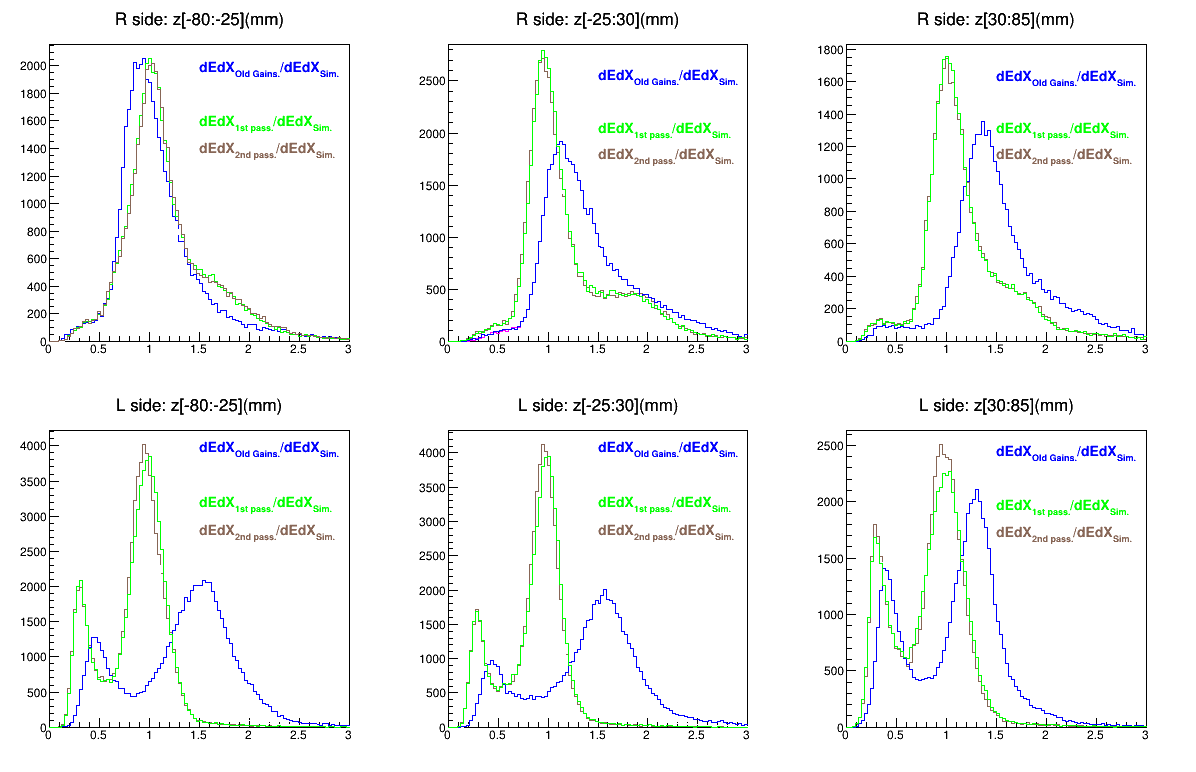
\includegraphics[height=11.5cm]{fig/dedx_ratio_elastic_NAB.png}
\caption{The ratio between the experimental dEdx and the simulated ones for 
   different regions along $z$ of the RTPC. The blue lines are using the first 
   method of extracting the gains (comparing the experimental recorded dEdx to 
   the expected values calculated from the Bethe-Block formula), the green 
lines are using the 1st pass of the second method (comparing simulation to data 
only) with all the elastic event sample and the brown lines are using the gains 
extracted from the second method (both steps).}
\label{fig:dedxre}
\end{figure}

17) p.31, last paragraph: Could it be that the low-signal tracks are due to 
protons (maybe elastically scattered out of the Kapton target enclosure)? There 
could be some beam halo interacting with the straw tube. Last sentence (top 
p.32): HOW are 'events from the low-region' excluded from the analysis (for 
NON-elastic events)? Do you use a cut on dE/dx? Describe the cut! (It's not 
mention in Section 3.1.4 - but why bother with gain calibration if you don't 
use the ADC values?)\\
\textcolor{blue}{More work is needed to understand the nature of these 
low-signal tracks, but they cannot be protons as their dedx would be much smaller,
and they are only present in one half of the RTPC.  We looked hard but found no
correlation between these tracks and any other experimental quantities.
A possible explanation is that the gain might have been periodically
lowered by high rates of events. For this DVCS analysis we do 
not use $\frac{dE}{dx}$ to select $^4$He, instead we only use the DVCS 
exclusivity cuts.
Figure \ref{fig:dedx_good_6gev} shows dEdx as a function of $p/q$ 
for the good tracks from 6 GeV beam energy runs, while Figure 
\ref{fig:dedx_dvcs_6gev} shows the same for identified coherent DVCS He-4 
nuclei. One can see that the selected He4 nuclei have on average high dEdx 
trend that matches with the theoretical line, 
but the band seem too wide to apply a significative cut.} \\


\begin{figure}[tbp]
\hspace{-1.0cm}
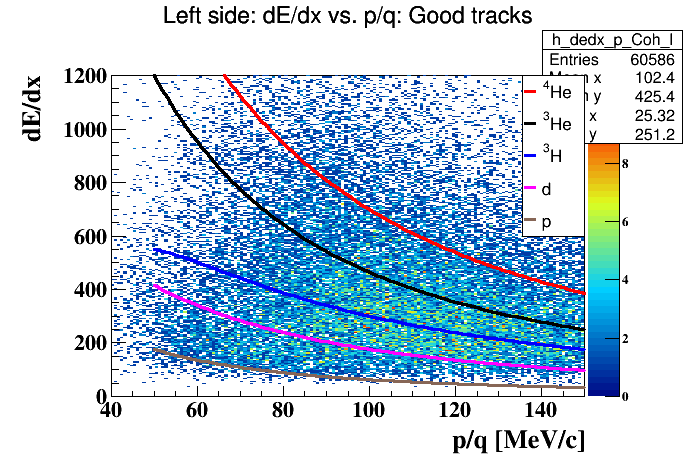
\includegraphics[height=6.2cm]{fig/dedx_p_Coh_l_good.png}
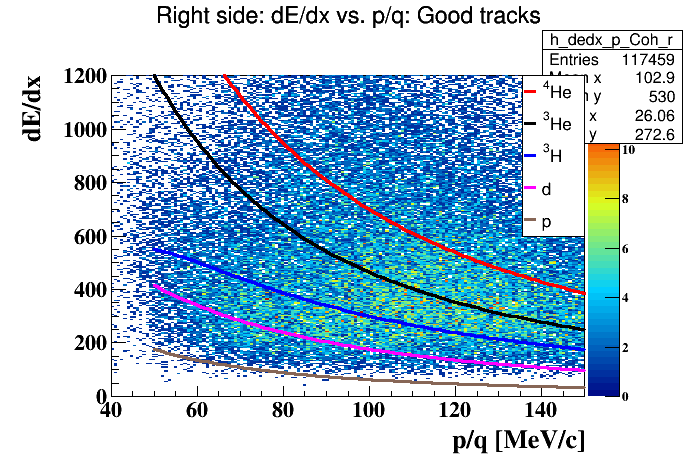
\includegraphics[height=6.2cm]{fig/dedx_p_Coh_r_good.png}
\caption{dEdx verus $p/q$ distribution for the good tracks collected at 6 GeV 
beam energy.}
\label{fig:dedx_good_6gev}
\end{figure}

\begin{figure}[tbp]
\hspace{-0.1cm}
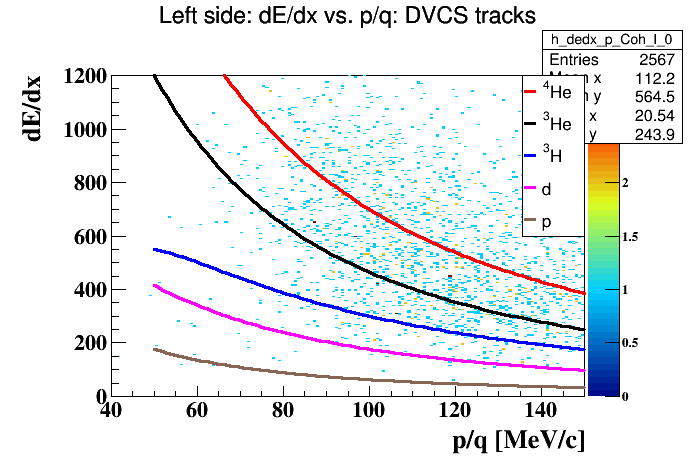
\includegraphics[height=6.2cm]{fig/dedx_p_Coh_l_dvcs.png}
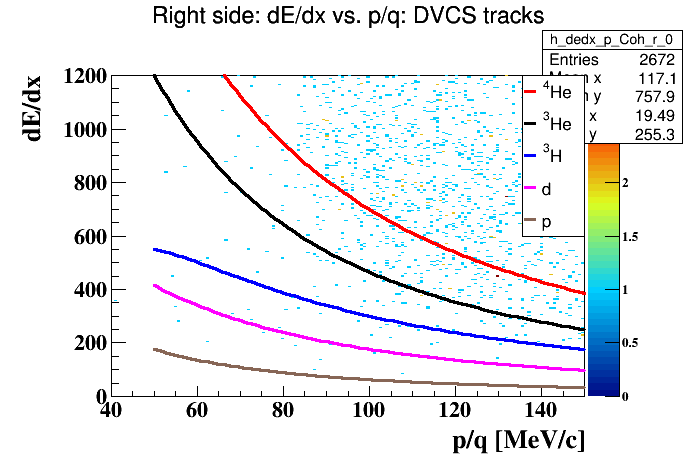
\includegraphics[height=6.2cm]{fig/dedx_p_Coh_r_dvcs.png}
\caption{dEdx verus $p/q$ distribution for the identified He4 DVCS nuclei at 6 
GeV beam energy.}
\label{fig:dedx_dvcs_6gev}
\end{figure}


18) 2.2.5: 3rd line, the claim is made that elastic 4He produce too small a 
signal because of their small Tkin. This is strange, since low Tkin actually 
means LOTS of energy LOSS - which is also born out by Fig. 2.29. Overall, it 
would be good to get a quantitative feeling for the amplitude of the noise (in 
mV and in equivalent dE/dx relative to good 4He tracks). It would be even 
better if we had any inkling about the source of the noise (electronics 
malfunction? cross-talk? antenna pick-up?), but of course that's not a 
requirement for the analysis to be approved. \\
\textcolor{blue}{
The statement about too small Tkin is misleading and has been changed.
The fact is that readout thresholds were set low to avoid efficiency problems,
with the effect of recording more electronic noise. We do not know where the noise is
coming from, only speculation. As for getting a feeling of the
amplitude of the noise, one option is to compare Figures 2.30 with 2.25 and/or
2.28 top. This shows that the amplitude of the oscillatory noise is not much
smaller than the typical hits from a $^4$He track.}\\
    

19) Fig. 2.30: What is plotted on the z-axis? (Occupancy?) Is this plot 
integrated over all 'good tracks', or only for tracks that actually traversed 
the selected pad (or a nearby pad)? If the former, what does a signal for a 
good track that crosses this pad look like?\\
  \textcolor{blue}{The color scale on the $z$-axis is a hit yield. The
hits included are only those recorded by one example noisy pad and only when
those hits were used in a good track.} \\


20) 2.3: 5th line p. 37: No, the z-vertex resolution for an extended target in 
the presence of the DVCS solenoid is a lot worse than 1 mm - see Fig. 3.1 So in 
fact the z-resolution of the RTPC is not that bad.\\
 \textcolor{blue}{Indeed the indicated value is without solenoid. In the presence of 
the solenoid, the z-vertex resolution of 
CLAS is about 3 mm, which we measured from the downstream target 
window, as can be seen from figure \ref{fig:z_electron_res}.}\\

\begin{figure}[tbp]
\centering
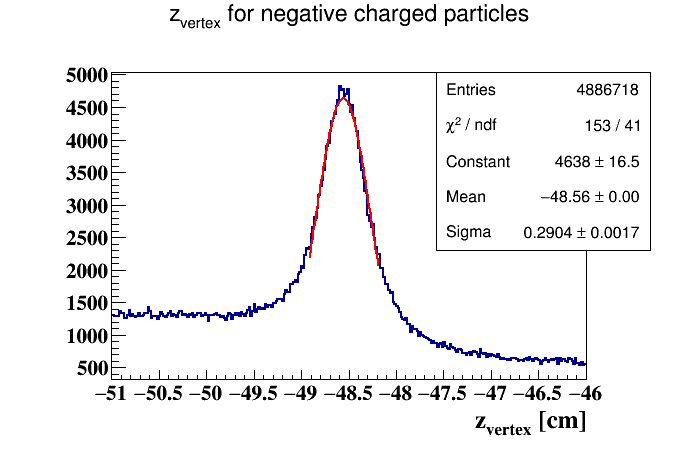
\includegraphics[height=6.2cm]{fig/clas_z_resolution.png}
\caption{ z-vertex of scattered electrons at 6 GeV beam energy from the 
downstream window of the target. The z-vetex resolution of CLAS here is about 3 
mm.}
\label{fig:z_electron_res}
\end{figure}

21) Fig. 2.37: Clearly, momenta are shifted 10$\%$ lower on average. This is 
not surprising, since at low momentum, energy loss will reduce the 
reconstructed radius of the helix. However, since the 4He momentum enters 
various cuts, we need a better understanding of Deltap/p as a function of p and 
theta, e.g. through 2D plots like Figs. 2.11-2.13. Of course it would be even 
better to CORRECT p for energy loss and other effects - but Section 3.3 doesn't 
mention any kinematic corrections for 4He. (I don't insist on this, but the 
effect on the 'true exclusivity' of the final cuts should be discussed.\\  
\textcolor{blue}{We do in fact correct for energy loss. The correction is 
calculated from energy loss in GEANT between the primary electron vertex and
the midpoint of the drift region. This correction was parameterized in terms 
of $(p,\theta)$ and particle type, it was validated by hand-integrating 
Bethe-Bloch formula. The left panel of Figure \ref{fig:energylosscorrection} 
shows our energy correction for a few polar angles. 
The following plots, \ref{fig:delta_p_p} and \ref{fig:delta_p_theta}, 
show that the momentum shift after the energy correction 
as a function of the measured momentum is still present. One could deduce
that our energy loss correction is not strong enough however 
no correlation is observed with the measured polar angle, which
should be expected if the mismatch was due to energy loss. Different
unidentified issues are probably at the origin of this problem.}\\
\textcolor{blue}{We decided to test corrections based on the z-dependence shown
in figure \ref{fig:delta_p_z}. Figure \ref{fig:P_diff_z_correction} shows the 
difference between the elastic 4He momentum and its calculated value 
from the electron scattering 
angle. A second test was performed by doubling the energy loss, which gives 
correct momentum.  When applied on He4 DVCS, as shown in figure 
\ref{fig:dvcs_mom_corr}, we see a deterioration of the missing transverse 
momentum. We conclude that the momentum shift comes from more complicated 
effects linked to angles and possibly other experimental conditions and cannot 
be simply corrected
by a scale factor.}\\

\begin{figure}[tbp]
   \centering
   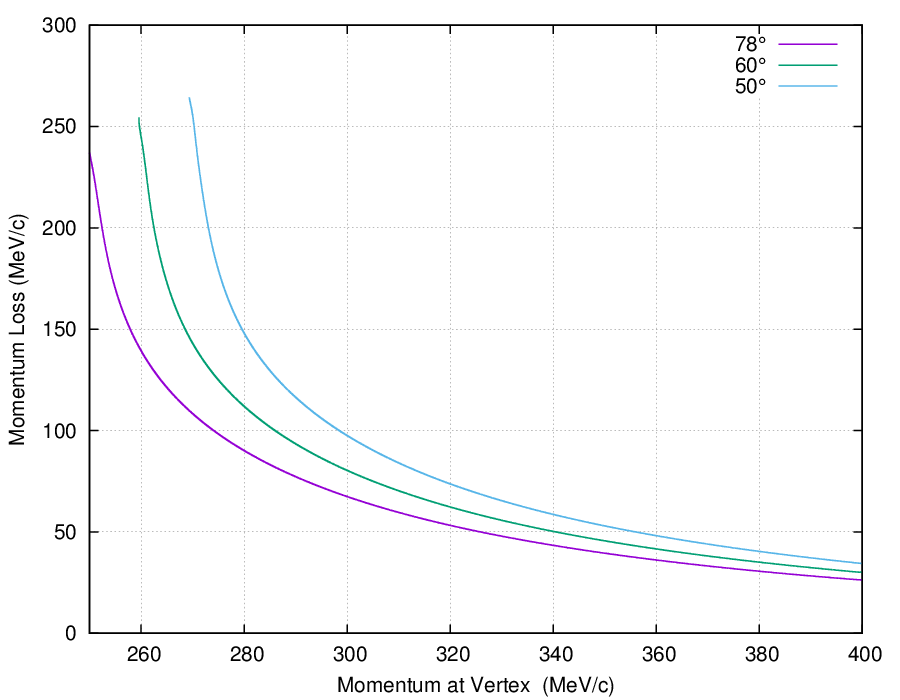
\includegraphics[height=6.2cm]{fig/eg6eloss_4He_rot.png}
   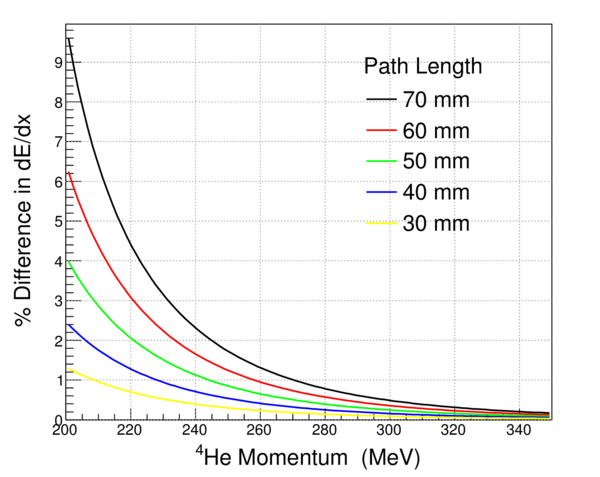
\includegraphics[height=6.2cm]{fig/Biasbb_alpha.png}
   \caption{On the left is the energy loss correction (in terms of momentum)
   derived from full simulation for $^4$He and a few relevant polar angles, where
   the $x$-axis is momentum at the primary vertex.  On the right is the relative
   difference between the instantaneous $^4$He $\frac{dE}{dx}$ at the midpoint of the
   drift region and averaged over the drift region, where the $x$-axis is the average
   momentum in the drift region.  The maximum path length at 40$^\circ$ is about 50 mm.}
   \label{fig:energylosscorrection}
\end{figure}

\begin{figure}[tbp]
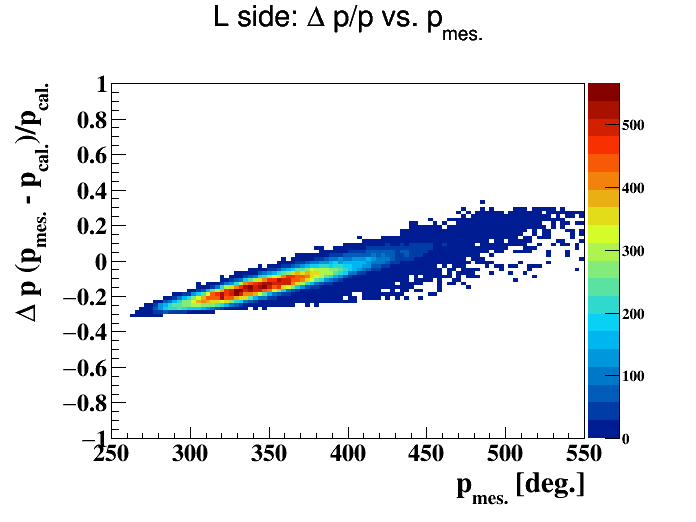
\includegraphics[height=6.2cm]{fig/delta_p_p_elastic_l.png}
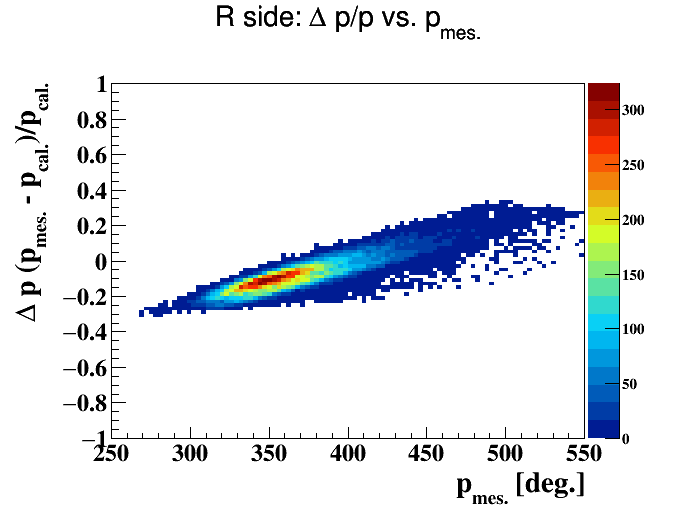
\includegraphics[height=6.2cm]{fig/delta_p_p_elastic_r.png}
\caption{$\Delta$p/p as a function of the p for the identified elastic He4 at 
1.2 GeV electron beam.   }
\label{fig:delta_p_p}
\end{figure}

\begin{figure}[tbp]
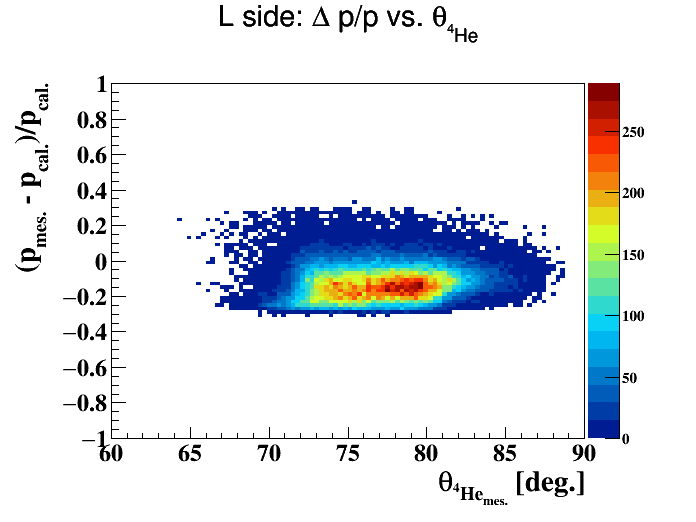
\includegraphics[height=6.2cm]{fig/delta_p_theta_elastic_l.png}
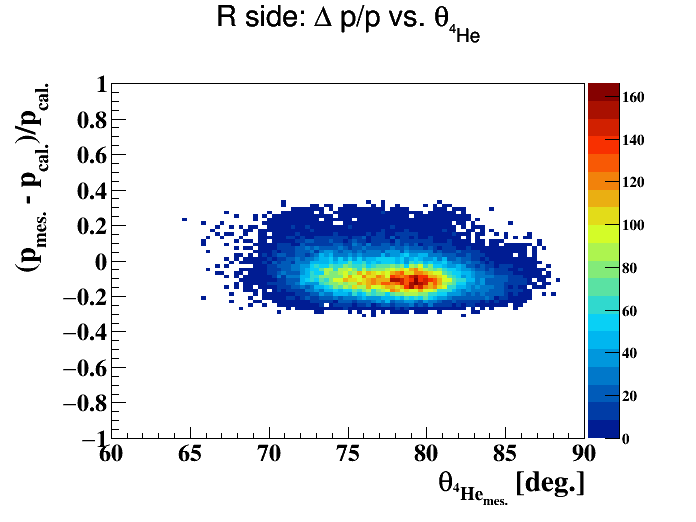
\includegraphics[height=6.2cm]{fig/delta_p_theta_elastic_r.png}
\caption{$\Delta$p/p as a function of $\theta$ for the identified elastic He4.}
\label{fig:delta_p_theta}
\end{figure}

\begin{figure}[tbp]
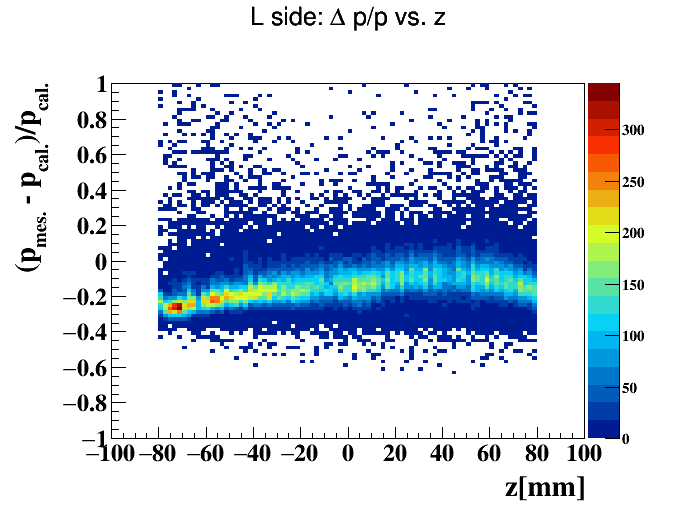
\includegraphics[height=6.2cm]{fig/delta_p_z_elastic_l.png}
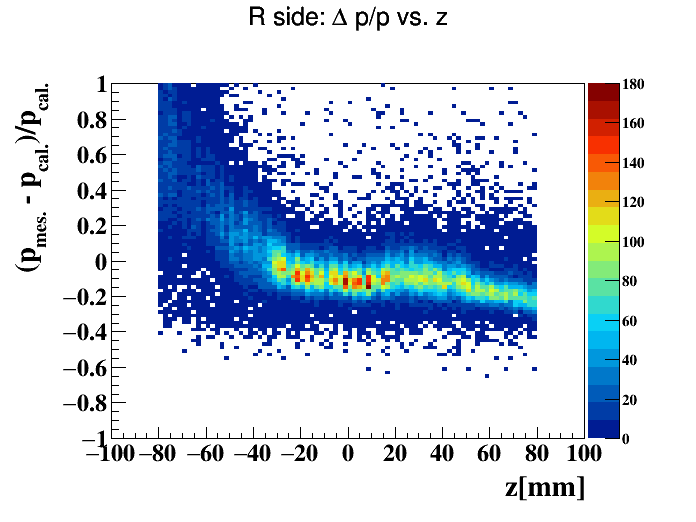
\includegraphics[height=6.2cm]{fig/delta_p_z_elastic_r.png}
\caption{$\Delta$p/p as a function of z-vertex for the identified elastic He4.}
\label{fig:delta_p_z}
\end{figure}

\begin{figure}[tbp]
   \centering
   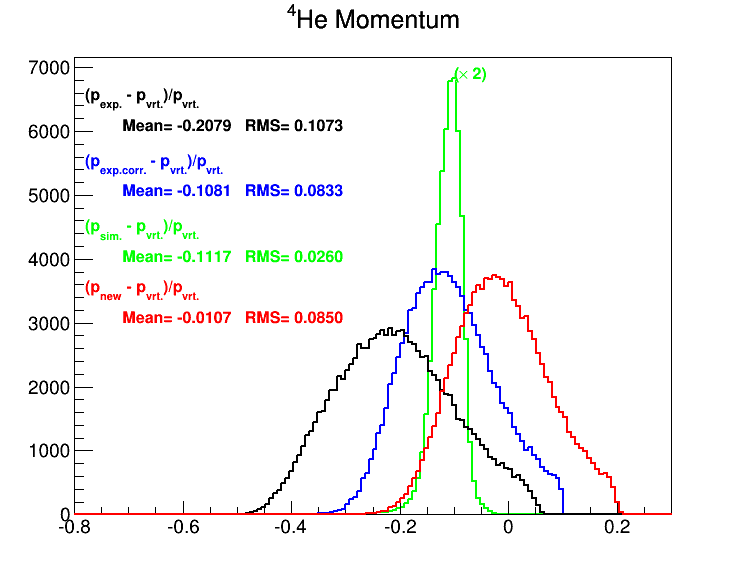
\includegraphics[height=6.2cm]{fig/P_diff_z_correction.png}
   \caption{$\Delta$p/p without any corrections (in black), after energy loss 
   corrections (in blue), from simulation (in green), and after the corrections 
extracted based on the z-dependence (in red) on top of the energy loss 
corrections.}
   \label{fig:P_diff_z_correction}
\end{figure}

\begin{figure}[tbp]
   \centering
   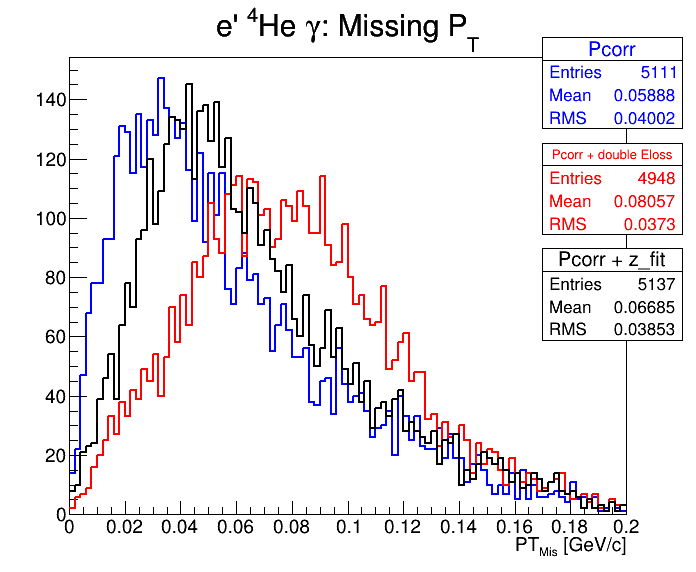
\includegraphics[height=6.2cm]{fig/Coh_e4Hegamma_PT_Mis.png}
   \caption{The missing transverse momentum for the identified coherent DVCS 
      events, after applying only the energy loss corrections (in blue), 
      doubling the energy loss corrections (in black), and after applaying the 
   extracted momentum correction form the z-dependence.}
   \label{fig:dvcs_mom_corr}
\end{figure}

22) Section 3.1: p. 40, 1st bullet: In DIS and SIDIS, the pe cut is supposed to 
remove events with large radiative effects due to photon radiation followed by 
elastic scattering. Here, this is actually part of the signal (interference of 
BH and DVCS). So, the cut should instead be chosen to lie just above the 
hardware trigger threshold of the EC, to avoid fluctuating values for this 
threshold to influence the electron sample.\\
\textcolor{blue}{The explanation in the note is wrong. This cut is applied to 
   eliminate low momentum electrons because during the data acquisition, the EC 
   threshold was set to 200 mV corresponding to electrons having a minimum 
momentum of about 0.7 GeV/c. In this analysis, we applied a conservative cut of 
0.8 GeV/c to be above this threshold.}\\

23) Fig. 3.8: Any explanation for the second 'bump' right above 2 nphe? 
Similarly, the 'green curve' which is really red shows a steep edge, again at 
nphe=2. Are there any other cuts applied before this plot, e.g. exclusivity or 
Osipenko?\\
  \textcolor{blue}{The ``peak'' visible in Figure \ref{fig:nphe_1} above 2 
nphe is the tail of the single photo-electron peak. 
The supression at 1.5 nphe is just an effect of the trigger and creates the 
artificial appearance of a peak just above 2 nphe when only loose cuts are 
applied.}\\

\begin{figure}[tbp]
\centering
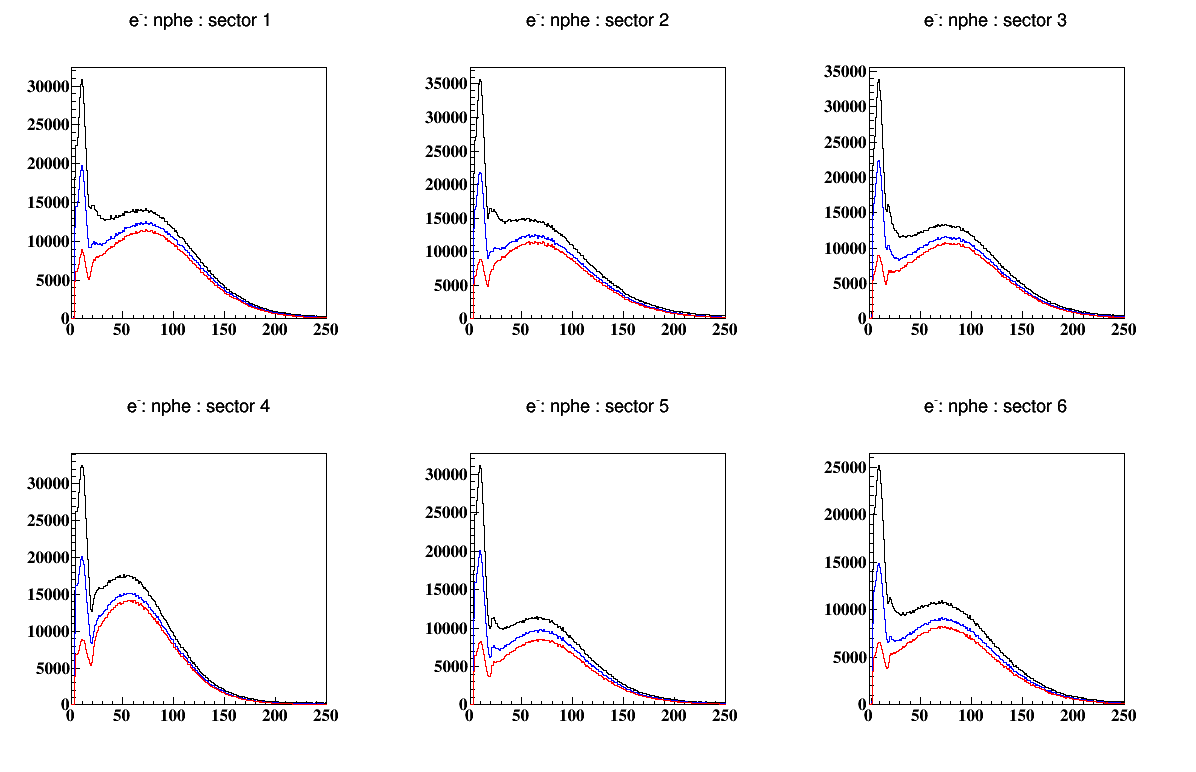
\includegraphics[height=9.2cm]{fig/nphe_1_sectors.png}
\caption{Distribution of nphe emitted by electrons in the six sector of CLAS.}
\label{fig:nphe_1}
\end{figure}

24) Fig. 3.9: Seems superfluous - it doesn't show anything new and doesn't 
contain all the fiducial cuts.\\
 \textcolor{blue}{Removed.}\\

25) p. 45 bottom: Are there any fiducial cuts to remove dead regions? Why 
not?\\
\textcolor{blue}{They are not implemented in this analysis as we deemed them
insignificant for this low statistics asymmetry measurement.}\\

26) Fig. 3.15: This may be my ignorance, but it looks like there is a 
secondary 'bump' between beta =0.9 and 1. What could it be? If it's neutrons, 
wouldn't that contribute to your background?\\
\textcolor{blue}{We seem to disagree there is a significant bump. However, if 
   there are some neutrons, they will be highly suppressed by the DVCS
   exclusivity requirements. In particular we want to point out the energy of the 
   neutral particle is always greater than 2 GeV. At such energies the time 
   of flight measurement from the EC is not good enough to separate neutrons 
   from photons anyway (see Fig. \ref{fig:sim_coh} and \ref{fig:sim_incoh}).}\\

27) Bottom p.47: Indicate that the threshold on IC discris towards TDC has been 
too high to be useful and/or the flight path is too short to apply a beta cut 
as in EC.\\
\textcolor{blue}{
 The timing of the IC is not functionning properly for certain channels. Therefore, 
 applying a timing cut would add inefficient regions in the detector that we 
 wanted to avoid. Moreover, the comment from previous answer applies as well,
such a cut would be very little help to reduce backgrounds at such high particle energies.}\\

28) Fig. 3.19:  The lhs of the RTPC apparently has only 1/2 the efficiency of the 
rhs. Is there any good explanation (at least qualitatively)? This could 
potentially distort $phi$-distributions, no? \\
\textcolor{blue}{ 
   This difference in the yield should not be linked to a different performance 
   of the RTPC.  They are due to the complicated convolution of CLAS and the 
   RTPC acceptance.  We measured the efficiency of RTPC using elastic 
scattering, and found that the left/right halves have similar efficiencies 
except near the upstream and downstream ends, as shown in 
Figure~\ref{fig:tpceff}.} \\

\begin{figure}[tbp]\centering
  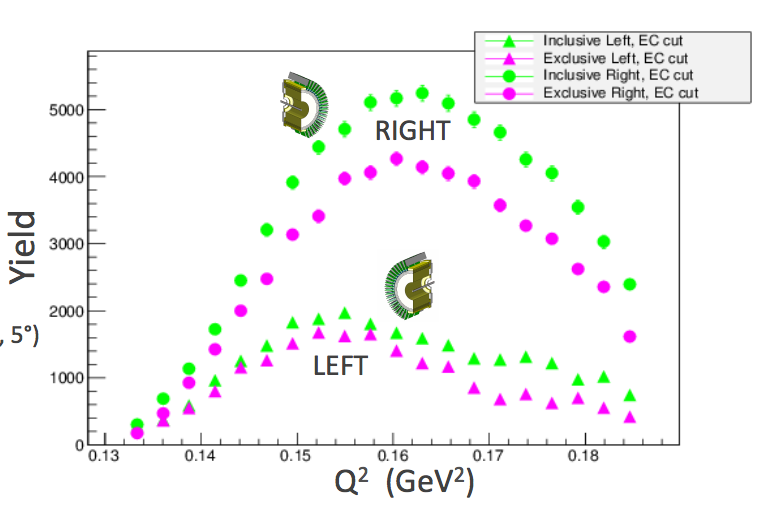
\includegraphics[width=8cm]{fig/tpceffyields.png}
  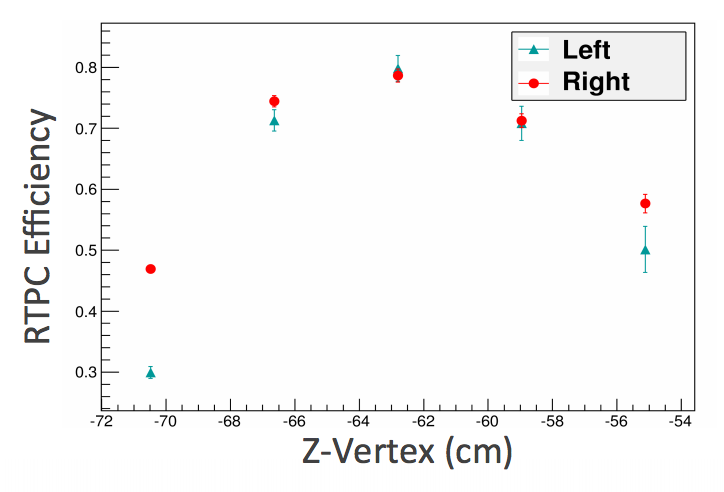
\includegraphics[width=8cm]{fig/tpceff.png}
  \caption{On left is the inclusive and exclusive elastic yields separated into 
     the two RTPC halves (LEFT/RIGHT).  Here the inclusive yields are the 
     number of electrons in the elastic W-peak (e.g.\ Fig.~\ref{fig:W_sec}) 
     whose corresponding elastically scattered $^4$He would have been in the 
     acceptance of the RTPC, and the exclusive yields require the additional 
     detection of the $^4$He.  The large LEFT/RIGHT differences in CLAS 
     acceptance for elastic kinematics are clear in the inclusive yields.  On 
     right is the RTPC $^4$He efficiency calculated from the ratio of exclusive 
     and inclusive elastic yields.  (Here LEFT/RIGHT is from the beam's 
     perspective, i.e.  beam-LEFT/beam-RIGHT)\label{fig:tpceff}}
\end{figure}

29) bulleted list p. 48-49, Bullet 2: Would be nice to see a distribution of 
number of active pads vs. p (but not necessary).\\
\textcolor{blue}{It is added and shown here in Fig. \ref{fig:padnb} as well.}\\

\begin{figure}[tbp]
\centering
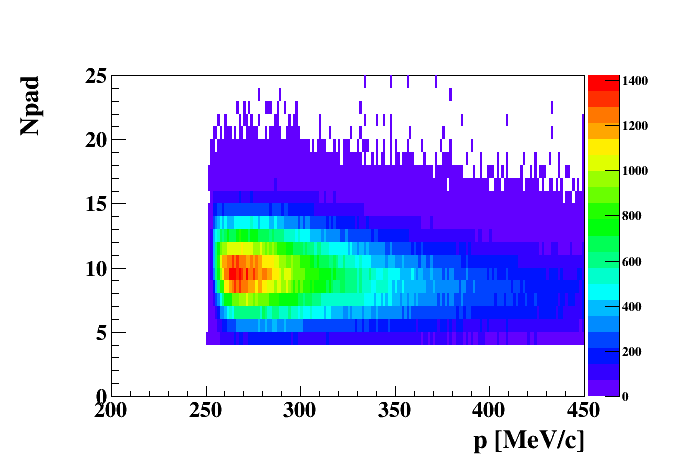
\includegraphics[height=6.2cm]{fig/npd_p_elastic.png}
\caption{The number of active pads versus the measured p for the good tracks 
collected using 6 GeV electron beam.}
\label{fig:padnb}
\end{figure}

30) As asked before: Why is there no PID cut at all? (E.g. Signal height vs.  
p)\\
\textcolor{blue}{We claim that kinematic exclusivity cuts are sufficient to
cleanly select coherent $^4$He DVCS events without the need for $\frac{dE}{dx}$ 
cuts. We performed few checks regarding applying a PID cut, where the full data 
was analyzed in the following three sets:\\
1. Processing all the reconstructed tracks in each event with the exclusivity 
cuts.\\
2. Processing events with only one good track in the RTPC being 
reconstructed.\\
3. Processing events with only one track that passes a dedx cut.\\
The results are shown in figure \ref{fig:all_incoh_exc_cuts} in terms of the 
exclusive variables for the identified coherent DVCS events. One can see that 
applying a PID cut would only change the statistics and not the width of 
distributions. On the other hand, figure 
\ref{fig:coh_alu_PID} shows a comparison between the reconstructed beam-spin 
asymmetries with and without applying a PID cut. The two sets 
of asymmetries are compatible within the given statistical error bars.
From these two observations, we deduce that a PID cut on the Helium would
not reduce any background contribution.}\\

\begin{figure}[tbp]
   \hspace{-0.5cm}
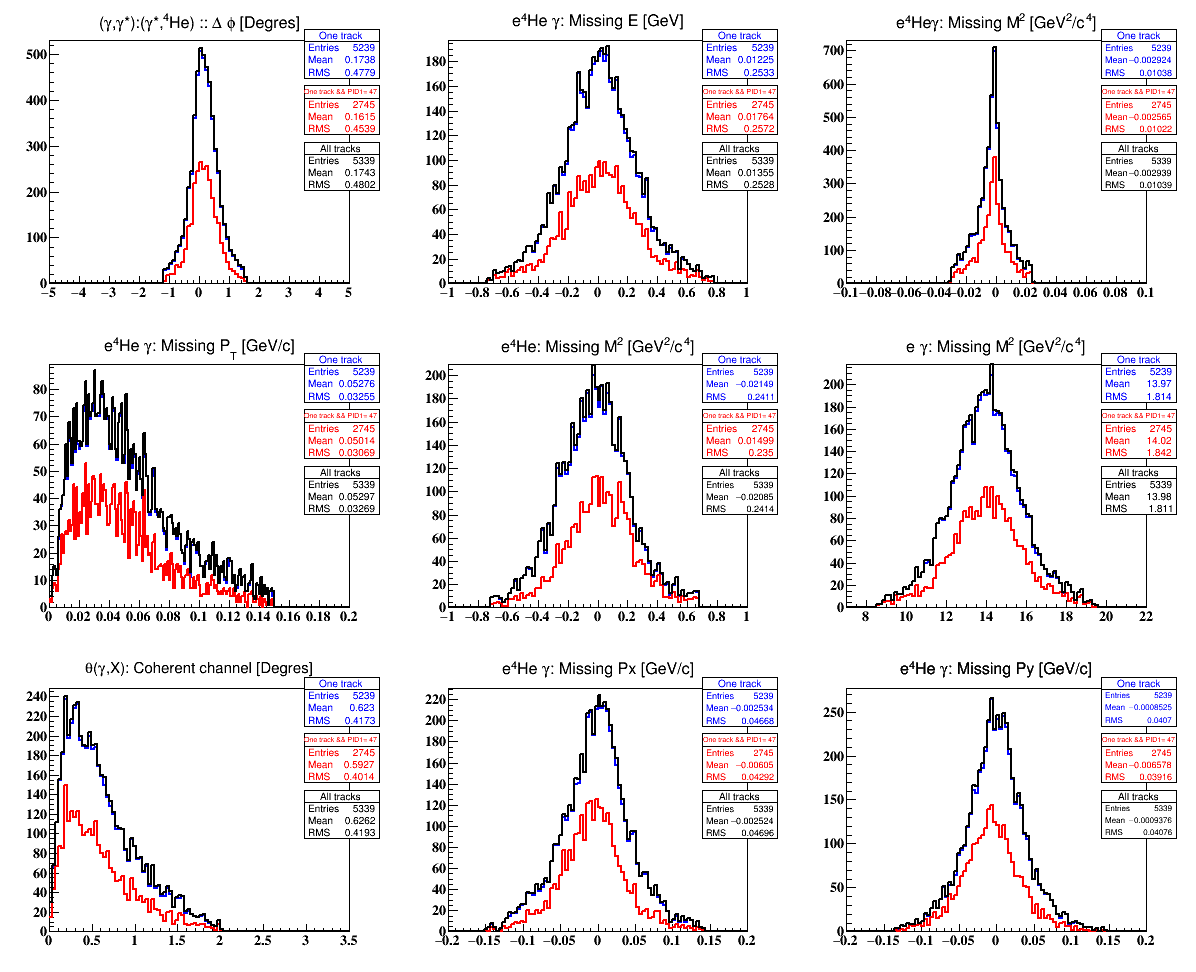
\includegraphics[height=14.2cm]{fig/all_incoh_exc_cuts.png}
\caption{Distributions of the exclusive variable for the identified DVCS events 
with only one track in the RTPC (blue), one track and PID1 is equal to 47 
(red), and processing all the tracks in each event with the exclusivity 
variables (black).}
\label{fig:all_incoh_exc_cuts}
\end{figure}

\begin{figure}[tbp]
   \centering
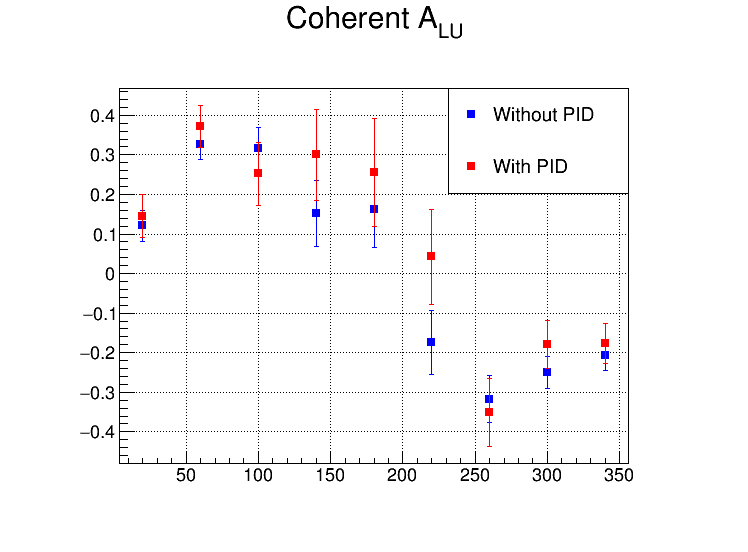
\includegraphics[height=8.2cm]{fig/Coh_ALU_W_out_PID.png}
\caption{The integrated coherent beam-spin asymmetries as a function of 
$\phi$ with (red) and without (blue) applying a PID cut on Helium tracks.}
\label{fig:coh_alu_PID}
\end{figure}


31) Also asked before: What coincidence time window do the $edist$ and $sdist$ 
cuts translate into? This is relevant for accidental coincidences. Fig. 3.23 
indicates clearly that there is an uncorrelated (in z) background from those!  
Yet, there seems to be no discussion of accidental coincidences at all.\\
\textcolor{blue}{For $edist$ and $sdist$ part, it is answered previously in 
comment 6.}\\

\textcolor{blue}{ Regarding the background, figure 
\ref{fig:delta_z_after_exclusitivty} shows $\Delta z$ distributions of the 
identified Coherent DVCS events after applying the exclusivity cuts without any 
initial constrain on $\Delta z$.  This guides us to correct for these 
accidentals in our asymmetries in the form: $ A_{LU~~corr.} = \frac{1}{1 - 
contamination} A_{LU}$, with a 4.1$\%$ global accidental contamination.} \\

\begin{figure}[tbp]
\centering
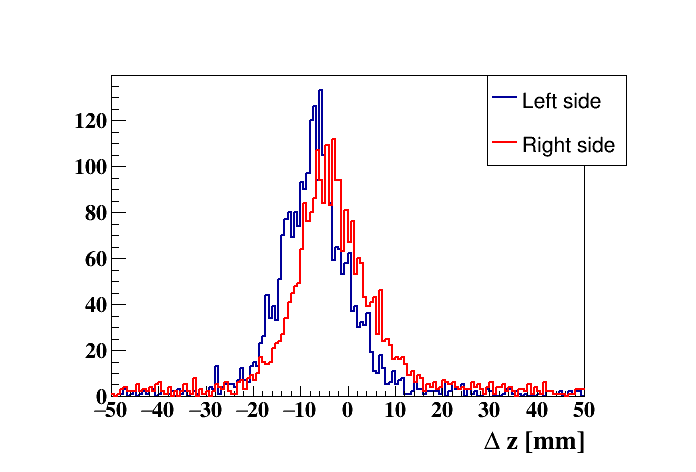
\includegraphics[height=6.2cm]{fig/rtpc_delta_z.png}
\caption{The z-vertex correspondence between the scattered electron and the 
recoil He4 for the identified coherent DVCS events after the exclusivity cuts 
in the two modules of the RTPC separately without any initial constrains on 
z-vertices of the individual particles.  Table \ref{table:Events_numbers} 
summarizes the cut numerically.}

\label{fig:delta_z_after_exclusitivty}
 \end{figure}


\begin{table}[!h]
   \centering
   \begin{center}
      \begin{tabular}{|l|l|l|}
         \hline
         \multicolumn{3}{ |c| }{Number of coherent DVCS events} \\
         \hline
         $\Delta z$ [mm] & Left module & Right module\\
         \hline
         [-50:-30] & 42 & 77 \\
         \hline
         [-20:20]  & 2741 & 2856\\
         \hline
         [30:50]   & 34 &  78 \\
         \hline
         Contamination percentage  & 2.7$\%$  & 5.4$\%$ \\
         \hline 
      \end{tabular}
      \caption{The numbers of the identified coherent DVCS events in the 
      different regions in $\Delta z$ for the two modules of the RTPC.}
      \label{table:Events_numbers}
   \end{center}
\end{table}


32) 3.2: Does the generator contain any kind of implementation for the spectral 
function ('Fermi motion') of the proton in 4He? \\
 \textcolor{blue}{ Yes, the 
Fermi motion is implemented based on the parameterization of  C.~Ciofi~degli 
Atti and S.~Simula (PRC 53 (1996) 1689). Figure \ref{fig:fermi_motion} shows 
the proton initial momentum we used. We cut the high-momentum tail 
at 300 MeV/c, higher momentum should not contribute to the final sample 
because of our exclusivity cuts.} \\

\begin{figure}[tbp]
\centering
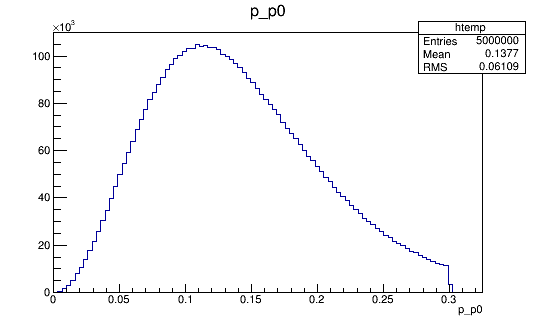
\includegraphics[height=6.2cm]{fig/fermi_momentum_dis.png}
\caption{Fermi momentum distribution for nucleons inside $^{4}$He in GeV/c.}
\label{fig:fermi_motion}
 \end{figure}

 
33) You mention, in 3.2.5, that the RTPC is not implemented in GSIM. Does this 
include the materials as well? If those are not in GSIM, you might 
underestimate multiple scattering and energy loss of electrons and, 
particularly, outgoing protons.\\
\textcolor{blue}{No the material of the RTPC is implemented in GSIM,
however it is only considered as dead material and the detection 
simulation is not implemented. The description is clarified in the
note.} \\


34) Also in 3.2.5, I would like a little more detail on the fastmc: How does it 
calculate the energy loss of the 4He? Is multiple scattering included? Could 
you show comparisons between measured and simulated distributions?\\
\textcolor{blue}{We do not specifically apply energy loss and multiple 
scattering in our fastmc, but we apply resolution effects based on 
experimental data that include both effects. The plots in Fig.~\ref{fig:comp_He} 
show the comparison between data and simulation in terms of theta, $phi$ and 
momentum of the He-4 DVCS nuclei.}\\

\begin{figure}[!h]
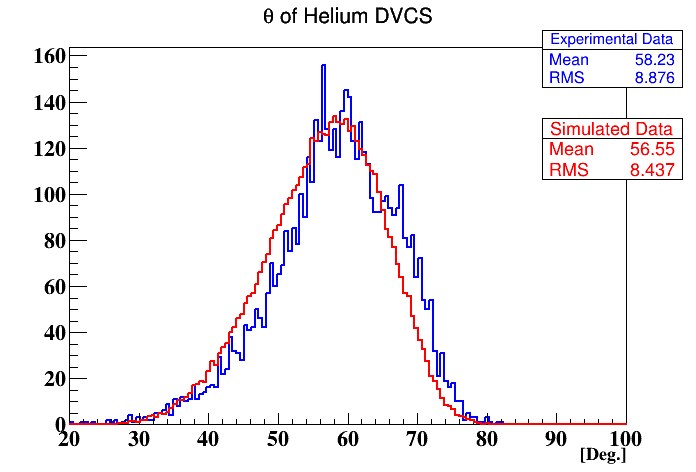
\includegraphics[height=5.0cm]{fig/He_theta.png}
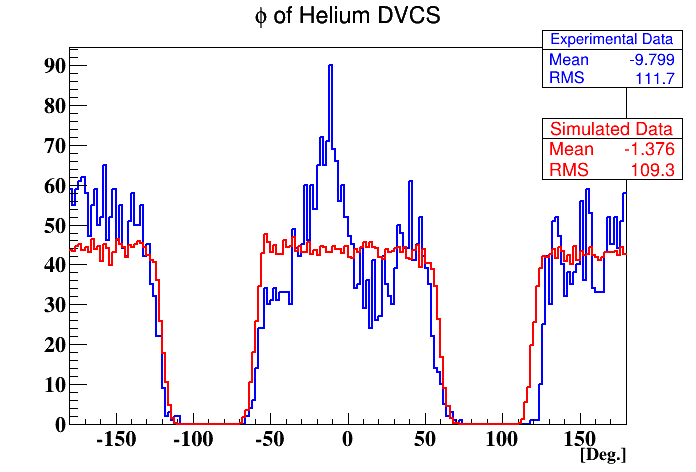
\includegraphics[height=5.0cm]{fig/He_phi.png}
\centering
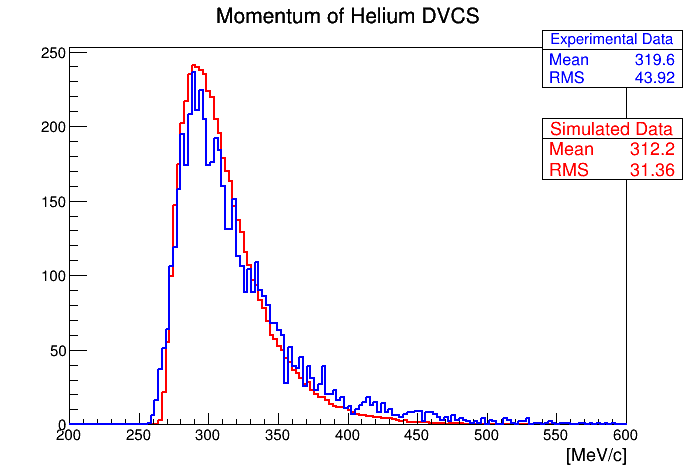
\includegraphics[height=5.0cm]{fig/He_mom.png}
\caption{Comparison between experimental and simulated DVCS $^{4}$He nuclei in 
terms of polar angle, azimuthal angle and momentum.}
\label{fig:comp_He}
\end{figure}

35) 3.3.: The kinematic corrections you mention are based on simulation only and 
mostly take care of energy loss by the protons. Most other CLAS analyses 
require additional, EMPIRICAL kinematic corrections (see, e.g. the BONuS 
experiment). Can you give a justification for leaving them out?
It may be obvious, but you don't show or say it: Are the corrections explained 
in 3.3.1-3.3.3 applied to the real data as well?\\
\textcolor{blue}{For electrons and protons, the presented corrections in 
sections 3.3.1 and 3.3.2, respectively, are applied for experimental data and 
simulation. We did not find the need for additional kinematic corrections on 
protons and electron as we found good enough match already.
In the case of the energy of the IC photons, the corrections 
for data and for simulation are different and presented in the following two 
sections, sections 3.3.3 and 3.3.4. In the latter case
these where empirical corrections.  Additional corrections are not pursued
for the data since data and simulation already agree reasonably well regarding
the quantities that are involved in event selection and asymmetry 
extraction.}\\

36) 3.3.4: The 3 corrections you describe for IC photons are somewhat 
correlated, since they all are checked by optimizing $m_{\pi^0}$. Did you try a 
simultaneous fit of all parameters (or at least several ones) that enter the 
various corrections?\\
\textcolor{blue}{The position correction (3.3.4.2) is derived based on minimizing
$z$-dependence of $m_{\pi^0}$, and is highly uncorrelated with energy 
corrections. The run-dependence (3.3.4.1) is also uncorrelated with energy, as
can be seen in the top panel of Fig 3.35, but is primarily a run-dependent global
scale factor on energy. Finally the radial- and energy- dependent energy correction
(3.3.4.3) are indeed correlated and therefore treated multidimensionally ($R,E$).}\\

37) Fig. 3.39, I am a bit troubled by the huge shift in missing energy - on 
average several 100 MeV - after applying the corrections. This contrasts to  
Figs. 3.34-3.38, where most deviations from the true pi0 mass appear to be less  
than a couple $\%$.\\
\textcolor{blue}{Most $\pi^0$ are found at low energy, while the correction affects
2 to 6.0 GeV photons. This is the reason the correction has such an important 
impact. See later reply to question 31 ii from reviewer 2 for more details.}\\

38) Sec.4.1, Fig. 4.1 and 4.2, Fig. 4.5: In addition to looking at He4/e and 
p/e, why don't you also look at e/FC to eliminate unstable runs?\\
\textcolor{blue}{We did not use the Faraday cup reading in the analysis. We
feel it is an unecessary cut for an assymetry measurement.}\\

Do we have an idea why the RTPC lost nearly 50$\%$ of its efficiency over the 
course of the experiment?\\
\textcolor{blue}{
 This is mainly related to experimental changes in the RTPC. In particular, we 
had leaks in our gas system that appeared during the run. This probably
caused gas contamination, changing the properties of the detector.}\\


39) Eq. 4.1: It would be nice to know the typical value (or range) for tmin.\\
\textcolor{blue}{We show in figure \ref{fig:tmin_both}, for both DVCS 
channels, $t_{min}$ distributions for our DVCS events.}\\

\begin{figure}[tbp]
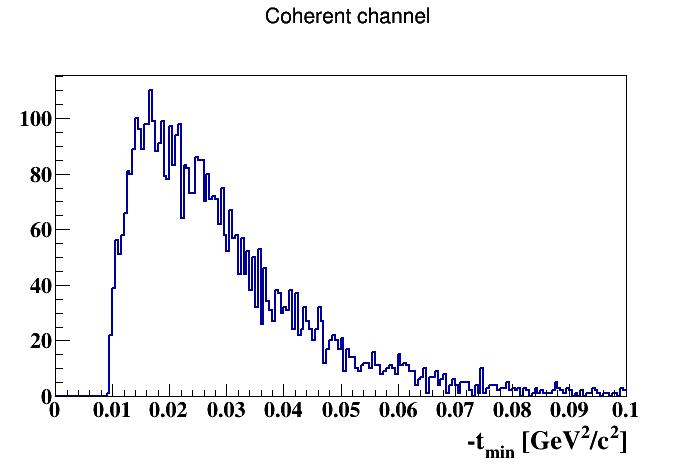
\includegraphics[height=5.0cm]{fig/tmin_coh.png}
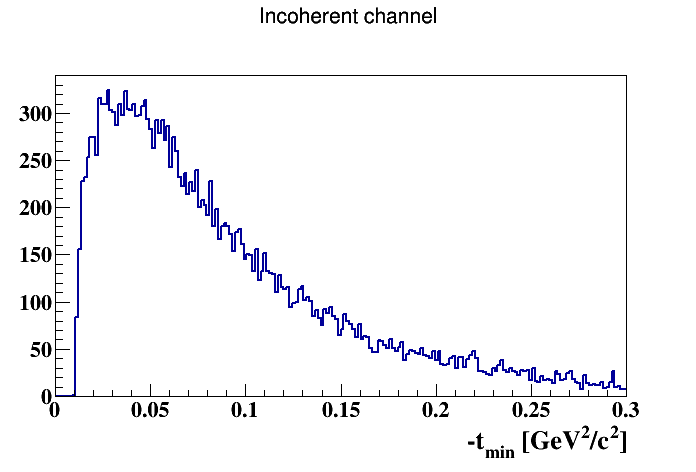
\includegraphics[height=5.0cm]{fig/tmin_incoh.png}
\caption{Coherent (left) and incoherent (right) tmin distributions calculated 
for the experimentally selected DVCS events. We use the experimental $Q^{2}$ 
and $x_{B}$ of the individual events. }
\label{fig:tmin_both}
 \end{figure}


40) Fig. 4.2: I'm bothered by the wide distribution in Emiss (top middle), and 
don't understand why you use such wide cuts. Surely, anything above Emiss = 0.4 
must have additional particles in it, and even if not, why not cut this tail?  
Note that the same tail is absent for the p (FIg. 4.6) where you use indeed a 
tighter cut, although you don't even account for the proton's initial 
momentum.\\
\textcolor{blue}{ We applied 3$\sigma$ based on the comparison between data 
and simulation, see figure 4.4 in the note. In the following, figure 
\ref{fig:coherent_ME_bins}, we performed bins in the missing energy 
distribution and we watch the reconstructed beam-spin asymmetries. As a 
conclusion, we see that the reconstructed asymmetries are compatible within the 
given error bars.} \\

\begin{figure}[tbp]
   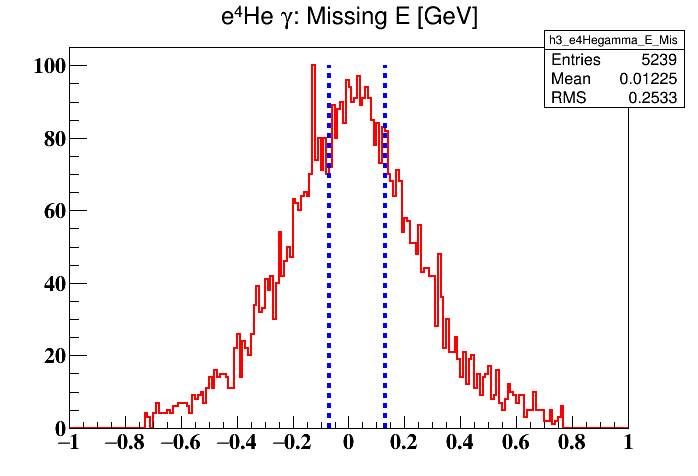
\includegraphics[height=5.0cm]{fig/coh_ME_bins.png}
   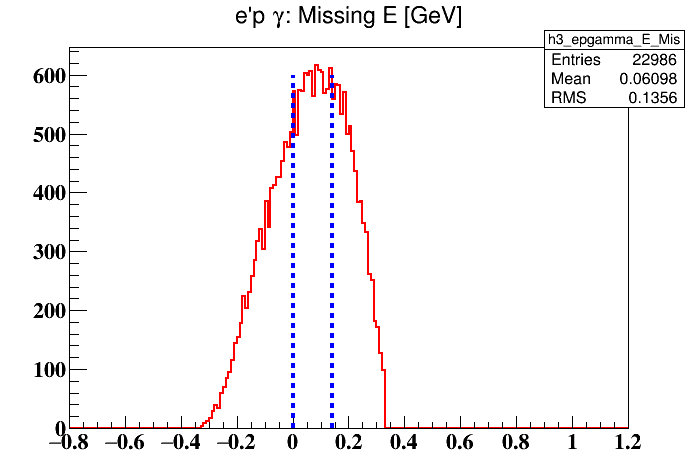
\includegraphics[height=5.0cm]{fig/incoh_ME_bins.png}
   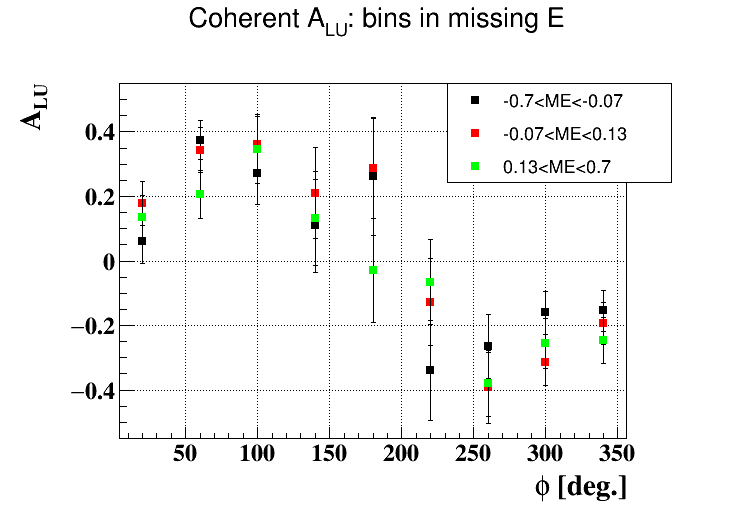
\includegraphics[height=5.5cm]{fig/BSA_coherent_ME.png}
   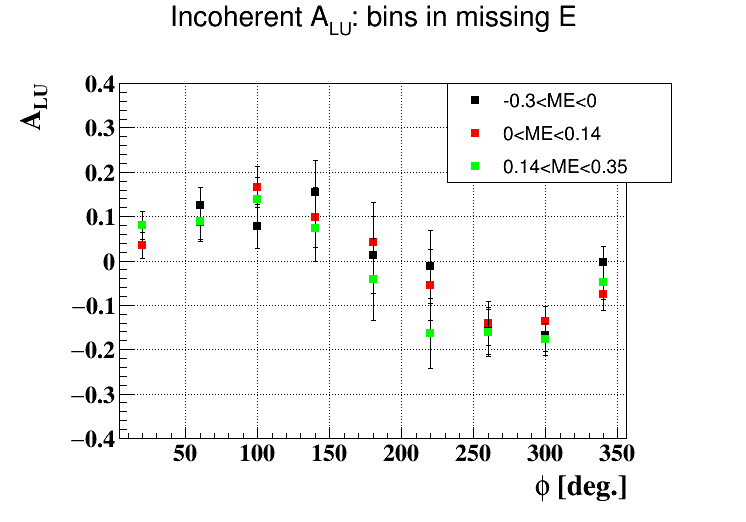
\includegraphics[height=5.5cm]{fig/BSA_incoherent_ME.png}
   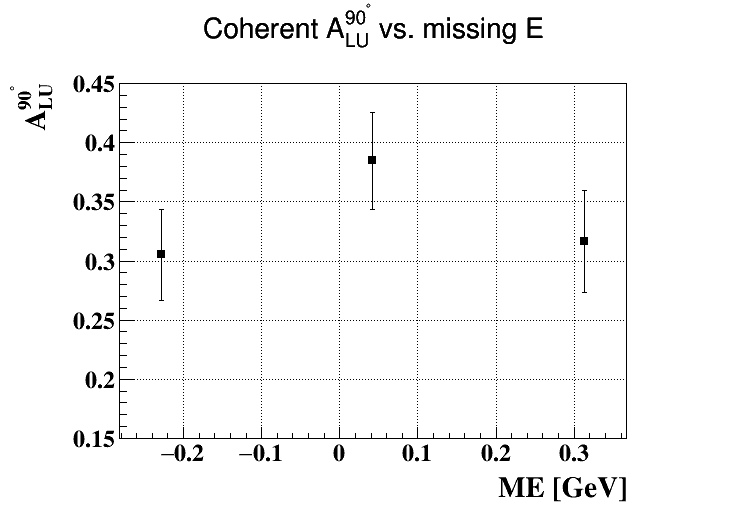
\includegraphics[height=5.5cm]{fig/coh_ME_alpha.png}
   \hspace{+0.7cm}
   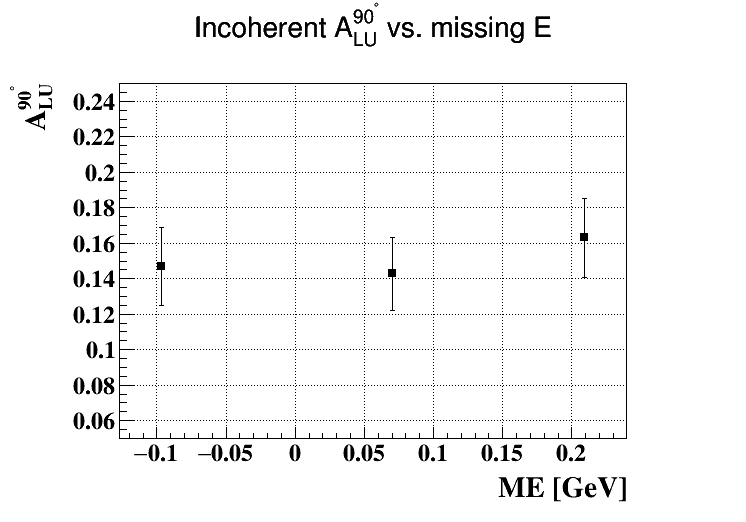
\includegraphics[height=5.5cm]{fig/incoh_ME_alpha.png}


   \caption{Coherent (left) and incoherent (right) missing energy distributions 
   (top), the reconstructed beam-spin asymmetries as a function of $\phi$ 
(middle), and the extracted asymmetry at $\phi = 90 ^{\circ}$ from fitting the 
asymmetries as a function of the missing energy in each bin. }
   \label{fig:coherent_ME_bins}
    \end{figure}

41) Fig. 4.6: Here you could cut deeper on the ep missing mass.
Why is it so lopsided? Didn't you correct the IC photons to avoid that?  \\
\textcolor{blue}{We can always cut deeper. We choose not to cut by eye, but 
   using 3 $\sigma$ in order to avoid biassed choices. Moreover, most 
   contamination eventually remaining is pi0 and is treated by a specific 
correction. We do not understand how IC correction can possibly affect the epX 
system.}\\

42) Fig. 4.8: Again, the missing energy from epgamma is lopsided, as is the 
missing egamma mass. Looks like Egamma is still not properly calibrated; but 
then why are the corresponding plots for the coherent channel spot-on? \\
\textcolor{blue}{The assymetry effects are due to the background of the pi0
contributing only on one side of distributions. The peaks are indeed all 
slightly shifted, this is probably due to a complex mix of misalinements and 
miscalibrations. Any attempt to correct with a simple function for one 
variable makes the other worse. In particular, we want to point out that both 
epX and e$\gamma$X missing mass are slightly off but ep$\gamma$ missing mass 
is peaked at 0. These problem do not appear for the coherent channel because
of the larger mass term that reduce the relative impact of some of the
measurement errors. Equation \ref{eq:egamma} shows that the precision on the 
calculated missing mass squared of $e\gamma X$ depends on the mass of the 
initial state hadron in each DVCS channel.}\\
   \begin{equation}
      \frac{\partial MM^2_{e\gamma X}}{\partial E_{\gamma}}
      = 2*(E_{\gamma^{*}}-M_{target} - E_{\gamma})
      \label{eq:egamma}
   \end{equation}

43) 4.5: You discuss the pi0 background. Am I correct to assume that Eq. 4.11 
is applied separately for each beam helicity? (I assume you use the same R, but 
of course the reconstructed pi0 events could - probably will - have an 
asymmetry).   \\
\textcolor{blue}{Yes, the subtraction is done separately for each helicity 
   direction. We modified the text to include that information. As can be seen 
   from figure \ref{fig:pi0yield}, the $\pi^0$-background yield with respect to 
   the coherent DVCS events is around 2-4$\%$.}\\
   \textcolor{blue}{
   Figure \ref{fig:coh_dvcs_pi0_Alu} shows the reconstructed coherent 
   asymmetries in t-bins as a function of $phi$, where the red shaded point are 
   the DVCS asymmetries after the background subtraction, the blue points are 
   the DVCS raw asymmetries without background subtraction and the black points 
   are the $\pi^0$-asymmetries ($e^{4}He\pi^{0}$ events).  }\\
\textcolor{blue}{This leads us to conclude that:\\
- The  $\pi^{0}$-asymmetries are consistent with zero.\\
- 2-4$\%$ background yield does not affect much our DVCS asymmetries.\\
Therefore, assuming that the two helicity configuration have the same 
acceptance ratio R is a good approximation.}\\

\begin{figure}[tbp]
   \centering
   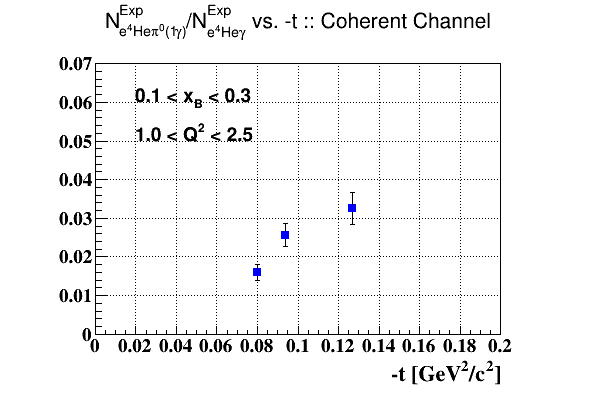
\includegraphics[height=5.5cm]{fig/t_ratio_coh_t.png}
   \caption{The coherent $pi0$-background yield.}
   \label{fig:pi0yield}
\end{figure}
                          
\begin{figure}[tbp]
   \centering
   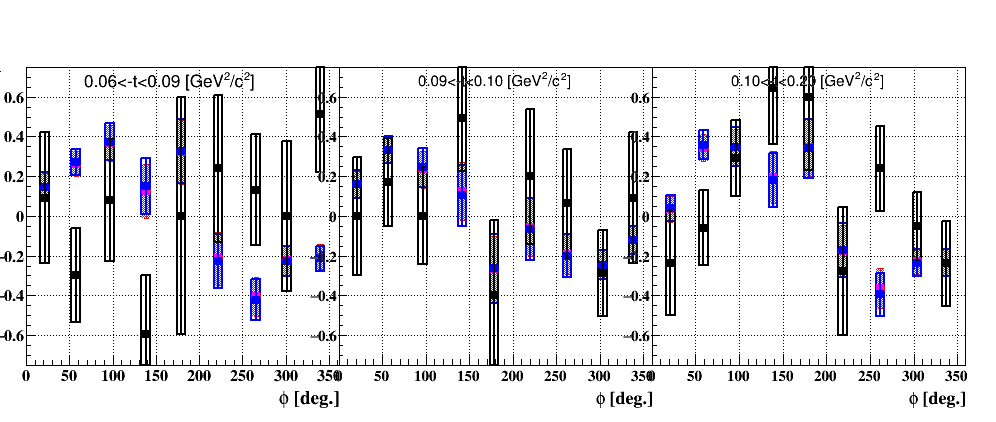
\includegraphics[height=7.5cm]{fig/coherent_AlU_pi0.png}
   \caption{In black, measured coherent $\pi^{0}$ asymmetries. In blue, the 
   coherent DVCS asymmetries without background subtraction. In red: the 
coherent DVCS asymmetries after the background subtraction.}
   \label{fig:coh_dvcs_pi0_Alu}
    \end{figure}


 
44)Unfortunately, no other backgrounds are discussed (not even dismissed): 
scattering from other target components (Kapton? windows?), events with more 
particles in the final state (especially since you allow such a large Emiss), 
and accidental coincidences (particular for the coherent channel), plus perhaps 
photon misidentification. The various strange 'bumps' I've pointed out along 
the way show that those backgrounds may not be totally negligible. \\
\textcolor{blue}{The procedure follows the same guidelines as for DVCS 
analysis on the nucleon. The neutral pion production occurs "without threshold" 
as seen from the $eHe\gamma$ sample, meaning that the contamination from 
$eHe\pi^0$ with one photon lost is distributed all the way down to the DVCS, 
in the limit where the second photon energy becomes negligible in 
the lab. Single charged pion production occurs with a small threshold but is 
inconsistent with the already detected particles (e and He). Two pion 
production is entirely cleaned up by the exclusivity cuts. Scattering from the 
windows is excluded by the vertex cuts. As far as accidental, we correct for 
that as presented in comment \#31 from the first reviewer. For discussions of 
other background sources see also the answers to:\\
- Comment 46, figure 30, from the first reviewer.\\
- Comment 7, figure 47, from the third reviewer.\\
- comment 14, figure 52, from the third reviewer.}\\


45) Fig. 4.11: For the final correction, do you produce the $phi$-dependence of R 
for each of the individual bins in xB, Q2 or t that you use? \\
 \textcolor{blue}{Yes we do.}\\

46) 4.7: I admit to being biased and a pain in the butt about this, but I NEVER 
understand why more or less arbitrarily varying a cut (and, in this case, even 
a rather meaningless cut in my mind) gives you a QUANTITATIVE estimate of 
background uncertainties. For one, you are mixing systematic effects from the 
tails with statistics (since you change the sample size). Plus, how do you know 
that there isn't even sizable background for your smallest (2.0 sigma) 
variation? I'd much rather see a sequential, quantitative discussion of 
possible background sources and direct estimates of their magnitude INSIDE all 
cuts (e.g., by selecting background events on purpose and looking at their 
distribution in the variables that you cut on). See above for a list of such 
backgrounds.\\
 \textcolor{blue}{Cuts are arbitrary, we could choose 2.32 sigma or 2.74 and 
there is no strong argument for either. It is therefore necessary to associate
an error with this choice. The chosen variable (missing mass of ep$\gamma$) is 
neither meaningless nor arbitrary, it is the one with the larger tails even 
after applying all other cuts. From these, it seems clear that such a study 
indicates a clear source of systematic errors linked to background. It can of 
course be argued that this test does not account for the full background error, 
but we never claimed this, so we are unsure what is the source of the critic. In 
fact, we claim the opposite since we treat $\pi^0$ background independently and 
associate another systematic error to it.}\\

 \textcolor{blue}{ Regarding the windows effect inside the exclusive 
    distributions, the data has been processed with NO constraints on the 
    z-vertex of the electron nor the $^{4}$He. Figure \ref{fig:exclusive_z} 
    shows the exclusive variables as a function of z-vertex of the electron for 
 the identified coherent DVCS events. The target extends from -74 cm to -54 cm 
 with respect to the center of CLAS. As a conclusion, our vertex cut, shown in 
 figure 3.1 in the note, remove most of the windows effect. For the remaining 
 contamination, we correct for it as presented in comment 44 from the first 
 reviewer. }\\

 \begin{figure}[tbp]
 \centering
 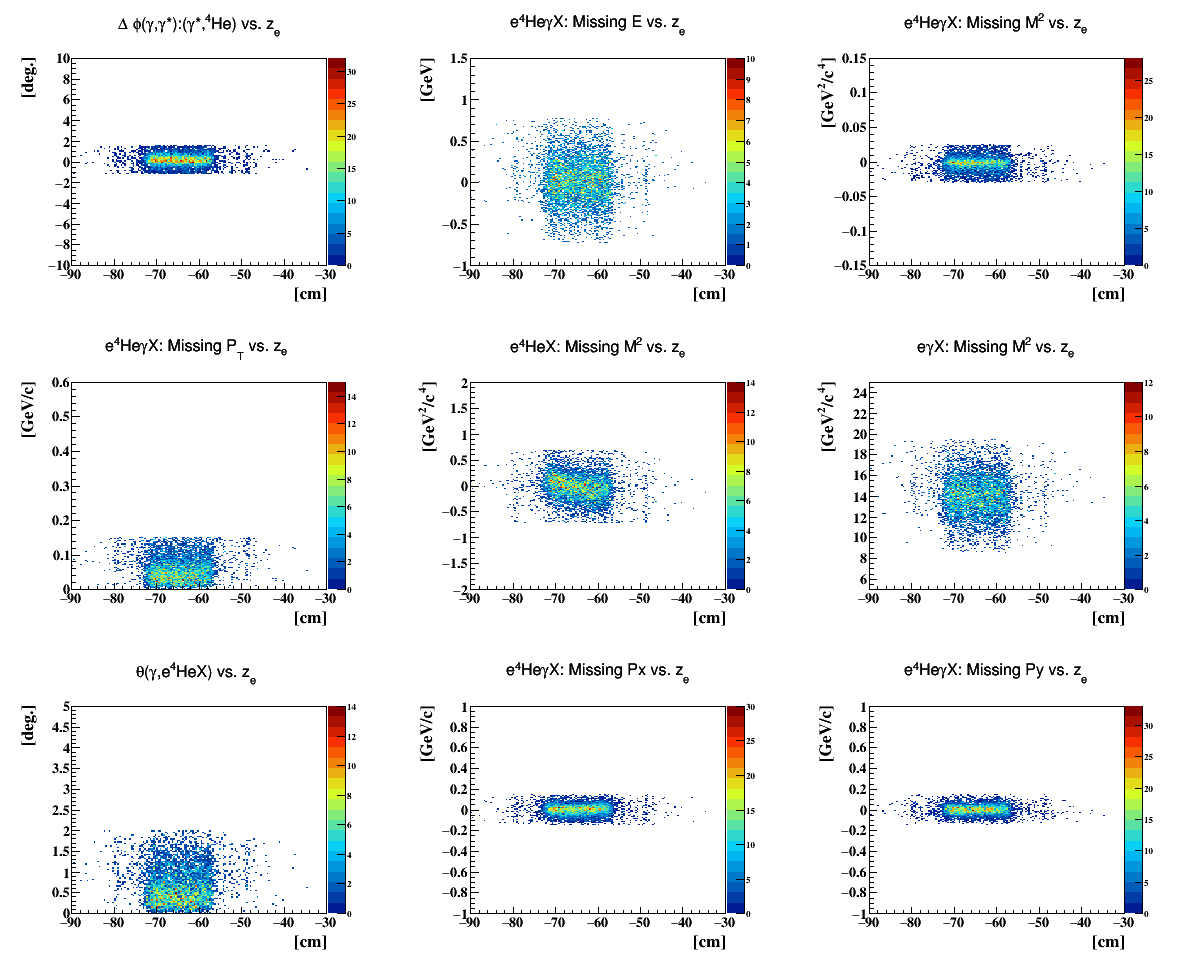
\includegraphics[height=14.5cm]{fig/exclusivity_zele.png}
 \caption{The distributions of the exclusive variables as a function of 
 z-vertex of the scattered electron after applying all the exclusivity cuts 
 without any initial constrains on $\Delta z$ nor the z-vertices of the 
 individual particles.}
 \label{fig:exclusive_z}
 \end{figure}


47) p. 80: I believe that one-loop corrections aren't a big worry. However, one 
contribution I can think of is the radiation of a second photon, e.g. right 
before the actual DVCS event (and not connected to a pi0). It's not clear to me 
that this is a priori a small effect, again especially given the wide Emiss 
cuts. \\
\textcolor{blue}{It has been shown that such effects are small for asymmetries
on free proton and we see no argument to claim otherwise. Actually reviewer 2
in its question 41 is supporting this point.}\\

48) Fig. 5.2: 'red error bars' aren't visible - use shaded bands instead.
    To do, unbinned fit and separate the systematic errors. \\
    \textcolor{blue}{In figures \ref{fig:coh_alu_sep} and 
       \ref{fig:incoh_alu_sep} we show the coherent and the incoherent 
    beam-spin asymmetries respectively. In blue the statistical and the 
 systematic errors are added quadratically, in green the statistical errors and 
 brown bands present the full systematic uncertainties. The red lines are fits 
 to the data and presented in chapter 5 of the note. } \\
 \begin{figure}[tbp]
 \centering
 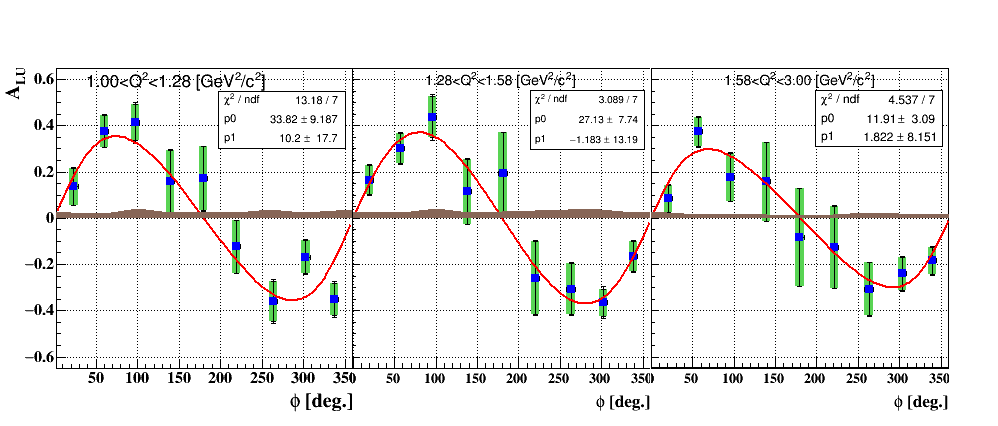
\includegraphics[height=7.0cm]{fig/coh_Q2_phi.png}
 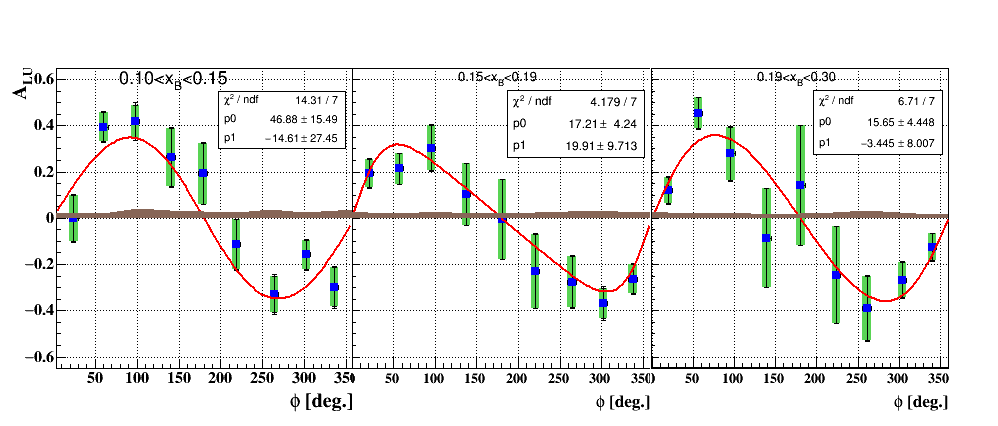
\includegraphics[height=7.0cm]{fig/coh_xB_phi.png}
 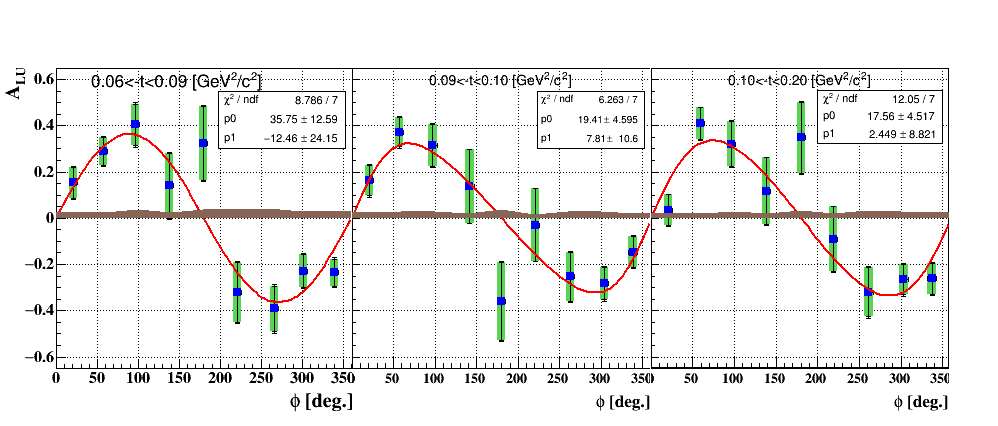
\includegraphics[height=7.0cm]{fig/coh_t_phi.png}
 \caption{Coherent beam-spin asymmetries}
 \label{fig:coh_alu_sep}
 \end{figure}

 \begin{figure}[tbp]
 \centering
 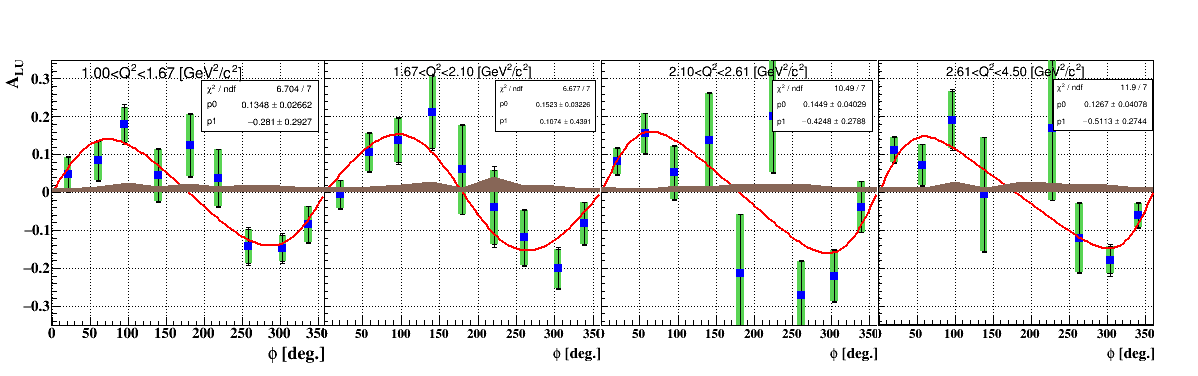
\includegraphics[height=5.5cm]{fig/incoh_Q2_phi.png}
 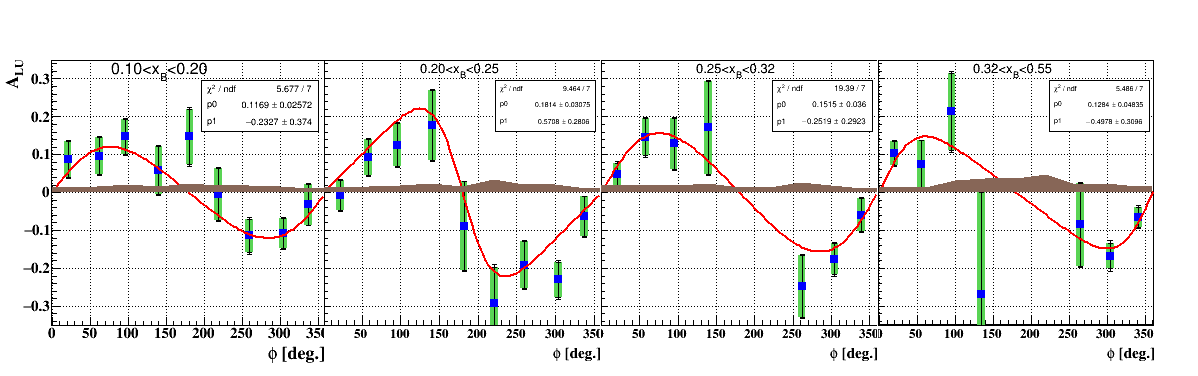
\includegraphics[height=5.5cm]{fig/incoh_xB_phi.png}
 \includegraphics[height=5.5cm]{fig/incoh_t_phi.png}
 \caption{Incoherent beam-spin asymmetries}
 \label{fig:incoh_alu_sep}
 \end{figure}



49) Fig. 5.3: Why the weird vertical ticks and tick labels? At least 0 should 
be clearly marked. Also, indicate the averages of the 2 other variables in the 
same way in the 3 plots, indicating that it is an average? \\
\textcolor{blue}{It is corrected in the second version of the analysis note, 
see figures 5.2 and 5.4.} \\

50) Fig. 5.5: Are the curves integrated over the experimental acceptance? 
Again, showing averages for all 3 variables (preferably for each data point) 
would help interpret the applicability of the curves.
- No matter what, you must supply tables for all your ALU(90deg) results with 
averages of all kinematic variables for each data point - after all, there 
aren't so many. \\
\textcolor{blue}{The theoretical curves are not integrated over the 
   experimental acceptance. For example, they are calculated at fixed xb, Q2 
   and $phi$ when looking to the dependence on t. Tables for all the two 
   dimensional bins are added to the note for both the coherent and the 
   incoherent channel as well as at the end of this document in tables 
   \ref{table:Coh_Q2_BSA} to \ref{table:InCoh_t_BSA}.  
} \\  

51) Fig. 5.6: It would be nice to superimpose the incoherent p results from 4He 
on the same graphs.\\
\textcolor{blue}{ Figures 5.4 and 5.6 are superimposed in figure
\ref{fig:incoh_free_ALU}}
\begin{figure}[tbp]

   \includegraphics[height=5.5cm]{fig/Q2_dep.png}
   \includegraphics[height=5.5cm]{fig/xB_dep.png}
   \includegraphics[height=5.5cm]{fig/t_dep.png}
   \caption{The blue (black) points are the incoherent (free) proton $A_{LU}$ 
   as a function of $\phi$ in $Q^{2}$, $x_{B}$ and $-t$ bins.}
   \label{fig:incoh_free_ALU}
\end{figure}
\\

52) Fig. 5.7: I'm confused why Im(HA) is rising with Q2 but falling with xB.  
These 2 are pretty tightly correlated! Any explanation?\\
\textcolor{blue}{The new extraction of the GPDs show almost the same trend in 
   $Q^2$ and $x_B$, where the data is fitted with a form in which the real and 
   the imaginaries parts of the CFF $H_A$ are the free parameters. The previous 
   observation might come for the neglecting some parts of the full formula 
that we thought would be negligible. } \\

53) 5.4: 3rd paragraph: Be careful not to over interpret the meaning of your 
results. For one, your xB is more closely related to xi, not x in DIS. Also, 
there are other possibilities to explain the smaller asymmetries for bound 
protons than the EMC effect - e.g., FSI. \\
\textcolor{blue}{We are not sure what you are referring to. We clarified a 
little the paragraph in order to alleviate any issues.} \\
\textcolor{blue}{Regarding the FSI effect, this can be investigated by 
construction bins in missing transverse momentum. Figure 
\ref{fig:alu_alpha_bins_pt} shows the extracted $A_{LU}$ at 90$^{\circ}$ from 
fitting the asymmetry signals for different $p_t$ bins. As a conclusion one 
can see that the incoherent asymmetries are consistent and so the FSI seem to 
have no big effects on the measured asymmetries. This question of course is to 
be discussed in more detail in the paper, rather than in the analysis note.}\\

%\begin{figure}[tbp]
% \centering
% \includegraphics[height=5.5cm]{fig/incoh_bins_pt.png}
% \caption{ Three reconstructed bins in the missing transverse momentum.}
% \label{fig:bins_pt_incoh}
%\end{figure}

%\begin{figure}[tbp]
% \centering
% \includegraphics[height=6.5cm]{fig/BSA_incoherent_PT.png}
% \caption{The reconstructed beam-spin asymmetries as a function of $phi$ in the 
% for the bins shown in figure \ref{fig:bins_pt_incoh}.}
% \label{fig:incoh_Alu_pt}
%\end{figure}

 \begin{figure}[tbp]
  \centering
  \includegraphics[height=6.5cm]{fig/incoh_PT_alpha.png}
  \caption{The incoherent beam-spin asymmetries at $\phi = 90 ^{\circ}$, from 
  fitting the signals, as a function of the missing pt.}
  \label{fig:alu_alpha_bins_pt}
 \end{figure}

54) 4th paragraph: I am not sure what you are saying with 'in the same coherent 
domains of ...'. Can you specify exactly which range in x, t and Q2 either data 
set is integrated over?\\
\textcolor{blue}{We modified the text to include that information. }\\

55) Fig. 5.9: Certainly interesting, but maybe careful with the interpretation.  
Once again, I don't understand the very different behavior with xB and with Q2.  
Also, the x-dependence might be affected by the very different SHAPE of the 
coherent results vs. $phi$ - indicating that the denominator may play a role. Of 
course, there is no expectation that coherent 4He should agree with free p - 
for one, all the nucleons are moving inside, and there are neutrons as well as 
protons.  Your disagreement with HERMES is also interesting - any comment on 
the possible source? Did they also use their own free p data? Of course, they 
have much less stringent cuts, in particular on exclusivity ... \\
\textcolor{blue}{HERMES data are selected for very small $-t$ and then assumed
to be in the coherent regime from this cut. The large difference between the 
measurement shows that the detection of the recoil has a strong impact on the 
final result. However, we do not want to comment more than necessary on the 
quality of HERMES result, it is not the place.}\\


\section*{\centering{2$^{nd}$ reviewer}}

1) p. 5-6: define ksi and t and indicate how they will be calculated in this 
analysis.\\
   \textcolor{blue}{ Experimentally, only  $\xi$ and $t$ are 
      measurable in the DVCS reaction. At twist-2 order, $\xi$ can be 
      calculated as $xB/(2-xB)$, where $xB$ is the Bjorken variable $(= 
      Q^{2}/(2M_{N}(E-E')$ where $Q^2$ is the vertuality of the exchanged 
      photon, $M_{N}$ is the mass of the nucleon and $E (E')$ is the energy of 
      the incident (scattered) electron. The squared
 momentum transfer $t$  is equal to $(p'- p)^{2}$, where $p' (p)$ is the nergy 
 momentum four-vector of the final-state (initial) hadron target. }\\

2) Eq. 1.7: define $\xi_{A}$ and $\xi_{N}$ in function of measured quantities. \\
\textcolor{blue}{ $ \xi_{A}= x_{A}/(2-x_{A})$ and  $\xi_{N}= xB/(2-xB)$.
}\\

3) Eq. 1.11: not of any consequence for the CAN, but should be corrected:  this 
is taken from Eq. 29 of ref. 2, but there, it is zeta, and not $\xi$. The 
relation between the 2 variables is in their Eq. 3d. \\
\textcolor{blue}{   Done.}\\

4) p. 11: 'The exclusivity of the selected DVCS events WAS APPROXIMATELY 
insured by a cut ... egX (resolution on this variable = ... GeV)'. \\
\textcolor{blue}{Done.}\\


5) Need to insert a short chapter (1 to 2 pages) before the one on RTPC with all 
running conditions and analysis conditions: very short description of set-up, 
positioning of RTPC, solenoid and IC wrt to CLAS center, beam intensity and 
polarization (including the Moller measurements), current in solenoid, magnetic 
field intensity and direction in solenoid, current in torus, inbending ... Date 
of data taking. Then cooking pass number and date (for reference in case 
another one is made in the future), and for each calibration, name of person in 
charge.
\textcolor{blue}{Done.}\\


6) p. 14: I am confused by the description of the second gap, which does not 
correspond with the indications on Figs 2.2 and 2.5. Fig. 2.2 indicates it is 
filled with He, while the text says it is with the drift gas.\\
\textcolor{blue}{This gap is filled with the drift gas. I used different colors 
in figure 2.2 to indicate different gases. The $^{4}He$ label in figures 2.2 
and 2.5 is for the green line representing a track not for the gas. } \\

7) p. 11: Is the overall gain really 10$^6$ (100 per layer)? Any experimental 
indication?\\
\textcolor{blue}{
     The gain of such TPC has been studied by CERN's Gas Detector Development 
Group (Fabio Sauli, Progress with the Gas Electron Multiplier, 2nd Workshop on 
Advanced Transition Radiation Detectors for Accelerator and Space Applications 
(Bari, Sept. 4-7, 2003), Nucl. Instr. and Meth. A522(2004)93). The results 
shown in figure \ref{fig:gem_gains} demonstrate that one should not simply add 
gains to each other for multilayer GEM amplifications. We did not evaluate 
precisely the overall gain in our chamber, so we do not have a value for the 
eg6 RTPC at this point.}\\


\begin{figure}[tbp]
\centering
\includegraphics[height=7.2cm]{fig/GEM_gains.png}
\caption{ The effective gain as a function of the voltage across the GEM foils 
of Single-GEM (SGEM), Double-GEM (DGEM) and Triple-GEM configurations.}
\label{fig:gem_gains}
\end{figure}


8) p. 16 track fitting: is it really a 5-parameter fit? why not imposing that the 
circle goes through x=y=0; that would be a 4-parameter fit. In fact Eq. 2.2 
further down indicates that there are indeed 4 degrees of freedom.
    x0, y0, R, slope and constant !!!!!.\\
   \textcolor{blue}{See answer to question \#5 of reviewer 1 about the use of
   the beam position in the fit. However, this is not used as an absolut constrain
   so the number of degrees of freedom remains 5. Eq. 2.2 has a $-4$ factor 
only because of the accounting for the beam position information ($N_{dof} = 
N_{pts} +1 -5$).}\\

9) p. 17-18 + fig. 2.7 caption: $r_{0}$ is the radius of curvature, not the curvature. 
Also the He4 travels in a clockwise direction if one looks into the beam, not 
in the direction of the beam (if B is in the direction of the beam).\\
\textcolor{blue}{  Corrected.}\\


10) p. 18: I suppose the resolutions mentioned 2 lines below Eq. 2.2 come from the 
vertical widths of graphs such as Figs 2.21 and 2.22. I can read also the 
resolutions in $phi$ and z in section 2.3. Correct?\\
 \textcolor{blue}{ Answered in comment 5 from the first reviewer.  }\\

All this should be mentioned here.  No variations observed (or expected from 
simulation) depending on He4 energies and angles? Also may be worth adding at 
the end of the first line after Eq. 2.2: 'each hit 'i', determined from the TDC 
information as described in Section 2.2.3'.\\
  \textcolor{blue}{
     - Regarding the dependence on the azimuthal 
     angle ($\phi$), the drift paths were extracted for each half of the RTPC 
     and as a result we have seen the two sets of drift paths overlap with no 
     variations. For the dependence on the momentum and the polar angle, we 
     used the identified elastic events for our calibration where the domains 
     of the momentum and $\theta$ are limited. However, we do not expect any 
     dependence on these two variables. \\
  - The sentence is added.}\\
 

11) Fig. 2.10: why not centered at 0 like $sdist$?\\
\textcolor{blue}{ Answered previously in comment 7 of the first reviewer.}\\


12) Fig. 2.11 2.12 and 2.13: did you check for any dependence of Delta-z and other 
Delta's on CLAS sector? If yes, should be mentioned and described. If not, 
would like to see it.\\
\textcolor{blue}{In figures \ref{fig:delta_z_sec}, \ref{fig:delta_phi_sec} and 
\ref{fig:delta_theta_sec}, we show the corresponding distributions in the 
different sectors of CLAS for the identified good tracks at 1.2 GeV beam 
energy.}\\

\begin{figure}[tbp]
\centering
\includegraphics[height=6.7cm]{fig/delta_z_sec.png}
\caption{$\Delta z$ distributions between the scattered electron in the 
different sectors of CLAS and the recoil particle in the RTPC for the 
identified good tracks at 1.2 GeV beam energy.}
\label{fig:delta_z_sec}
 \end{figure}


\begin{figure}[tbp]
\centering
\includegraphics[height=6.7cm]{fig/delta_phi_sec.png}
\caption{ $\Delta \phi$ between the scattered electron in the different sectors 
of CLAS and the recoil particle in the RTPC for the identified good tracks at 
1.2 GeV beam energy.}
\label{fig:delta_phi_sec}
 \end{figure}


\begin{figure}[tbp]
\centering
\includegraphics[height=6.7cm]{fig/delta_theta_sec.png}
\caption{$\Delta theta$ distributions between the scattered electron in the 
different sectors of CLAS and the recoil particle in the RTPC for the 
identified good tracks at 1.2 GeV beam energy.}
\label{fig:delta_theta_sec}
 \end{figure}



13) Are Figs 2.6 to 2.11 for elastic He4 or for coherent DVCS events? any 
difference between the distributions for these two types of events?\\
\textcolor{blue}{ The figures are for the good tracks collected during the 1.2 
GeV runs. Yes, one can see different level of performance of the RTPC during 
the experimental data taking period is due to some known experimental setting 
changes, indicated in figure 4.1.}\\
\textcolor{blue}{ In comment 7 of the first reviewer, we have shown the sdist 
   and edist distributions for the identified elastic events without applying 
   any requirements on sdist and edist. Figure \ref{fig:dvcs_coh_sdist_edist} 
   shows the equivalent distributions of the identified coherent 4He DVCS 
   nuclei using the cuts based on the first version of the note.
   Following your comments, we now tighten these and use: -3 mm < sdist < 2 mm 
   and -2mm < edist < 3 mm are for the second round of the analysis. }\\ 

\begin{figure}[tbp]
   \hspace{-1.0cm}
   \includegraphics[height=6.7cm]{fig/coh_rtpc_sdist.png}
\includegraphics[height=6.7cm]{fig/coh_rtpc_edist.png}
\caption{sdist (left) and edist (right) of the identified 4He DVCS nuclei via 
the exclusivity cuts.}
\label{fig:dvcs_coh_sdist_edist}
 \end{figure}


14) p. 23, 2nd paragraph: you write TDCmax = DPL/DS. Is not it 
(TDCmax - 15)*114 ns = DPL/DS?\\
\textcolor{blue}{ We show it in this form to simplify the correlation between 
these variables.  Indeed it is  TDCmax-15 without the conversion unit as our 
drift speed is in TDC units. } \\

15) p. 23: can you show the dependence of TDCmax/2 on z for a given run? \\ 
\textcolor{blue}{ The figure in p.24 (figure 2.16) is for a single 
experimental run.} \\

16) 'Figure 2.18 ALSO shows the percentage increase in good 
tracks (GT) ...' \\
\textcolor{blue}{ Added.}\\

17) Eq. 2.8: is not it TDCmax instead of a fixed 75?\\
\textcolor{blue}{Typically, it has to be TDCmax instead of 75, while this 
   change has no effects on the final extracted drift paths as it comes as a 
selection cut in the first pass to get an initial set of the paths. In the 
second pass, all the hits are processed and R is calculated more precisely from 
the drift paths (equation 2.9 in the analysis note). More checks were performed 
using TDCmax and as a result, the previously extracted drift paths overlap on 
the new ones.}\\

18) Eq. 2.9 does not have the right dimensions. Should not the second term be 
multiplied by 114 ns? \\
\textcolor{blue}{ Corrected. The sum is multiplied by a TDC unit.}\\

19) p. 29, 3rd paragraph: remove 'The results are shown in figure 2.26' as the 
method should be described first, the figure appears later and the results are 
commented at the bottom of the page. \\
\textcolor{blue}{  Done.}\\

20) p. 32 bottom: 'large' -> 'wide'. More importantly, give in conclusion in which 
data sets the ADC information will be used, since it is not so clear later that 
it is used for elastic events selection, but not for DVCS events selection. \\
\textcolor{blue}{  Done.}\\

21) p. 37: 'The CLAS detector NOMINALLY provides electron detection ...'. Also 
in Table 1 caption, add '(neglecting the contributions from the CLAS 
resolutions).'\\
\textcolor{blue}{  Done.}\\

22) Chapter 3 intro: should prepare (for the publication) an argumentation to 
neglect other possible source of background (e.g. e He4 pi0 gamma). \\
\textcolor{blue}{ Answered previously in comments 44 and 46 of the first 
reviewer.}\\

23) Chapter 3: the effect of some of the early pid cuts should be looked at after 
exclusivity cuts (for both samples of coherent and incoherent events). Ideally 
without the pid cut in question, but if this is not practical, with this cut 
included. For example, the z-vertex of Fig. 3.1, if looked at with the DVCS 
exclusivity cuts, could persuade us that there are no window contributions 
there, especially in the incoherent channel. If the z-cut cannot be removed in 
this exercise, it is still useful to see if there is or not an increase towards 
the ends of the cut. So I am thinking not only of fig. 3.1, but also fig. 3.8. \\
\textcolor{blue}{ Answered previously in comments 44 and 46 of the first 
reviewer.}\\

24) p. 42: section?? \\
\textcolor{blue}{ Removed.}\\
 
25) p. 48, 2nd line of 3.1.4: chapter and section numbers to be fixed. Same p. 55 
in 3.2.5. \\
\textcolor{blue}{Done.}\\

26) Figs 3.21 and 3.22: would (part of) the tails of these distributions be 
attributed to random coincidences? If yes, what about a subtraction? \\
\textcolor{blue}{Yes, this is true and discussed in 
comment 7 from the first reviewer and comment 13 of the second reviewer.}\\

27) Fig. 3.39: More than a factor 2 gain in statistics between pass1 and pass2 in 
eHe4g events or are these arbitrary subsets of the total sample? More 
worrisome, why a 40$\%$ loss in statistics between pass1 and pass2 in epg 
events or are these arbitrary subsets of the total sample?\\
\textcolor{blue}{
The full data set was included in pass1 and pass2 distributions. The 35$\%$ 
loss in the incoherent DVCS events is because we were not seeing real 
indications about the peaks in the exclusivity distributions. So the 3 sigma 
cuts were very wide to adapt to very broad distributions. }\\

28) p.65: (optional addition) Since I noticed many people do not have a good 
sense of (the kinematical dependences of) tmin, it would be instructive to add 
2 plots of lines of constant tmin in the Q2-xB plane within the acceptance 
locus limited by beam energy and W cut, both for He4 and for proton.\\
\textcolor{blue}{
   The plots in figure \ref{fig:Q2_xB} show the $Q^2$ as a function of $x_B$ 
for the identified coherent and the incoherent DVCS events, with $Q^2$($x_B$) 
at fixed -tmin values and the W cut.  }\\ 

\begin{figure}[tbp]
\includegraphics[height=6.2cm]{fig/coh_Q2_xB.png}
\includegraphics[height=6.2cm]{fig/incoh_Q2_xB.png}
\caption{The coherent (left) and incoherent (right) $Q^{2}$ versus $x_{B}$ 
distributions of the identified DVCS events, with W and -tmin cuts, at 
different values, in the $Q^{2}$-$x_{B}$ plane.}
\label{fig:Q2_xB}
 \end{figure}


29) p.65: Eg cut: should add that the simulation indicates that no DVCS events 
are expected (in IC) with photon energy less than 2 GeV. \\
\textcolor{blue}{ Added. Figures \ref{fig:sim_coh} and \ref{fig:sim_incoh} show 
the energy of the simulated coherent and incoherent DVCS photons, respectively.  
}\\

\begin{figure}[tbp]
\centering
\includegraphics[height=6.2cm]{fig/photon_energy_coh_sim.png}
\caption{The energy of the simulated coherent DVCS photons}
\label{fig:sim_coh}
 \end{figure}

\begin{figure}[tbp]
\centering
\includegraphics[height=7.2cm]{fig/photon_energy_incoh_sim.png}
\caption{The energy of the simulated incoherent DVCS photons.}
\label{fig:sim_incoh}
 \end{figure}

30) p. 67: specify/explain what is an equivalent set of DVCS exclusivity cuts 
or the simulated events.\\
\textcolor{blue}{ We apply similar exclusivity cuts as presented for the 
experimental coherent DVCS events. That is each exclusive distribution is fitted 
by a Gaussian and a 3$\sigma$ cut is applied. So the cut are not
identical, but obtained with the same method. This is done to avoid issues on 
variables where the peak is not in the exact same place in simulation and in 
data. }\\

31) Fig. 4.8: \\
i) the experimental widths are similar to the simulated ones: can we conclude 
from this that the Fermi motion has negligible effects (which I am ready to 
believe considering the beam energy). \\
 \textcolor{blue}{
   Not actually, because the simulation also includes the Fermi motion effect 
as shown previously. See the answer to comment 32 of the first reviewer.  }\\
  
ii) any comment on the significant shifts in 2 of the distributions?\\
\textcolor{blue}{ The large shift in missing energy is due to the correction in
3.3.4.3.  That correction is measured in the range of $E_\gamma$ available in
the IC from $\pi^0\to\gamma\gamma$ decays, which is about 0.8 to 2.5 GeV.
The correction takes the form of Equation 3.14, which contains a linear scale
factor on the energy and an offset, both parameterized as a function of radius
as shown in Figure 3.38.  To apply the correction on a photon, its radius is
used to get the linear energy dependence, and then that is extrapolated to
the measured energy of the photon.  For DVCS, this goes well above the measured
range of photon energies used to derive this correction.  It should be noted
that previously accepted corrections for photon energies included parameterizing
a similar, but 1-dimensional, radial-dependent energy scaling based on the
reaction of physical interest (DVCS), effectively to fix the missing mass or
energy in DVCS to the zero just by adjusting the photon energy.  Here we derive
the photon energy correction based on an independent decay ($\pi^0$) and assume
an extrapolation to the energies of interest.  Figure \ref{fig:exprepostcorr}
illustrates the size of the correction at high energy and its effect on DVCS.
This relates to question \#37 from the first reviewer also. }\\

\begin{figure}[htbp]\centering
  \includegraphics[width=10cm]{fig/exprepostcorr.png}
  \caption{The histogram is the coherent DVCS event selection before the photon 
     energy corrections in 3.3.4.3.  The red curve is the correction of 3.3.4.3 
  for 4 GeV photons, our average DVCS photon energy.\label{fig:exprepostcorr}}
\end{figure}

32) p.73: remove 'in figure??' \\
\textcolor{blue}{ Corrected. Figure 4.7 in the 
place of ??}\\

33) p.74: remove ', as expressed in equation??,' and refer to eqs 1.4 to 1.6 
for ALU.\\
\textcolor{blue}{ Done.}\\

34) Conclude section 4.4 by a table of bin values for all variables in the two 
topologies.\\
\textcolor{blue}{ See tables \ref{table:Coh_Q2_BSA} to \ref{table:InCoh_t_BSA} 
at the end of this document. }\\
\newpage

35) Section 4.5: I have a potential issue with the way you use the acceptance 
ratio. Since, even after integration, one can see some kinematical dependences, 
I would expect that a 2D subtraction using an integrated R is not rigorous. 
Mathematically, if I call ijkl the bin indices of the 4 variables:
N(ij) = sum(over kl) [Nexp(ijkl) - R(ijkl)NexpPi0(ijkl)] is what you want and 
is different from sum(over kl)[Nexp(ijkl)] -  sum(over kl)[NexpPi0(ijkl)] which 
you are using. In the end, the difference might be small, but maybe not 
negligible compared to systematic uncertainties.\\
\textcolor{blue}{ You probably forgot a R term in the second formula. Rewriting 
the formulas: The 4-dimensional background subtraction takes this form:} 

\begin{equation}
   N_{DVCS}^{true}(Q^2, x_B, t, \phi)=   N_{DVCS}^{Exp.}(Q^2, x_B, t, \phi)  - 
R^{Sim.}(Q^2, x_B, t, \phi)* N_{\pi^{0}}^{Exp.}(Q^2, x_B, t, \phi) 
\end{equation}
\textcolor{blue}{ In order to get the 2-dimensional binning, for instance the 
$Q^2-\phi$, we integrate over the other two variable, here are $x_B$ and $t$ 
like:}
\begin{equation}
   N_{DVCS}^{true}(Q^2, \phi)=   \sum\limits_{x_B, t} N_{DVCS}^{Exp.}(Q^2, 
\phi)  - \sum\limits_{x_B, t} ( R^{Sim.}(Q^2, x_B, t, \phi)* 
N_{\pi^{0}}^{Exp.}(Q^2, x_B, t, \phi)) \end{equation}
\textcolor{blue}{ What we do in our analysis is:}
\begin{equation}
      N_{DVCS}^{true}(Q^2, \phi)=   \sum\limits_{x_B, t} N_{DVCS}^{Exp.}(Q^2, 
      \phi)  - \sum\limits_{x_B, t} R^{Sim.}(Q^2, x_B, t, \phi)* 
      \sum\limits_{x_B, t}
N_{\pi^{0}}^{Exp.}(Q^2, x_B, t, \phi) \end{equation}

   \textcolor{blue}{We carried out our analysis in this way and we assume that 
      it is a good approximation based on:\\
      - Figure \ref{fig:coh_back_yield} shows that the background yield is 
      really very small.\\
      - R is alomst constant in $Q2$, $x_B$ and $t$. See the one-dimensional 
      dependences of R in section 4.5.1.\\
      - In any case, in the 2D correction, we are indeed dependent on the 
      reproduction of the integrated variables.  The figures 4.3, 4.4, 4.7 and 
      4.8 are here to show that we have a good reproduction of the variables 
      and should not be sensitive to such problems.\\
      - We carry out a full procedures to add the slight deviations in R that 
      comes from this assumption as a systematic uncertainty on the 
      reconstructed asymmetries. See section 4.7 in the analysis note.
}\\


\begin{figure}[tbp]
\centering
\includegraphics[height=4.5cm]{fig/coh_back_yield.png}
\caption{In -t bins; the coherent acceptance ratio (left) is multiplied by the 
coherent yield of $\pi^{0}$ production (middle) resulting in the backgroud 
yield (right).}
\label{fig:coh_back_yield}
 \end{figure}


%\begin{figure}[tbp]
%\centering
%\includegraphics[height=5.5cm]{fig/coh_alu_t_back_sub.png}
%\caption{The coherent reconstructed beam-spin asymmetries with (in red) and 
 %without (in blue) background subtraction in -t bins as a function of $\phi$.}
%\label{fig:coh_alu_back_comp}
% \end{figure}


36) Section 4.7: should distinguish from the start in the text down to Table 
4.1 between overall normalization error (beam polarization) and bin to bin 
systematic errors. \\
\textcolor{blue}{All the systematic errors are added bin by bin except the beam 
polarization, which is added to the value of the asymmetry at 90$^{\circ}$ after 
fitting the signal.}\\


37) p. 77 last sentence: it is ALU(90$^{\circ}$) here and you should mention that it is 
extracted from the ALU(phi) distribution from a fit to be discussed in section 
5.1.\\
\textcolor{blue}{Yes, it is ALU(90$^{\circ}$) from the fit. The text is modified to 
detail this information.}\\



38) p. 77: When you change the missing mass cut, do you do a similar change in 
the numerator of R? \\
\textcolor{blue}{We used the same acceptance R. The analysis is refined using 
different acceptance R. The details with the new results can be found in the 
answers to comments 20 of the third reviewer.  }\\

I read on Fig. 4.13 Coherent ALU(3sigma) - ALU(2sigma) = 0.02; for a mean value 
of .32, that makes 6.2$\%$, not 4. Incoherent OK.\\
\textcolor{blue}{ Indeed it is 0.018 resulting in 5.7$\%$. Corrected.}\\

39) Fig. 4.13 coherent again: I worry that ALU increases with a tighter cut.  
For an asymmetry, a tight cut might be closer to the real value. Comment?  Do 
you see this on all bins? Is this figure integrated on all bins?\\
\textcolor{blue}{ This came from applying the same acceptance R. See the answer 
to comment 20 from the third reviewer, where the analysis is refined and the 
results are flat within the error bars. And, yes the figure is integrated over all the 
bins.  }\\

40) p. 79: change 83.67$\%$ to 0.8367 to distinguish from the following 
percentage value 3.5$\%$ which is really a ratio DeltaP/P.\\
\textcolor{blue}{ Done.}\\

41) Radiative corrections: the conclusion could be that we neglect this effect in 
the end result and table. By the way, I am not aware of any asymmetry for any 
exclusive channel (elastic, DVCS,...) where the radiative effects are not 
negligible. If you know a counter example, please let me know. \\
\textcolor{blue}{ Indeed, all the previous studies have concluded that the radiative 
corrections have no sizeable effect to the asymmetry ratios comparing to the 
other systematic sources. }\\

42) p. 83: Belitsky and Muller (PRD 79 014017) updated earlier DVCS 
calculations, getting rid of some approximations in their formulae. I know that 
it makes a difference in the case of a spin 1/2 target (indeed Hall A is using 
the new formulae from PRD 82 while some CLAS publications still refer to the 
old ones), but what about a scalar target? Could you please check from this PRD 
79 if you have to change the expressions of your $\alpha_{i}$'s?\\
\textcolor{blue}{
We now use the  refined parameterization (http://arxiv.org/pdf/0809.2890.pdf)
in opposition to the old parameterization (http://arxiv.org/pdf/hep-ph/0302007v2.pdf).
  Using only the twist-2 terms, we note that:\\
  - The coefficients of the squared DVCS amplitude remain the same. However, in our 
preliminary CFF extraction, we assumed the pure DVCS to be negligible. \\
  - The interference coefficients change.\\
  - The squared BH amplitude is the same in both calculations.\\
For instance the following plot, \ref{fig:alpha_zero} shows the $\alpha_{0}$ as 
a function of $\phi$ using the two models of calculation.
We updated all fits in the note with the most recent formulas.} \\

\begin{figure}[tbp]
\centering
\includegraphics[height=7.5cm]{fig/alpha_0_two_models.png}
\caption{$\alpha_0$ as a function of $\phi$ using the old (black) and the new 
(red) KM parametrizations.}
\label{fig:alpha_zero}
 \end{figure}

43) Eqs 5.2 to 5.5: should not they be the same as A.18 to A.21? \\
\textcolor{blue}{ They are actually the same, only notations vary. In any case, 
we will include all the terms in 
the second version of the analysis note with the refined parametrization. The 
fitting form for the asymmetries will be changed such that the real and the 
imaginary parts of the CFF $H_A$ will be the free parameters in the fit.} \\

44) p. 84: the last paragraph of section 5.1 is confusing. I would altogether 
replace it by :
'This two-parameter fit allows us to extract ALU(90 $^{\circ}$) already used in 
Section 4.7 and hereafter in this chapter for comparison with the HERMES data 
and with model calculations. We checked that adding a cos(2phi) term in the 
denominator does not change the extracted values of ALU(90$^{\circ}$), within 
the quoted statistical uncertainties. Furthermore, alpha and beta are linear 
functions of the imaginary part and real parts of the Compton form factors 
(single He4 CFF in the coherent case, proton CFF's in the incoherent case).  
Then, in the coherent case, this two-parameter fit can equivalently be replaced 
by a fit in function of Im(HA) and Re(HA) treated as free parameters, see 
Section 5.3.'\\
\textcolor{blue}{ The paragraph is changed.}\\

45) When adding the systematic and statistical uncertainties in quadrature, should 
not include the error on beam polarization.\\
\textcolor{blue}{This is what we do, we add the beam polarization error as a 
normalization to the extracted asymmetries from fitting the signals.}\\

46) It seems your $phi$ values are at the middle of each phi-bin. The phi values in 
each bin should be event weighted (in the same way as Q2, xB, t). Once you do 
that, you'll have to redo all your fits.\\
\textcolor{blue}{ It is not the middle, it is the mean value of $phi$ in each phi 
bin.}\\

47) Fig. 5.2 top left: value of <-t> missing. Added.  Section 5.2.1: the drop 
at high t is 'suggested', not 'observed' by HERMES. \\
\textcolor{blue}{ Corrected.}\\

48) Fig 5.5 caption: 'top left' -> 'top'; 'top right' -> 'middle'; \\
\textcolor{blue}{Changed.}\\
The kinematics of the CLAS results are not the same as on the figures.  
\textcolor{blue}{  The ones in figure 5.4 are showing the mean Q2, xB and -t 
for each bin. In Figure 5.5, we show the mean values over the full data. For 
example, in the Q2 dependence plot, xB= 0.267 and -t =0.506 are the mean values 
over all the bins.}\\   

49) Section 5.2.3: in order to convince us (and others) that the proton BSA you 
analyzed are compatible with the published results, could you reproduce figure 
4 of ref 34 (ask FX if need be) and place on it the results from your fits of 
Fig. 5.6 (the kinematics will differ slightly, but the closest match for each 
point)\\
\textcolor{blue}{We will use the published results to construct the asymmetry 
ratios.}\\ 

50) Section 5.3: do you really get Im(HA) and Re(HA) from alpha and beta or do 
you redo the fit? I would favor the latter.  \\
\textcolor{blue}{ The fitting function is now changed and is function of
Im(HA) and Re(HA) only.} 

Also at this stage, it does not cost you anything to put the whole expression 
5.1 in the fit, including the cos(2phi) term in c2BH and the apha3 term, since 
all the coefficients are known and it does not add any parameter. The end 
result might not be significantly different, but it is a more convincing 
procedure. \\
\textcolor{blue}{Done.}\\

51) Overall, the physics discussion of the results may not be up to the level of a 
publication, but this is beyond the scope of the present review. It is not 
enough to say that we agree or disagree with a given calculation, one may want 
to give tentative explanations. The most significant deviation from model 
expectations is $R_{incoh}$ at small xB. Are we then at too small Q2 for 
validity of leading-twist approximation (but the sin(phi) dominance is what is 
expected from leading twist)? If we suppose leading twist OK, what would that 
mean for the bound proton? Etc ...
\textcolor{blue}{Physics discussion will be developed in the paper.}\\

52) p. 97: 3.23 -> 2.11 \\
\textcolor{blue}{ Corrected.}\\

\section*{\centering{3$^{rd}$ reviewer}}

1) Page 5, 2nd paragraph
'..., such as confinement size of the bound nucleons ...' - '..., the quark 
confinement size of the bound nucleons ...' \\
\textcolor{blue}{ Changed.}\\

2) Page 6, in Figure 1.2 it looks like beta = b+b' rather than b-b'. \\
\textcolor{blue}{ The figure is corrected.}\\

3) Page 9, Fig caption 1.5, last sentence  '...-t,0.2 and 0.4  2 
GeV$^{2}$/c$^{2}$ ...'.  Is -t= 0.42? \\
\textcolor{blue}{ It is -t= 0.4 GeV$^{2}$/c$^{2}$. Corrected.}\\

4) Page 10, A strange introduction into the need of an RTPC, section 2.1. No 
logical conclusion about the lack of exclusivity in the HERMES results, for 
example, to justify the RTPC. First paragraph talks directly about the momentum 
per charge of the He4 needing an RTPC.\\
\textcolor{blue}{We have added a longer and hopefully clearer introduction.}\\

5) Page 13, Chapter 2,  2.1 ,  'mechanical'  in Fig. 2.2 is misspelled in the mechanical support (green boxes).
\textcolor{blue}{ Corrected.}\\

6) 2.2.1.1 Why not choose a region that is relatively flat in the vertex cuts. I 
understand we lose events but why not choose a region with less steep 
variations for example, -50,+50mm for $z_{RTPC}$ and then as part of the 
systematic studies see what effects if any are introduced by the upstream and 
downstream regions to recover more statistics. See also reviewer 2 request to 
see this distribution after exclusivity cuts: this may be a clearer way to look 
in the end regions. \\

7) Page 17, 2.2.1.1 RTPC good track requirements, bullet 2, I understand that 
the z cut of -80,+80 mm is well within the physical dimension of the RTPC,  
however the z  acceptance of the RTPC is changing rapidly between -80 to -50 
and +50 to +80, therefore why not have a  tighter cut first. It can be opened 
later to increase the statistics when it is shown that there are no systematic 
effects of the edge regions. \\
\textcolor{blue}{
 Both 6+7: Regarding the calibration, the z cut is meaningless since we make 
 the calibration in z bins anyway. If we want calibration for the outer z as 
 well we need to keep it. Regarding the data analysis, for the elastic events 
 at 1.2 GeV data, if we remove both z-vertex cuts and apply the other quality 
 cuts on selecting the electron and the recoiled 4He, we obtain figure 
 \ref{fig:elastic_z_vertex} for the z-vertex distributions of the elastic 
 events: (where both vertices are taken with respect to the center of the 
 RTPC).  As a conclusion, the [-80:+80] mm cuts on the helium z-vertex appear 
 to be the suitable cuts to ensure that the reconstructed tracks are within the 
 physical volume of the RTPC.}\\
\begin{figure}[tbp]
\centering
\includegraphics[height=7.5cm]{fig/elastic_z_vertex.png}
\caption{z-vertex distribution for the electrons of the identified elastic 
events in the two modules of the RTPC.}
\label{fig:elastic_z_vertex}
 \end{figure}

8) 2.1.3, 1st paragraph, 3rd sentence'... spatial reconstructing ...' should be 
'...  spatial reconstruction ...' \\
\textcolor{blue}{ Done.} \\

9) Page 17, 2.2.1.1 RTPC good track requirements, bullet 5, why is $sdist$  
(-2.0,2.0 mm) with better number of digits compared to $edist$ (-1,5 mm).  Is 
there a resolution difference?\\
\textcolor{blue}{ This is answered in our answer to question \#7 from the 1st 
reviewer. } \\

10) Page 19,  in Figures 2.7, 2.8, 2.9 and 2.10 when comparing the left and right 
RTPC modules the total number of events is similar even though the shapes are 
not the same . However, when elastic tracks are used the left and right samples 
are dramatically different in size. Is this due to electron efficiencies in the 
CLAS detector between left side and right side? This difference is again seen 
later in Fig. 3.19 for example and 3.23.\\
 \textcolor{blue}{ Answered previously in comment 12 of the 1st reviewer.  }\\


11) Page 24, Figure 2.16, do we understand why at z=0 $TDC_{max}/2$ is the 
largest.\\
  \textcolor{blue}{
Because of the generated electromagnetic field where:\\
- One can see from figure 2.4 that the magnetic field at the sides of the RTPC 
is slightly deviated from the direction of the beam line and weaker. \\
- The generated electric field between the two cylinders (cathode and anode) 
produces small gradient components at the sides. We added field cages at both 
ends of the RTPC to adapt for these gradient components, but they were 
disconnected soon in the run because of HV trips. The electric field might 
therefore be significantly off on the sides. \\
However since the TDCmax are extracted directly from data, we are unable to 
assess which effect is stronger.}\\

If there is a small region around the center that is most stable one should 
perhaps again analyze the data with a z cut that is narrower from what has been 
taken in the analysis to check systematic effects.\\
  \textcolor{blue}{ We performed an additional iteration of the analysis where 
  the events with the scattered electrons being originate within 6 cm from the 
  center of the RTPC, and compared it to the case where the full length of the 
  RTPC is considered. The results are presented in figures 
  \ref{fig:coh_exc_cuts_z} and \ref{fig:incoh_exc_cuts_z} for the coherent and 
  the incoherent channel respectively. As a conclusion, one can see that 
  cutting in the flat region around the center of the RTPC has no direct impact 
  on the exclusive distributions. }\\ 
  
\begin{figure}[tbp]
\centering
\includegraphics[height=14.5cm]{fig/coh_exc_cuts_z.png}
\caption{The coherent exclusive distributions for events 
originating from the full length of the RTPC (in blue) and for 
eventsoriginating within 6 cm from the center 
of the RTPC.}
\label{fig:coh_exc_cuts_z}
 \end{figure}

\begin{figure}[tbp]
\centering
\includegraphics[height=14.5cm]{fig/incoh_exc_cuts_z.png}
\caption{The incoherent exclusive distributions for events 
originating from the full length of the RTPC (in blue) and for 
eventsoriginating within 6 cm from the center 
of the RTPC.}
\label{fig:incoh_exc_cuts_z}
 \end{figure}



Is run 61510 typical? \\
\textcolor{blue}{
   Yes, it is one of the good runs.  }\\

It would be important to check systematic effects on the results as a function 
of groups of runs with roughly common position of the maximum of 
$TDC_{max}/2$.\\
\textcolor{blue}{ Figure \ref{fig:coh_alu_run} presents the reconstructed
   coherent $A_{LU}$ as a function of $\phi$ for different groups of run 
numbers. Within the given statistics, the asymmetries are compatible. }\\
\begin{figure}[tbp]
   \centering
   \includegraphics[height=7.5cm]{fig/bsa_coherent_runs.png}
   \caption{The reconstructed coherent beam-spin asymmetries as a function of 
   $\phi$ for different groups of runs that exhibit similar trends in the drift 
speed based on figure 2.18 in the analysis note.  }
   \label{fig:coh_alu_run}
    \end{figure}


12) Page 24, in Fig. 2.18, it is not clear at what z the $TDC_{max}/2$ was 
plotted.\\
\textcolor{blue}{ It is integrated over the full z range of the RTPC to show 
the variation with time during the experimental data taking period.}\\

13) Page 44, figure 3.8 indicates a Cherenkov detector response of the sum of all 
sectors. It would be helpful to show the response per sector and how well the 
phototubes of each sector are calibrated with each other. The spectrum as shown 
seems to indicate an average performance with a mean of 7 to 8 photoelectrons. 
However, the shape on the low number of photoelectrons hints at a mismatch of 
performance between different sectors.  The cut of the number of photoelectrons 
to define a good electron track could be optimized per sector and not on the 
total spectrum as shown. In the end, I would like to see this figure after 
exclusivity cuts.
\textcolor{blue}{ See the answer to comment 23 from the first reviewer. The 
   sector-dependent distributions after the exclusivity cuts are shown in 
figures \ref{fig:nphe_after_excl_cuts_coh} and 
\ref{fig:nphe_after_excl_cuts_incoh} for the coherent and the incoherent 
channels respectively without any initial cut on the number of photo-electrons.  
In figure \ref{fig:nphe_coh_incoh_alu} we show the integrated 
coherent and incoherent $A_{LU}$ as a function of $\phi$ using nphe>20 and 
nphe>40 cuts. This leads us to conclude that the small contribution that remains 
from the single photo-electron peaks has no significant effect on the 
reconstructed asymmetries.}\\

\begin{figure}[tbp]
   \hspace{-1.0 cm}
\includegraphics[height=11cm]{fig/e_nphe_coh.png}
\caption{The sector-dependent distributions of the number of photoelectrons 
produced by the electrons of identified coherent DVCS events. }
\label{fig:nphe_after_excl_cuts_coh}
\end{figure}

\begin{figure}[tbp]
   \hspace{-1.0 cm}
   \includegraphics[height=11cm]{fig/e_nphe_incoh.png}
\caption{The sector-dependent distributions of the number of photoelectrons 
produced by the electrons of identified incoherent DVCS events.  }
\label{fig:nphe_after_excl_cuts_incoh}
\end{figure}

\begin{figure}[tbp]
   \hspace{-1.0 cm}
\includegraphics[height=7.5cm]{fig/nphe_BSA_Coherent.png}
   \hspace{-1.0 cm}
\includegraphics[height=7.5cm]{fig/nphe_BSA_InCoherent.png}
\caption{The Coherent (left) and incoherent (right) beam-spin 
asymmetries using the cuts nphe > 20 (blue) and nphe > 40 (red). }
\label{fig:nphe_coh_incoh_alu}
\end{figure}


14) Page 49, the RTPC track requirement $z_{RTPC}$ cut in Fig. 2.6 of page 19 
is set to be within the RTPC volume according to  2.1.1.1 bullet number 2. Then 
in page 49, Fig. 3.19, when RTPC events are correlated with the electrons 
detected in CLAS, it is set all the way to the edges of the RTPC. Aren't the 
proponents worried about edges and inconsistencies with earlier cuts?

\textcolor{blue}{
  For the DVCS events, figure 
  \ref{fig:coh_z_vertex} shows the distribution of the He4 DVCS events after 
  the exclusivity cuts without applying any PID cuts on the He4 selection.  
  Following your observation, we set the cut at -80 and 80 as for elastics.}\\

\begin{figure}[tbp]
\centering
\includegraphics[height=7.5cm]{fig/dvcs_z_vertex.png}
\caption{$^{4}$He z-vertex distribution for the identified DVCS events in the 
two modules of the RTPC. The events are selected by applying the exclusivity 
cuts with no cut on the helium PID nor the z-vertex.}
\label{fig:coh_z_vertex}
 \end{figure}

15) Page 50, figure 3.23 the left side is showing half as many events as the 
right side of the RTPC. Although a priori that should not affect the $phi$ 
distributions of the results, like for instance in figure 4.10, page 74, I 
would like to see separate $phi$ distributions of the He4 asymmetries for the two 
halves of the RTPC and check that they are compatible.\\
\textcolor{blue}{Figure \ref{fig:coherent_alu_sides} shows the integrated (over 
Q2, xB and t) beam-spin asymmetries for the two halves of the RTPC separately 
and the integrated asymmetries over the whole RTPC.}\\

\begin{figure}[tbp]
\centering
\includegraphics[height=8.5cm]{fig/BSA_Coherent_sides.png}
\caption{The reconstructed beam-spin asymmetries as a function of the hadronic 
angle $\phi$ in the two modules of the RTPC separately and the integrated 
signal over the whole RTPC.}
\label{fig:coherent_alu_sides}
 \end{figure}


16) Page 68, figure 4.4, the experimental coplanarity angle is significantly 
shifted compared to the simulated one. Is this understood? Also, do you know 
why the experimental missing pT distribution looks much more smeared out than 
the simulated one for 4He but not for the proton. Is the He4 multiple 
scattering and fluctuations in energy loss taken in to account in the 
simulation?  \\
\textcolor{blue}{ The difference in phi comes from the fact that experimentally 
there are some dead regions in the azimuthal range of the RTPC (the locations 
can be figured out from figure 2.27 in the analysis note). These dead regions 
are not implemented in the fastmc and might affect slightly efficencies. We 
consider that most of such acceptance issues cancel for the measurement of 
asymmetries.
The incoherent missing-pT is highly smeared by Fermi motion, while the coherent 
one is not, and this is visible by comparing the two channels' missing-pT in 
the figures.  This makes its agreement between experiment and simulation less 
sensitive to resolution for the incoherent channel, and probably related to the 
worse agreement for the coherent channel.
However, this does not play a significant role in the asymmetry
measurement, as can be seen in the asymmetry extracted for different
missing-pT ranges shown in figure \ref{fig:alu_alpha_bins_pt}.  Regarding the 
multiple scattering and the energy loss, we do not apply them individually, but 
we apply an overall smearing to the kinematics of the Helium nuclei based on 
the real data.} \\

17) Page 69, first paragraph:  Is the timing information between the electron 
and the proton included? Are there any timing cuts between the electron and 
proton? \\
\textcolor{blue}{ We do apply a timing cut between the electron and the proton 
   through $\Delta \beta$ cut which is defined in equation 3.4. There the 
   $t_{TOF}$ is the difference between the time at the vertex of the electron 
and the time of the proton.}\\  

18) Page 72, figure 4.8: Why is there such a big discrepancy between the 
experimental and simulated data for e'p gamma: missing E  and  e'gamma: missing 
$M^{2}$ in the case of the proton?  There is no similar discrepancy in the 
coherent case for He4, see figure 4.4?  \\
\textcolor{blue}{ See the answer to comment \#31 of the second reviewer.}\\

19) Page 77-78, (Systematic: DVCS selection cuts): You are barely changing your 
statistics moving out from a 2 sigma cut. To truly show that your cuts are 
sufficient and don't influence the results, you should do something more 
drastic. It would be much more convincing if , for example, you would compare 
the results within a 1 sigma range (inner ~66$\%$ of events) with the results 
between 1 sigma and 3 sigma (outer ~33$\%$ of events).\\
 \textcolor{blue}{Included in the answer of the next question.}\\

20) Page 86:\\
  a) It would be nice if you could give the chi2 and error on the fit.\\
  b) Have you tried fitting the spectra including the cos(2phi) term? How 
strongly does the minimizer prefer using the simple 2-parameter form from 
equation 5.6?\\
\textcolor{blue}{ Referring to comment 38 of the 2nd reviewer. We were taking 
the same acceptance R for the different cuts. In the following we show the 
corresponding R for each cut width, where similar changes in the cut width are 
applied in the dominator and the numerator of R. Regarding comment 19 of the 
3rd reviewer, we take cuts from 1 to 5 $\sigma$.  The cuts are shown in figure 
\ref{fig:MM2_sys_cuts} and the corresponding acceptance ratios are shown in 
figure \ref{fig:R_sys_plot}. We fit here our beam-spin asymmetry 
signals with the full expression ($\frac{\alpha sin(\phi)}{1 + \beta cos(\phi) 
+ \eta cos(2\phi)}$). Figure \ref{fig:alu_phi_sigmas} shows the reconstructed 
bean-spin asymmetries as a function of $\phi$ integrated over Q2, xB , and -t 
for the coherent and the incoherent DVCS channels. In Figures 
\ref{fig:sys_fit_alpha}, \ref{fig:sys_fit_beta}, \ref{fig:sys_fit_eta}, and 
\ref{fig:sys_fit_chi2} we show $\alpha$, $\beta$, $\eta$, and $\chi^{2}$ of the 
fits as a function of the cut width for the coherent and the incoherent 
channels. The beam-spin asymmetry at $\phi = 90 ^{\circ}$ ($= 
\frac{\alpha}{1-eta}$) is shown as a function of the cut size for both DVCS 
channels in figure \ref{fig:sys_fit_Alu}. }

\begin{figure}[tbp]
\hspace{-1.0cm}
   \includegraphics[height=7.2cm]{fig/e4Hegamma_M2_Mis_sig.png}
   \includegraphics[height=7.2cm]{fig/epgamma_M2_Mis_sig.png}
   \caption{The cuts applied on the missing mass squared of the coherent 
(right) and the incoherent DVCS channels in order to estimate the systematic 
uncertainties stemming from the DVCS selection cuts. }
\label{fig:MM2_sys_cuts}
\end{figure}


\begin{figure}[tbp]
   \includegraphics[height=6.2cm]{fig/e4Hegamma_e4Hepi0_Phi_2.png}
   \includegraphics[height=6.2cm]{fig/epgamma_eppi0_Phi.png}
   \caption{Coherent (right) and incoherent (left) acceptance ratios 
corresponding to the different cuts shown in figure \ref{fig:MM2_sys_cuts}. }
\label{fig:R_sys_plot}
\end{figure}


\begin{figure}[tbp]
   \includegraphics[height=7.2cm]{fig/BSA_Coherent_sigmas.png}
   \includegraphics[height=7.2cm]{fig/BSA_InCoherent_sigmas.png}
   \caption{ Integrated coherent (right) and incoherent (left) beam-spin 
asymmetry signals as a function of the angle $\phi$. The different colored 
points indicate the different cuts shown in figure \ref{fig:MM2_sys_cuts}. The 
colored lines are fits to the data points of the form $\frac{\alpha 
sin(\phi)}{1 + \beta cos(\phi) + \eta cos(2\phi)}$. }
\label{fig:alu_phi_sigmas}
\end{figure}


\begin{figure}[tbp]
   \includegraphics[height=6.2cm]{fig/coh_alpha_Nsig.png}
   \includegraphics[height=6.2cm]{fig/incoh_alpha_Nsig.png}
   \caption{The coherent (left) and incoherent (right) $\alpha$ parameter of 
the fits as a function of cut width.  }
\label{fig:sys_fit_alpha}
\end{figure}

\begin{figure}[tbp]
   \includegraphics[height=6.2cm]{fig/coh_beta_Nsig.png}
   \includegraphics[height=6.2cm]{fig/incoh_beta_Nsig.png}
   \caption{The coherent (left) and incoherent (right) $\beta$ parameter of the 
fits as a function of cut width.  }
\label{fig:sys_fit_beta}
\end{figure}

\begin{figure}[tbp]
   \includegraphics[height=6.2cm]{fig/coh_eta_Nsig.png}
   \includegraphics[height=6.2cm]{fig/incoh_eta_Nsig.png}
   \caption{The coherent (left) and incoherent (right) $\eta$ parameter of the 
fits as a function of cut width.  }
\label{fig:sys_fit_eta}
\end{figure}

\begin{figure}[tbp]
   \includegraphics[height=6.2cm]{fig/coh_chi2_Nsig.png}
   \includegraphics[height=6.2cm]{fig/incoh_chi2_Nsig.png}
   \caption{The coherent (left) and incoherent (right) $\chi^{2}$ parameter of 
the fits as a function of cut width.}
\label{fig:sys_fit_chi2}
\end{figure}


\begin{figure}[tbp]
   \includegraphics[height=6.2cm]{fig/coh_Alu_Nsig.png}
   \includegraphics[height=6.2cm]{fig/incoh_Alu_Nsig.png}
   \caption{The coherent (left) and incoherent (right) beam-spin asymmetry at 
$\phi = 90 ^{\circ}$. }
\label{fig:sys_fit_Alu}
\end{figure}
  
  c) How sensitive are the fit results to your binning? You could investigate 
by e.g., adding/removing a bin in $phi$, or  by shifting the bin edges. (Or you 
could remove any bias introduced by the choice of binning by doing an unbinned 
fit...)\\
\textcolor{blue}{ In order to evaluate this uncertainty we binned the data into 
   11 bins in phi and we compared the reconstructed asymmetries to the results 
from our old binning.  Figure \ref{fig:coh_bins_phi_9_11} shows the coherent 
reconstructed $A_{LU}$ as a function of $\phi$ in $Q^{2}$, $x_B$ and $-t$ bins.  
The coherent, figure \ref{fig:coh_BSA_9_11}, and the incoherent, figure 
\ref{fig:incoh_BSA_9_11}, measured $A_{LU}$ at $\phi = 90 ^{\circ}$ are showing 
5$\%$ to 10$\%$ systematic uncertainties, which will be added to our estimated 
uncertainties for the extracted asymmetries at $\phi = 90^{\circ}$.  }\\
\begin{figure}[tbp]
   \centering
      \includegraphics[height=7.2cm]{fig/sBSA_Coherent_Q2.png}
      \includegraphics[height=7.2cm]{fig/sBSA_Coherent_xB.png}
      \includegraphics[height=7.2cm]{fig/sBSA_Coherent_t.png}
     \caption{The measured coherent beam-spin asymmetry as
     a function of $\phi$ in $Q^{2}$, $x_B$ and $-t$ bins, using two binning 
  sets in $\phi$: 9 bins (in blue) and 11 bins (in red).}
      \label{fig:coh_bins_phi_9_11}
    \end{figure}

\begin{figure}[tbp]
   \centering
      \includegraphics[height=9.2cm]{fig/BSA_Coherent_9_11.png}
      \caption{The coherent $A_{LU}$($\phi = 90 ^{\circ}$), from the fit, as a 
      function of $Q^{2}$, $x_B$ and $-t$, using 9 (in blue) and 11 (in red) 
   bins in $\phi$.}
      \label{fig:coh_BSA_9_11}
    \end{figure}

\begin{figure}[tbp]
   \centering
      \includegraphics[height=9.2cm]{fig/BSA_InCoherent_9_11.png}
      \caption{The incoherent $A_{LU}$($\phi = 90 ^{\circ}$), from the fit, as 
         a function of $Q^{2}$, $x_B$ and $-t$, using 9 (in blue) and 11 (in 
      red) bins in $\phi$. }
      \label{fig:incoh_BSA_9_11}
    \end{figure}


21) Page 91: you do need to quantify 'significant trends'. For example by 
showing how much better a fit with a simple A1 + A2*x works as compared to just 
a fit of a constant.\\
\textcolor{blue}{Physics discussion to be developed in the paper.  }

22) Page 92, third paragraph, last sentence: not true, within errors the values 
are compatible with each other!\\
\textcolor{blue}{Modified.}

23) In summary, the analysis seems sound and clearly a lot of work has gone 
into it, but to be fully convincing more checks are needed in my opinion.  The 
key observables presented here are beam spin asymmetries which are more 
forgiving given that many of the systematic errors cancel.  However, I have yet 
to see solid systematic studies performed on the stability of the final results 
with respect to selection cuts and exclusivity cuts. 
 
 a) A systematic study of the $phi$ dependence of the He4 asymmetry seen by the 
 left side and the right side of the RTPC need to be carried out.\\
\textcolor{blue}{ The reconstructed asymmetries in each module of the RTPC are 
shown in figure \ref{fig:coherent_alu_sides}. In terms of the exclusivity 
distributions, see figure \ref{fig:sides_rtpc_exclusivity}, the performance of 
the two sides of the RTPC are very similar.}\\

\begin{figure}[tbp]
   \centering 
\includegraphics[height=14.2cm]{fig/all_coh_exc_cuts_final_sides.png} 
\caption{The distributions of the exclusive variables of the identified 
coherent DVCS events in the individual modules of the RTPC.}                                    
\label{fig:sides_rtpc_exclusivity}                                   
\end{figure}


 b) A good justification of the cuts ranges used is not always provided. The 
rejection efficiency of the cuts is not determined systematically. Of course, 
the statistical and systematic errors will depend on these cuts and the change 
of the physics results needs to be tested against the range of these cuts. \\
\textcolor{blue}{ Point raised and answered in Q47 of Reviewer 1. }\\

c) The stability of the physics results needs to be tested more meaningfully 
(see above comment at page 77-78).\\
\textcolor{blue}{ Point raised and answered in Q19.}\\

d) I have no comments on the physics interpretation discussed in this note 
until I am confident about the stability of the results.\\


- External question: what W > 2 $GeV^22$ cut, where the target is assumed to be 
a nucleon, does for the case of the coherent channel?\\
\textcolor{blue}{
To investigate this effect, we removed W cut and identify the coherent DVCS 
events via the exclusivity cuts presented in chapter 4 of the analysis note.  
The results are presented in figure \ref{fig:W_coh_DVCS}. As a conclusion, this 
cut has no effect on the coherent channel and is removed.}\\


\begin{figure}[tbp]
\includegraphics[height=6.2cm]{fig/W_coh_p.png}             
\includegraphics[height=6.2cm]{fig/W_coh_He.png} \caption{W distributions of 
   the identified coherent DVCS events. On the left: $W_p$ is calculated 
   assuming the target is a nucleon. On the right $W_{^4He}$ is by using the 
real mass of He4.}
\label{fig:W_coh_DVCS}
\end{figure}



\newpage
\newpage
\newpage
\newpage
\newpage
\section*{ALU tables}
\begin{table}[!h]
   \begin{center}
      \begin{tabular}{||l|l|l|l|l||}
         \hline
 $<Q^{2}>$ & $<x_{B}>$ & $<-t>$ & $<\phi>$ & $A_{LU}$ $\pm$ stat. $\pm$ syst.\\
         \hline
         1.143 & 0.136 & 0.096 &  23.32563   &    0.1370716  $\pm$   0.08373948  $\pm$   0.02571563 \\
         1.143 & 0.136 & 0.096 &  59.81847   &    0.3758095  $\pm$   0.07101178  $\pm$   0.01885969 \\
         1.143 & 0.136 & 0.096 &  97.78493   &    0.4125528  $\pm$   0.08798407  $\pm$   0.04038886 \\
         1.143 & 0.136 & 0.096 &  140.0018   &    0.159693   $\pm$   0.1366452   $\pm$   0.02678967 \\
         1.143 & 0.136 & 0.096 &  179.0882   &    0.1714253  $\pm$   0.1398893   $\pm$   0.02789155 \\
         1.143 & 0.136 & 0.096 &  219.1279   &   -0.1240822  $\pm$   0.1156237   $\pm$   0.02484531 \\
         1.143 & 0.136 & 0.096 &  263.7259   &   -0.3608519  $\pm$   0.09411095  $\pm$   0.03891253 \\
         1.143 & 0.136 & 0.096 &  302.9283   &   -0.1683747  $\pm$   0.07604881  $\pm$   0.02632836 \\
         1.143 & 0.136 & 0.096 &  337.3336   &   -0.3508557  $\pm$   0.07680001  $\pm$   0.03431105 \\
         \hline                                                                          
         1.423 & 0.172 & 0.099 &  19.94307   &    0.1650792  $\pm$   0.067211    $\pm$   0.02673700 \\
         1.423 & 0.172 & 0.099 &  57.17185   &    0.3028724  $\pm$   0.068908    $\pm$   0.02503328 \\
         1.423 & 0.172 & 0.099 &  95.77216   &    0.4372785  $\pm$   0.099537    $\pm$   0.04267748 \\
         1.423 & 0.172 & 0.099 &  137.9543   &    0.1147926  $\pm$   0.142932    $\pm$   0.02500644 \\
         1.423 & 0.172 & 0.099 &  180.9498   &    0.1924395  $\pm$   0.1806951   $\pm$   0.03026008 \\
         1.423 & 0.172 & 0.099 &  220.1671   &   -0.2589808  $\pm$   0.1611112   $\pm$   0.03447198 \\
         1.423 & 0.172 & 0.099 &  263.1496   &   -0.3065283  $\pm$   0.1158366   $\pm$   0.03663218 \\
         1.423 & 0.172 & 0.099 &  302.3187   &   -0.3646641  $\pm$   0.069707    $\pm$   0.03835156 \\
         1.423 & 0.172 & 0.099 &  338.0674   &   -0.1660148  $\pm$   0.069482    $\pm$   0.02613428 \\
         \hline                                                                        
         1.902 & 0.224 & 0.107 &  20.96588   &    0.0841330  $\pm$   0.06370723  $\pm$   0.02345626 \\
         1.902 & 0.224 & 0.107 &  56.59966   &    0.3739804  $\pm$   0.06574343  $\pm$   0.01851792 \\
         1.902 & 0.224 & 0.107 &  95.79632   &    0.1779531  $\pm$   0.1058264   $\pm$   0.0173685  \\
         1.902 & 0.224 & 0.107 &  139.5123   &    0.1574064  $\pm$   0.1713567   $\pm$   0.01702304 \\
         1.902 & 0.224 & 0.107 &  179.5613   &   -0.0837227  $\pm$   0.2119008   $\pm$   0.01265815 \\
         1.902 & 0.224 & 0.107 &  221.6768   &   -0.1251566  $\pm$   0.1783256   $\pm$   0.01528429 \\
         1.902 & 0.224 & 0.107 &  263.0872   &   -0.3069055  $\pm$   0.1173135   $\pm$   0.02602474 \\
         1.902 & 0.224 & 0.107 &  303.6431   &   -0.2404473  $\pm$   0.07568278  $\pm$   0.02071202 \\
         1.902 & 0.224 & 0.107 &  339.2973   &   -0.184311   $\pm$   0.06150122  $\pm$   0.01635832 \\
      \hline 
      \hline
      \end{tabular}
      \caption{ Coherent ALU in Q2 bins}
      \label{table:Coh_Q2_BSA}
   \end{center}
\end{table}                    

\begin{table}[!h]
   \begin{center}
      \begin{tabular}{||l|l|l|l|l||}
         \hline
 $<Q^{2}>$ & $<x_{B}>$ & $<-t>$ & $<\phi>$ & $A_{LU}$ $\pm$ stat. $\pm$ syst.\\ 
         \hline
        1.164 & 0.132 & 0.095 &   24.70837  &    -0.0009864  $\pm$   0.1023417     $\pm$   0.02214862    \\
        1.164 & 0.132 & 0.095 &   60.38457  &     0.394491   $\pm$   0.06742577    $\pm$   0.01984295    \\
        1.164 & 0.132 & 0.095 &   98.05482  &     0.4169974  $\pm$   0.0822727     $\pm$   0.04084068    \\
        1.164 & 0.132 & 0.095 &   140.4849  &     0.2629772  $\pm$   0.1287244     $\pm$   0.03336946    \\
        1.164 & 0.132 & 0.095 &   178.7877  &     0.1917519  $\pm$   0.133959      $\pm$   0.02937379    \\
        1.164 & 0.132 & 0.095 &   218.4067  &    -0.1139352  $\pm$   0.1099316     $\pm$   0.02438166    \\
        1.164 & 0.132 & 0.095 &   263.7104  &    -0.3303477  $\pm$   0.08687361    $\pm$   0.0372357     \\
        1.164 & 0.132 & 0.095 &   302.0021  &    -0.158615   $\pm$   0.06873616    $\pm$   0.02598807    \\
        1.164 & 0.132 & 0.095 &   335.3734  &    -0.2978278  $\pm$   0.09144179    $\pm$   0.03198552    \\
         \hline                                                                         
        1.439 & 0.17 & 0.099 &    21.20114   &    0.1944966  $\pm$   0.06481715    $\pm$   0.023002136   \\
        1.439 & 0.17 & 0.099 &    57.05011   &    0.2135007  $\pm$   0.0688628     $\pm$   0.01959182    \\
        1.439 & 0.17 & 0.099 &    95.32827   &    0.3033697  $\pm$   0.1028014     $\pm$   0.0295878     \\
        1.439 & 0.17 & 0.099 &    137.6747   &    0.1027237  $\pm$   0.134283      $\pm$   0.01876947    \\
        1.439 & 0.17 & 0.099 &    180.8816   &   -0.0055032  $\pm$   0.1730991     $\pm$   0.0197908     \\
        1.439 & 0.17 & 0.099 &    220.8371   &   -0.2294214  $\pm$   0.1615644     $\pm$   0.0270881     \\
        1.439 & 0.17 & 0.099 &    264.4366   &   -0.2758285  $\pm$   0.1156173     $\pm$   0.02923329    \\
        1.439 & 0.17 & 0.099 &    302.6414   &   -0.3697083  $\pm$   0.07362371    $\pm$   0.03312501    \\
        1.439 & 0.17 & 0.099 &    337.925    &   -0.2626907  $\pm$   0.06672689    $\pm$   0.02543044    \\              
         \hline                                                                         
        1.844 & 0.225 & 0.107 &   19.94412   &    0.1199148  $\pm$   0.0610976     $\pm$   0.024893846   \\
        1.844 & 0.225 & 0.107 &   56.1033    &    0.4535308  $\pm$   0.07056983    $\pm$   0.02240954    \\
        1.844 & 0.225 & 0.107 &   95.56723   &    0.2782661  $\pm$   0.1178502     $\pm$   0.02714954    \\
        1.844 & 0.225 & 0.107 &   139.3193   &   -0.0854730  $\pm$   0.2144445     $\pm$   0.01668931    \\
        1.844 & 0.225 & 0.107 &   180.6025   &    0.1409771  $\pm$   0.2599303     $\pm$   0.02044162    \\
        1.844 & 0.225 & 0.107 &   223.7917   &   -0.2456453  $\pm$   0.2105987     $\pm$   0.02706752    \\
        1.844 & 0.225 & 0.107 &   260.904    &   -0.3907139  $\pm$   0.1417117     $\pm$   0.03533464    \\
        1.844 & 0.225 & 0.107 &   304.3742   &   -0.2674945  $\pm$   0.08101173    $\pm$   0.02630272    \\
        1.844 & 0.225 & 0.107 &   340.0658   &   -0.125335   $\pm$   0.06016415    $\pm$   0.01755089    \\
         \hline  
         \hline
      \end{tabular}
      \caption{Coherent ALU in xB bins}
      \label{table:Coh_xB_BSA}
   \end{center}
\end{table}                        

\begin{table}[!h]
   \begin{center}
      \begin{tabular}{||l|l|l|l|l||}
         \hline
 $<Q^{2}>$ & $<x_{B}>$ & $<-t>$ & $<\phi>$ & $A_{LU}$ $\pm$ stat. $\pm$ syst.\\

         \hline
           1.36 & 0.160 & 0.080 &   21.30242  &  0.1531553   $\pm$  0.07225752   $\pm$  0.026305318    \\
           1.36 & 0.160 & 0.080 &   57.11194  &  0.2900274   $\pm$  0.06585235   $\pm$  0.02439207     \\
           1.36 & 0.160 & 0.080 &   96.15277  &  0.4041914   $\pm$  0.09641501   $\pm$  0.03947151     \\
           1.36 & 0.160 & 0.080 &   137.9588  &  0.1402594   $\pm$  0.1434757    $\pm$  0.02522018     \\
           1.36 & 0.160 & 0.080 &   179.2052  &  0.3218006   $\pm$  0.1641379    $\pm$  0.03717874     \\
           1.36 & 0.160 & 0.080 &   221.4243  &  -0.3213178  $\pm$  0.1356342    $\pm$  0.03708316     \\
           1.36 & 0.160 & 0.080 &   265.92    &  -0.392002   $\pm$  0.1066914    $\pm$  0.04038161     \\
           1.36 & 0.160 & 0.080 &   301.3226  &  -0.2284983  $\pm$  0.07726413   $\pm$  0.02940459     \\
           1.36 & 0.160 & 0.080 &   339.661   &  -0.2348847  $\pm$  0.06494273   $\pm$  0.02810254     \\
         \hline                                                                         
           1.507 & 0.179 & 0.094 &  21.17746   & 0.1631617   $\pm$  0.07120653   $\pm$  0.026711914     \\
           1.507 & 0.179 & 0.094 &  56.92214   & 0.3715996   $\pm$  0.06870001   $\pm$  0.02842517      \\
           1.507 & 0.179 & 0.094 &  97.24788   & 0.3145243   $\pm$  0.09659388   $\pm$  0.03076673      \\
           1.507 & 0.179 & 0.094 &  141.6889   & 0.1388844   $\pm$  0.1607593    $\pm$  0.02150343      \\
           1.507 & 0.179 & 0.094 &  179.6762   & -0.3612444  $\pm$  0.1723714    $\pm$  0.03603272      \\
           1.507 & 0.179 & 0.094 &  220.3783   & -0.029479   $\pm$  0.1576259    $\pm$  0.01477838      \\
           1.507 & 0.179 & 0.094 &  262.64     & -0.2524102  $\pm$  0.1096333    $\pm$  0.02830972      \\
           1.507 & 0.179 & 0.094 &  303.6787   & -0.282367   $\pm$  0.07599572   $\pm$  0.02864878      \\
           1.507 & 0.179 & 0.094 &  338.2113   & -0.1464348  $\pm$  0.07113145   $\pm$  0.02012911      \\
         \hline                                                                       
           1.610 & 0.193 & 0.127 &  21.08428   & 0.0341355   $\pm$  0.07013161   $\pm$   0.021403381     \\
           1.610 & 0.193 & 0.127 &  59.38832   & 0.4083206   $\pm$  0.07247885   $\pm$   0.02045513      \\
           1.610 & 0.193 & 0.127 &  96.08225   & 0.3209038   $\pm$  0.1013991    $\pm$   0.0313346       \\
           1.610 & 0.193 & 0.127 &  138.5581   & 0.1170443   $\pm$  0.146122     $\pm$   0.02038013      \\
           1.610 & 0.193 & 0.127 &  180.2608   & 0.3477719   $\pm$  0.1581127    $\pm$   0.0354366       \\
           1.610 & 0.193 & 0.127 &  218.4883   & -0.091217   $\pm$  0.142311     $\pm$   0.01898904      \\
           1.610 & 0.193 & 0.127 &  261.3985   & -0.320382   $\pm$  0.1108918    $\pm$   0.0327608       \\
           1.610 & 0.193 & 0.127 &  303.3648   & -0.266328   $\pm$  0.07080153   $\pm$   0.02802882      \\
           1.610 & 0.193 & 0.127 &  337.2208   & -0.261976   $\pm$  0.07224138   $\pm$   0.02615273      \\
         \hline
         \hline
      \end{tabular}
      \caption{Coherent ALU in -t bins}
      \label{table:Coh_t_BSA}
   \end{center}
\end{table}

% incoherent channel

\begin{table}[!h]
   \begin{center}
      \begin{tabular}{||l|l|l|l|l||}
         \hline
 $<Q^{2}>$ & $<x_{B}>$ & $<-t>$ & $<\phi>$ & $A_{LU}$ $\pm$ stat. $\pm$ syst.\\
 \hline  
  1.395 & 0.166 & 0.407  &   21.10406  &  0.04811468 $\pm$  0.04658231  $\pm$  0.012062557     \\
  1.395 & 0.166 & 0.407  &   61.33965  &  0.0836005  $\pm$  0.0531715   $\pm$  0.015623204     \\
  1.395 & 0.166 & 0.407  &   95.84617  &  0.1792438  $\pm$  0.05315892  $\pm$  0.02637904      \\
  1.395 & 0.166 & 0.407  &   140.0124  &  0.04524659 $\pm$  0.07010027  $\pm$  0.0158652       \\
  1.395 & 0.166 & 0.407  &   181.9726  &  0.1242038  $\pm$  0.08510458  $\pm$  0.02346724      \\
  1.395 & 0.166 & 0.407  &   219.0216  &  0.03828423 $\pm$  0.07649991  $\pm$  0.01509915      \\
  1.395 & 0.166 & 0.407  &   259.0493  &  -0.1422473 $\pm$  0.0495869   $\pm$  0.02266091      \\
  1.395 & 0.166 & 0.407  &   303.8597  &  -0.1478417 $\pm$  0.03942399  $\pm$  0.01968592      \\
  1.395 & 0.166 & 0.407  &   337.5399  &  -0.0844819 $\pm$  0.04879445  $\pm$  0.01425768      \\
 \hline                                                                      
  1.886 & 0.233 & 0.499 &    20.62881  &  -0.0058365 $\pm$  0.03877985  $\pm$  0.012482536     \\
  1.886 & 0.233 & 0.499 &    58.90961  &  0.1058029  $\pm$  0.05262749  $\pm$  0.016983385     \\
  1.886 & 0.233 & 0.499 &    95.93819  &  0.1373368  $\pm$  0.06176916  $\pm$  0.02021609      \\
  1.886 & 0.233 & 0.499 &    141.0758  &  0.2106814  $\pm$  0.09877572  $\pm$  0.02858216      \\
  1.886 & 0.233 & 0.499 &    179.8328  &  0.06009099 $\pm$  0.1188988   $\pm$  0.01464961      \\
  1.886 & 0.233 & 0.499 &    220.9095  &  -0.03806458 $\pm$  0.1066278   $\pm$  
 0.04304848      \\
  1.886 & 0.233 & 0.499 &    260.608   &  -0.1192977 $\pm$  0.07428519  $\pm$  0.01808374      \\
  1.886 & 0.233 & 0.499 &    304.2599  &  -0.2011292 $\pm$  0.05552498  $\pm$  0.0198082       \\
  1.886 & 0.233 & 0.499 &    338.4649  &  -0.0815212 $\pm$  0.0567802   $\pm$  0.01138369      \\
 \hline                                                                      
  2.338 & 0.29 & 0.521  &    20.72956  &  0.08229175 $\pm$  0.03744839  $\pm$  0.013506039    \\ 
  2.338 & 0.29 & 0.521  &    56.90895  &  0.155593   $\pm$  0.05379751  $\pm$  0.01010521     \\ 
  2.338 & 0.29 & 0.521  &    94.91647  &  0.05217237 $\pm$  0.0715696   $\pm$  0.017660975    \\ 
  2.338 & 0.29 & 0.521  &    141.1955  &  0.1371172  $\pm$  0.1260972   $\pm$  0.01618568     \\ 
  2.338 & 0.29 & 0.521  &    181.6533  &  -0.2127209 $\pm$  0.1556657   $\pm$  0.02363223     \\ 
  2.338 & 0.29 & 0.521  &    224.0629  &  0.2006703  $\pm$  0.1501709   $\pm$  0.02122811     \\ 
  2.338 & 0.29 & 0.521  &    261.0354  &  -0.2716077 $\pm$  0.09343596  $\pm$  0.02419026     \\ 
  2.338 & 0.29 & 0.521  &    303.8146  &  -0.2199163 $\pm$  0.06880397  $\pm$  0.01534961     \\ 
  2.338 & 0.29 & 0.521  &    339.3798  &  -0.0379564 $\pm$  0.06803362  $\pm$  0.014507918    \\ 
 \hline                                                                      
  3.098 &0.379 & 0.65  &     20.11158  &  0.1124871  $\pm$  0.03615842  $\pm$  0.014743619    \\ 
  3.098 &0.379 & 0.65  &     56.98647  &  0.0725830  $\pm$  0.0555646   $\pm$  0.014717011    \\ 
  3.098 &0.379 & 0.65  &     95.74599  &  0.1911079  $\pm$  0.07990027  $\pm$  0.02811833     \\ 
  3.098 &0.379 & 0.65  &     137.8186  &  -0.005798  $\pm$  0.1509773   $\pm$  0.01296021     \\ 
  3.098 &0.379 & 0.65  &     179.3002  &  -0.605363  $\pm$  0.2490573   $\pm$  0.027008585    \\ 
  3.098 &0.379 & 0.65  &     227.8571  &  0.1695245  $\pm$  0.1915087   $\pm$  0.02732611     \\ 
  3.098 &0.379 & 0.65  &     263.4649  &  -0.120036  $\pm$  0.09407594  $\pm$  0.02149023     \\ 
  3.098 &0.379 & 0.65  &     303.8994  &  -0.178453  $\pm$  0.04217566  $\pm$  0.02211641     \\ 
  3.098 &0.379 & 0.65  &     340.4588  &  -0.059749  $\pm$  0.03455414  $\pm$  0.01412915     \\ 
 \hline
 \hline
      \end{tabular}
      \caption{Incoherent ALU in Q2 bins}
      \label{table:InCoh_Q2_BSA}
   \end{center}
\end{table}


\begin{table}[!h]
   \begin{center}
      \begin{tabular}{||l|l|l|l|l||}
         \hline
 $<Q^{2}>$ & $<x_{B}>$ & $<-t>$ & $<\phi>$ & $A_{LU}$ $\pm$ stat. $\pm$ syst.\\
         \hline 
  1.425 & 0.162 & 0.397 &   21.03589  &  0.08658236   $\pm$  0.04970597   $\pm$  0.013707438    \\
  1.425 & 0.162 & 0.397 &   62.13969  &  0.09617981   $\pm$  0.0520029    $\pm$  0.016508612    \\
  1.425 & 0.162 & 0.397 &   95.88097  &  0.1468384    $\pm$  0.05007717   $\pm$  0.02161179     \\
  1.425 & 0.162 & 0.397 &   140.2158  &  0.05840751   $\pm$  0.06522249   $\pm$  0.0149864      \\
  1.425 & 0.162 & 0.397 &   181.147   &  0.1472116    $\pm$  0.07694323   $\pm$  0.02355567     \\
  1.425 & 0.162 & 0.397 &   218.8907  &  -0.0045843   $\pm$  0.07180578   $\pm$  0.01995755     \\
  1.425 & 0.162 & 0.397 &   259.1392  &  -0.1140192   $\pm$  0.04807579   $\pm$  0.01836548     \\
  1.425 & 0.162 & 0.397 &   303.893   &  -0.1078614   $\pm$  0.04183492   $\pm$  0.01540446     \\
  1.425 & 0.162 & 0.397 &   337.0219  &  -0.0313563   $\pm$  0.05506042   $\pm$  0.01052464     \\
  \hline                                                                       
  1.922 & 0.227 & 0.418 &   22.06063  &  -0.0071624   $\pm$  0.04158333   $\pm$  0.013118195    \\
  1.922 & 0.227 & 0.418 &   58.5659   &  0.09277118   $\pm$  0.05070619   $\pm$  0.016106517    \\
  1.922 & 0.227 & 0.418 &   96.23033  &  0.1248119    $\pm$  0.05973952   $\pm$  0.01838518     \\
  1.922 & 0.227 & 0.418 &   141.4482  &  0.1767175    $\pm$  0.09500723   $\pm$  0.0246086      \\
  1.922 & 0.227 & 0.418 &   181.8282  &  -0.0887164   $\pm$  0.1180524    $\pm$  0.01655364     \\
  1.922 & 0.227 & 0.418 &   221.2517  &  -0.2925814   $\pm$  0.102211     $\pm$  0.03431685     \\
  1.922 & 0.227 & 0.418 &   260.3485  &  -0.1909171   $\pm$  0.06539497   $\pm$  0.02278749     \\
  1.922 & 0.227 & 0.418 &   303.5284  &  -0.2302893   $\pm$  0.05094602   $\pm$  0.02067598     \\
  1.922 & 0.227 & 0.418 &   337.3474  &  -0.0637682   $\pm$  0.05413252   $\pm$  0.01008997     \\
  \hline                                                                       
  2.354 & 0.287 & 0.492 &   20.85891  &  0.04657884   $\pm$  0.036766     $\pm$  0.01988718     \\
  2.354 & 0.287 & 0.492 &   57.91331  &  0.1459641    $\pm$  0.0526584    $\pm$  0.019557668    \\
  2.354 & 0.287 & 0.492 &   94.69206  &  0.128379     $\pm$  0.07104001   $\pm$  0.01884086     \\
  2.354 & 0.287 & 0.492 &   139.8528  &  0.1707919    $\pm$  0.1258279    $\pm$  0.02424851     \\
  2.354 & 0.287 & 0.492 &   179.8321  &  -0.3851509   $\pm$  0.1628791    $\pm$  0.014502416    \\
  2.354 & 0.287 & 0.492 &   225.9931  &  0.359824     $\pm$  0.1375561    $\pm$  0.014015373    \\
  2.354 & 0.287 & 0.492 &   261.519   &  -0.2473872   $\pm$  0.08518201   $\pm$  0.02723866     \\
  2.354 & 0.287 & 0.492 &   304.2744  &  -0.1756475   $\pm$  0.04527543   $\pm$  0.01784578     \\
  2.354 & 0.287 & 0.492 &   338.8707  &  -0.0591266   $\pm$  0.04527858   $\pm$  0.01010778     \\
 \hline                                                                        
  2.987 & 0.390 & 0.714 &   19.433    &  0.1032664    $\pm$  0.03435814   $\pm$  0.014305278    \\
  2.987 & 0.390 & 0.714 &   55.24427  &  0.07535726   $\pm$  0.06348906   $\pm$  0.014826822    \\
  2.987 & 0.390 & 0.714 &   95.27441  &  0.21340720   $\pm$  0.1066241    $\pm$  0.03136377     \\
  2.987 & 0.390 & 0.714 &   134.3823  &  -0.2684007   $\pm$  0.2723481    $\pm$  0.03863117     \\
  2.987 & 0.390 & 0.714 &   182.475   &  3.6842530    $\pm$  5.592241     $\pm$  0.03642855     \\
  2.987 & 0.390 & 0.714 &   232.2045  &  -0.3810377   $\pm$  0.426418     $\pm$  0.04691644     \\
  2.987 & 0.390 & 0.714 &   264.8367  &  -0.0853021   $\pm$  0.1126019    $\pm$  0.02026491     \\
  2.987 & 0.390 & 0.714 &   304.1341  &  -0.1678875   $\pm$  0.04062397   $\pm$  0.02296748     \\
  2.987 & 0.390 & 0.714 &   341.2705  &  -0.0649467   $\pm$  0.03014188   $\pm$  0.01568537     \\
 \hline
 \hline
 \end{tabular}
 \caption{Incoherent ALU in xB bins}
 \label{table:InCoh_xB_BSA}
 \end{center}
\end{table}



\begin{table}[!h]
   \begin{center}
      \begin{tabular}{||l|l|l|l|l||}
         \hline
 $<Q^{2}>$ & $<x_{B}>$ & $<-t>$ & $<\phi>$ & $A_{LU}$ $\pm$ stat. $\pm$ syst.\\
  \hline
   1.823 & 0.213 & 0.145 &   22.36456  &   0.08044984  $\pm$  0.044171     $\pm$  0.013519389    \\
   1.823 & 0.213 & 0.145 &   57.76681  &   0.139094    $\pm$  0.05252524   $\pm$  0.019097037    \\
   1.823 & 0.213 & 0.145 &   97.34826  &   0.1215345   $\pm$  0.05070444   $\pm$  0.01794958     \\
   1.823 & 0.213 & 0.145 &   141.6077  &   0.1973951   $\pm$  0.07158507   $\pm$  0.0263301      \\
   1.823 & 0.213 & 0.145 &   180.9132  &   0.03301465  $\pm$  0.087735     $\pm$  0.01504234     \\
   1.823 & 0.213 & 0.145 &   219.6382  &   0.00344467  $\pm$  0.07526837   $\pm$  0.018209534    \\
   1.823 & 0.213 & 0.145 &   261.1274  &  -0.1527359   $\pm$  0.05030086   $\pm$  0.01958999     \\
   1.823 & 0.213 & 0.145 &   303.674   &  -0.1071745   $\pm$  0.04406731   $\pm$  0.0137369      \\
   1.823 & 0.213 & 0.145 &   337.0581  &  -0.06869941  $\pm$  0.04715184   $\pm$  0.01004524     \\
 \hline                                                                        
  2.127 & 0.255 & 0.282  &   21.36259  &  0.07262895   $\pm$ 0.04230211    $\pm$  0.013126559   \\
  2.127 & 0.255 & 0.282  &   59.22203  &  0.03806518   $\pm$ 0.04905662    $\pm$  0.012518665   \\
  2.127 & 0.255 & 0.282  &   95.55563  &  0.22988040   $\pm$ 0.05867932    $\pm$  0.03380763    \\
  2.127 & 0.255 & 0.282  &   140.5704  &  -0.03154477  $\pm$ 0.08162287    $\pm$  0.0178829     \\
  2.127 & 0.255 & 0.282  &   181.2953  &  -0.1565047   $\pm$ 0.10092       $\pm$  0.0298368     \\
  2.127 & 0.255 & 0.282  &   219.844   &  -0.03787627  $\pm$ 0.09359193    $\pm$  0.01834677    \\
  2.127 & 0.255 & 0.282  &   259.6599  &  -0.1349929   $\pm$ 0.05604338    $\pm$  0.02535689    \\
  2.127 & 0.255 & 0.282  &   304.1345  &  -0.1822338   $\pm$ 0.03916768    $\pm$  0.02481545    \\
  2.127 & 0.255 & 0.282  &   338.5113  &  -0.07208852  $\pm$ 0.04495988    $\pm$  0.01711214    \\
 \hline                                                                          
  2.308 & 0.284 & 0.490 &    20.67062  &  0.129165     $\pm$ 0.0415758     $\pm$  0.015497728  \\
  2.308 & 0.284 & 0.490 &    59.71279  &  0.113594     $\pm$ 0.05196332    $\pm$  0.017545246  \\
  2.308 & 0.284 & 0.490 &    94.41645  &  0.1003674    $\pm$ 0.06511375    $\pm$  0.01472001   \\
  2.308 & 0.284 & 0.490 &    137.7611  &  0.1088956    $\pm$ 0.1159367     $\pm$  0.01662967   \\
  2.308 & 0.284 & 0.490 &    181.8561  &  0.3436873    $\pm$ 0.1353462     $\pm$  0.03922332   \\
  2.308 & 0.284 & 0.490 &    225.1743  &  -0.06749131  $\pm$ 0.1106012     $\pm$  0.01250426   \\
  2.308 & 0.284 & 0.490 &    259.4171  &  -0.2186645   $\pm$ 0.06202168    $\pm$  0.02341567   \\
  2.308 & 0.284 & 0.490 &    302.9163  &  -0.1778958   $\pm$ 0.03422616    $\pm$  0.01629588   \\
  2.308 & 0.284 & 0.490 &    338.8539  &  -0.04591294  $\pm$ 0.03922611    $\pm$  0.017893601  \\
 \hline                         
   2.406 & 0.308 & 0.90 &    20.16669  &  0.01851554   $\pm$ 0.03466921    $\pm$ 0.017815254  \\
   2.406 & 0.308 & 0.90 &    57.08842  &  0.167122     $\pm$ 0.06853916    $\pm$ 0.01086996   \\
   2.406 & 0.308 & 0.90 &    93.11341  &  0.07585309   $\pm$ 0.140148      $\pm$ 0.01108901   \\
   2.406 & 0.308 & 0.90 &    132.8371  &  -0.1390574   $\pm$ 0.4839775     $\pm$ 0.01772069   \\
   2.406 & 0.308 & 0.90 &    177.344   &  1.854154     $\pm$ 0.5453675     $\pm$ 0.01816686   \\ 
   2.406 & 0.308 & 0.90 &    228.2105  &  5.778605     $\pm$ 10.58589      $\pm$ 0.01512427   \\
   2.406 & 0.308 & 0.90 &    263.1194  &  0.02895751   $\pm$ 0.1390042     $\pm$ 0.017122356  \\
   2.406 & 0.308 & 0.90 &    305.0914  &  -0.1501369   $\pm$ 0.04840413    $\pm$ 0.01297528   \\
   2.406 & 0.308 & 0.90 &    340.095   &  -0.05253375  $\pm$ 0.03990596    $\pm$ 0.016446498  \\
 \hline
 \hline
 \end{tabular}
 \caption{Incoherent ALU in -t bins}
 \label{table:InCoh_t_BSA}
 \end{center}
\end{table}                                                                                                   

